\documentclass[12pt, preprint]{aastex}

\usepackage{subfigure}
\usepackage{color}
\usepackage{hyperref}
\usepackage{url}
\usepackage{natbib}

\newcommand{\project}[1]{\textsl{#1}} 
\newcommand{\galex}{\project{GALEX}}
\newcommand{\asc}{\project{GALEX All-Sky Source Catalog}}
\newcommand{\msc}{\project{GALEX Medium Imaging Survey Catalog}}
\newcommand{\cause}{\project{GALEX CAUSE}}
\newcommand{\scanmode}{\project{scan-mode}}
\newcommand{\gphoton}{\project{gPhoton}}
\newcommand{\todo}[1]{\textbf{#1}}

\graphicspath{{figures/}}

\bibliographystyle{apj}
\definecolor{linkcolor}{rgb}{0,0,0.5}
\hypersetup{colorlinks=true,linkcolor=linkcolor,citecolor=linkcolor,filecolor=linkcolor,urlcolor=linkcolor}

\begin{document}

\title{Self-calibrating \galex\ with the time-tagged photon list}
\author{%
  Dun~Wang\altaffilmark{\ref{CCPP}},
  Steven~Mohammed\altaffilmark{\ref{CU}},
  David~W.~Hogg\altaffilmark{\ref{CCPP},\ref{CDS},\ref{MPIA},\ref{CCA}},
  David~Schiminovich\altaffilmark{\ref{CU}}
  }
\newcounter{address}
\setcounter{address}{1}
\altaffiltext{\theaddress}{\stepcounter{address}\label{CCPP}%
  Center for Cosmology and Particle Physics, Department of Physics, New York University, 4 Washington Place, New York, NY 10003, USA}
\altaffiltext{\theaddress}{\stepcounter{address}\label{CU}%
  Department of Astronomy, Columbia University, New York, NY 10027, USA}
\altaffiltext{\theaddress}{\stepcounter{address}\label{CDS}%
  Center for Data Science, New York University}
\altaffiltext{\theaddress}{\stepcounter{address}\label{MPIA}%
  Max-Planck-Institut f\"ur Astronomie, Königstuhl 17, D-69117 Heidelberg, Germany}
\altaffiltext{\theaddress}{\stepcounter{address}\label{CCA}%
  Center for Computational Astrophysics, Flatiron Institute, 162 5th Avenue, New York, NY 10003, USA}

\begin{abstract}
The Galaxy Evolution Explorer (\galex) is a space-based survey investigating the causes and evolution of star formation in galaxies in ultraviolet. 
It images the sky in FUV(135-178 nm) and NUV(177-283 nm) bands simultaneously with a pair of photon-counting detectors, which output a photon list that contains tens of billions of photon events tagged with time, position and other housekeeping information.
In this paper, we construct a new pipeline to self-calibrate the pointing,  distortion map and sensitivity map of the spacecraft by using all the photons and their housekeeping data.
The pointing and distortion map are calibrated by a non-parametric approach, in which photons are cross-correlated with star catalogs.
The sensitivity map is measured by assuming the stars fluxes are constant over time at least on average.
The calibration is applied to the \scanmode\ data, which were taken during the \cause\ phase.
In contrast to the original bore-sight dither, the telescope traverses around the Galactic plane rapidly, which makes it more challenging to achieve high precision calibration of the data. 
The self-calibration pipeline in this paper generates high-quality sky maps in near UV (185-300 nm) band around the Galactic plane.
We present these maps, and also calibration data for the spacecraft.

\end{abstract}

\section{Introduction}
The Galaxy Evolution Explorer (\galex, \cite{galex1}) is a space-based survey investigating the causes and evolution of star formation in galaxies in ultraviolet. 
It images the sky in FUV(135-178 nm) and NUV(177-283 nm) bands simultaneously with a pair of photon-counting detectors, which output a photon list that contains tens of billions of photon events tagged with time, position and other housekeeping information.

While \galex\ has observed most of the sky in the main mission, the coverage of the Milky Way Galactic Plane has been limited by countrate limits set to protect the detector.
Therefore during the \cause\ phase after the main mission, by raising the countrate limits, the detector is able to image the Galactic Plane and fill the unobserved parts in NUV.
However, in order to avoid saturation and protect the detector, the telescope is operated in the \scanmode, in which the telescope traverses around the Galactic Plane rapidly.
Since both the observation strategy and the countrate during the \cause\ phase are very different from the main mission, the original pipleline is no longer optimized for the new data.
In this paper, we construct a new pipeline to self-calibrate the pointing, distortion map and sensitivity map of the spacecraft by using all the photons and their housekeeping data.

This paper is organized as follows. 
Section \ref{data} describes the details of the data set.
In section \ref{pc}, \ref{dm} and \ref{sm}, we explain how pointing, distortion and sensitivity map are calibrated.
In Section \ref{maps}, we present the resulting Galactic Plane maps.
Finally, we discuss in Section \ref{ds}.

\section{Data}
\label{data}
The \galex\ data were collected by the photon counting detector, which recorded the raw detector position, time stamp and metadata used to correct photon positions for every photon event.
Along with the raw photon events data (-raw6), the telescope also recorded the spacecraft state file (-scst) that contains spacecraft and instrument housekeeping values as a function of time and the aspect file (-asprta), which includes spacecraft pointing solution after refinement using bright stars in GALEX field of view.
Fig.~\ref{telescope} shows the telescope pointing solution from the pipeline calibration during one scan.
The telescope traversed the Galactic plane back and forth from $gb=-10$ to $gb=10$ and tried to maintain the pointing unchanged in Galactic longitude.
The detector rotation in Equatorial coordinate was intended for keeping it unchanged in Galactic coordinate.
The telescope pointing changes more than 1 arcmin per second in Galactic longitude, which make it very challenging to measure the pointing accurately.

In order to convert the raw photon events data into usable format, the \project{gPhoton}\footnote{Codebase: \url{https://github.com/cmillion/gPhoton} } \citep[][]{gPhoton_code} is required.
The \project{gPipeline} module in \project{gPhoton} implements a subset of the steps from the original mission pipeline\citep{galex_cal}, which includes detector-level calibration and aspect correction of photon events.
In detector-level calibration, it performs the Centering and scaling, Wiggle, Walk, Spatial nonlinearity (distortion) correction and Hotspot masking steps that described in \cite{galex_cal}, which converts the raw positions to the actual source position in the focal plane.
In the aspect correction step, the \project{gPipeline} projects the corrected photon events positions on the sky by using the spacecraft pointing solution.
After these two steps of calibration, \project{gPhoton} returns a “photon list file” in CSV format, where each row corresponds to a photon event and records information including time, raw and calibrated detector event positions, sky projected photon event positions, and several values ($Q$, $X_A$, $Y_A$) that describe the electronic state of the detector.

According to \cite{galex_cal}, the photon position on \galex\ detector was measured by the arrival time difference of pulses from either side of the delay line anode, while the time difference consists of an integer number of coarse clock step and a fine position (phase of the coarse clock).
The fine position is measured as voltage value by time-to-amplitude converter (TAC).
Due to the electronic nonlinearity of TAC, each photon event can have a small local error in position and this effect is recorded as $X_A$ value in the photon list.
In addition to the nonlinearity of TAC, the variations in gain also affect the position of the photon events.
The gain effect is recorded as pulse height $Q$ in the photon list.
$Q$ is the pulse height of the photon event.
$X_A$ is the wiggle (the phase of the TAC)
$Y_A$ is the stim spread slope.
The details of these value can be found in \cite{galex_cal}

Fig.~\ref{meta} shows the overall offsets of photon positions as a function of $Q$, $X_A$ and $Y_A$.
The offsets are measured by the cross-correlation of photons and star catalog, which will be explained in Section \ref{pc}.
The overall offsets are quite significant for the photons with $Q<=5$ or $Y_A<2$.
In order to avoid contamination from these photons, the photon list is cut to remove all these photons.
The horizontal red lines indicate the cutting threshold.
In addition, offset correction as function of $Q$ and $Y_A$ is also applied to the remaining photons, where the correction ($Q$, $Y_A$) is measured by the median of the 

\begin{figure}[p]
\begin{center}
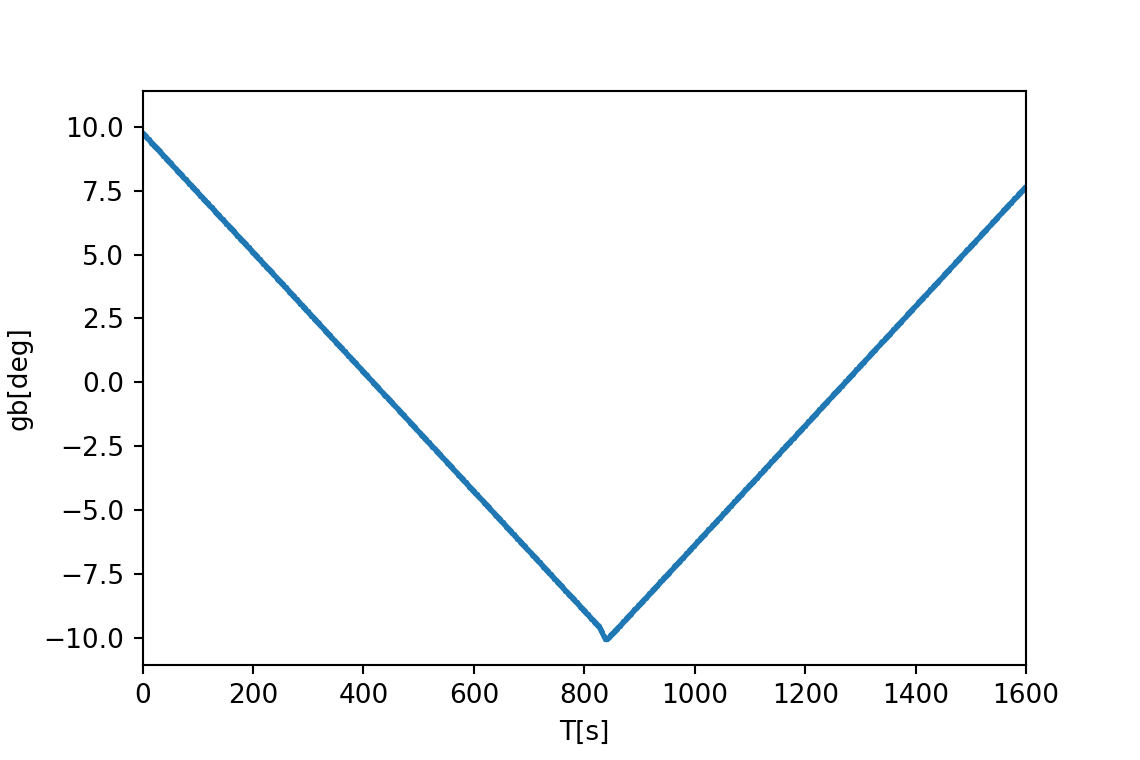
\includegraphics[width=0.58\textwidth]{figures/01634_0001-gb}
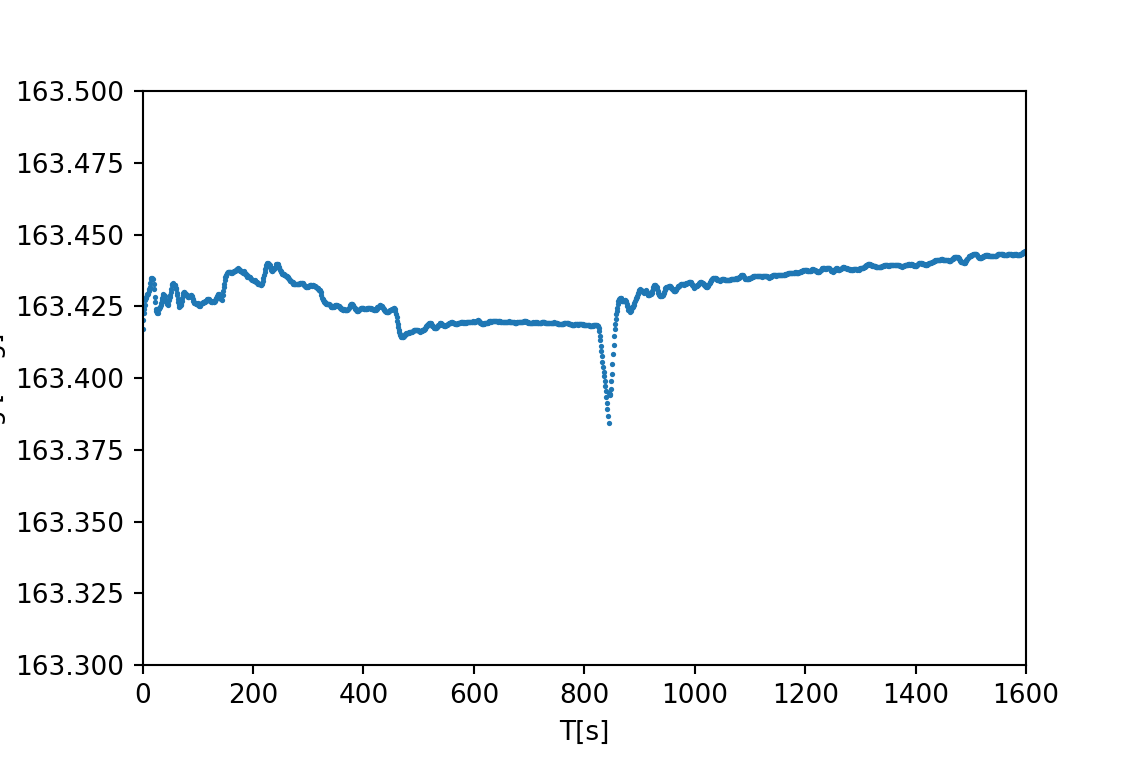
\includegraphics[width=0.58\textwidth]{figures/01634_0001-gl}
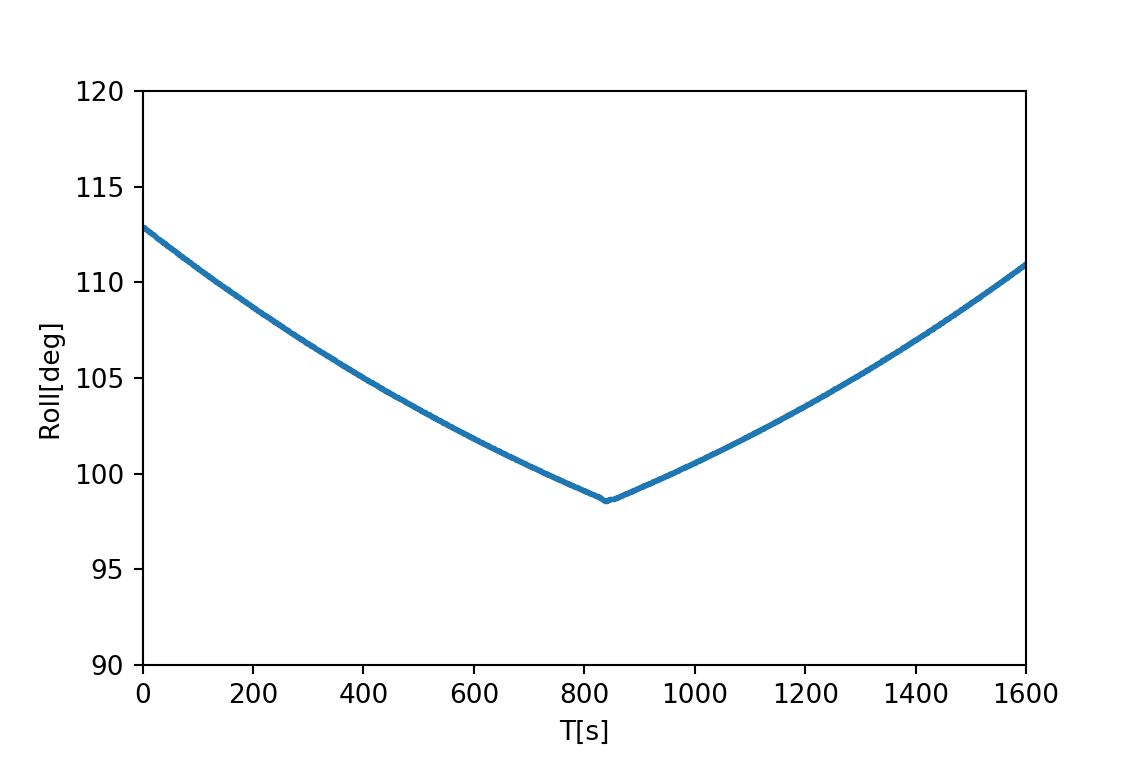
\includegraphics[width=0.58\textwidth]{figures/01634_0001-roll}
\end{center}
\caption{%
  \label{telescope}
  An example shows how the \galex\ telescope pointing and rotation change during one scan.
  The telescope traversed the Galactic plane twice during one scan and maitain the pointting in gl nearly unchanged.
  There are 450 scans similar to this have been observed during the \scanmode. 
  \emph{Top:}  Pointting in gb as a function of time;
  \emph{Middle:} Pointting in gl as a function of time;
  \emph{Bottom:} Rotation changes as a function of time.
}
\end{figure}

\begin{figure}[p]
\begin{center}
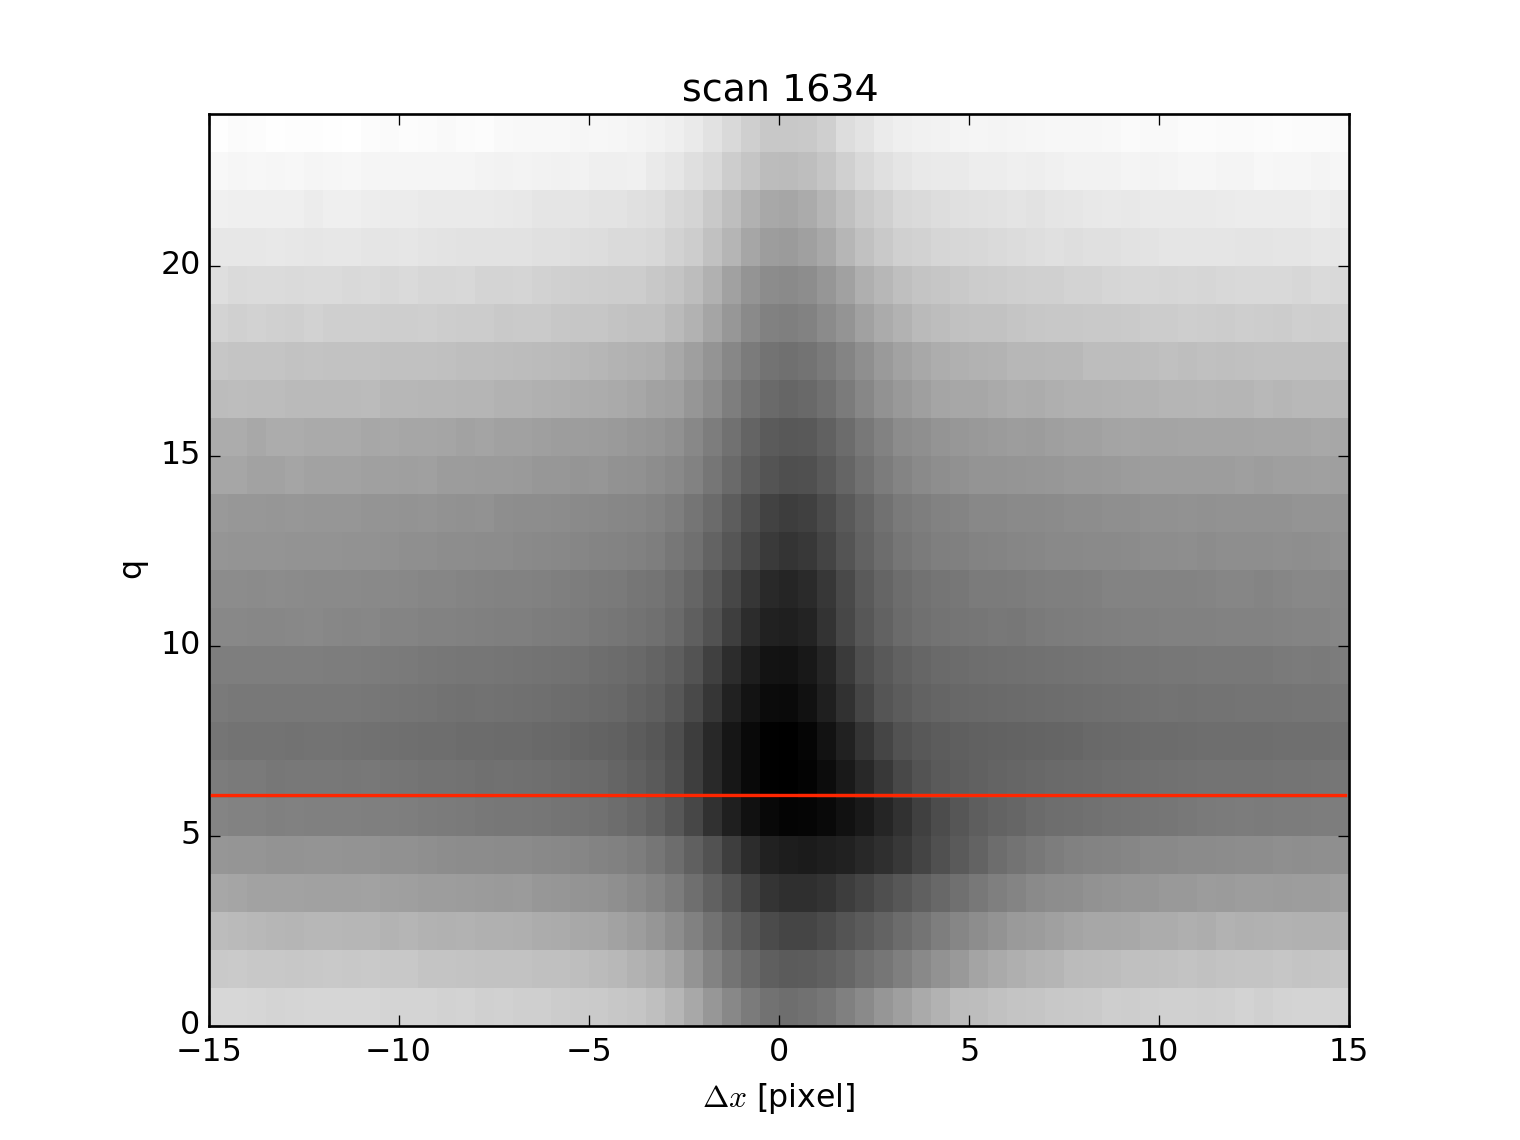
\includegraphics[width=0.49\textwidth]{figures/q-x_tot}
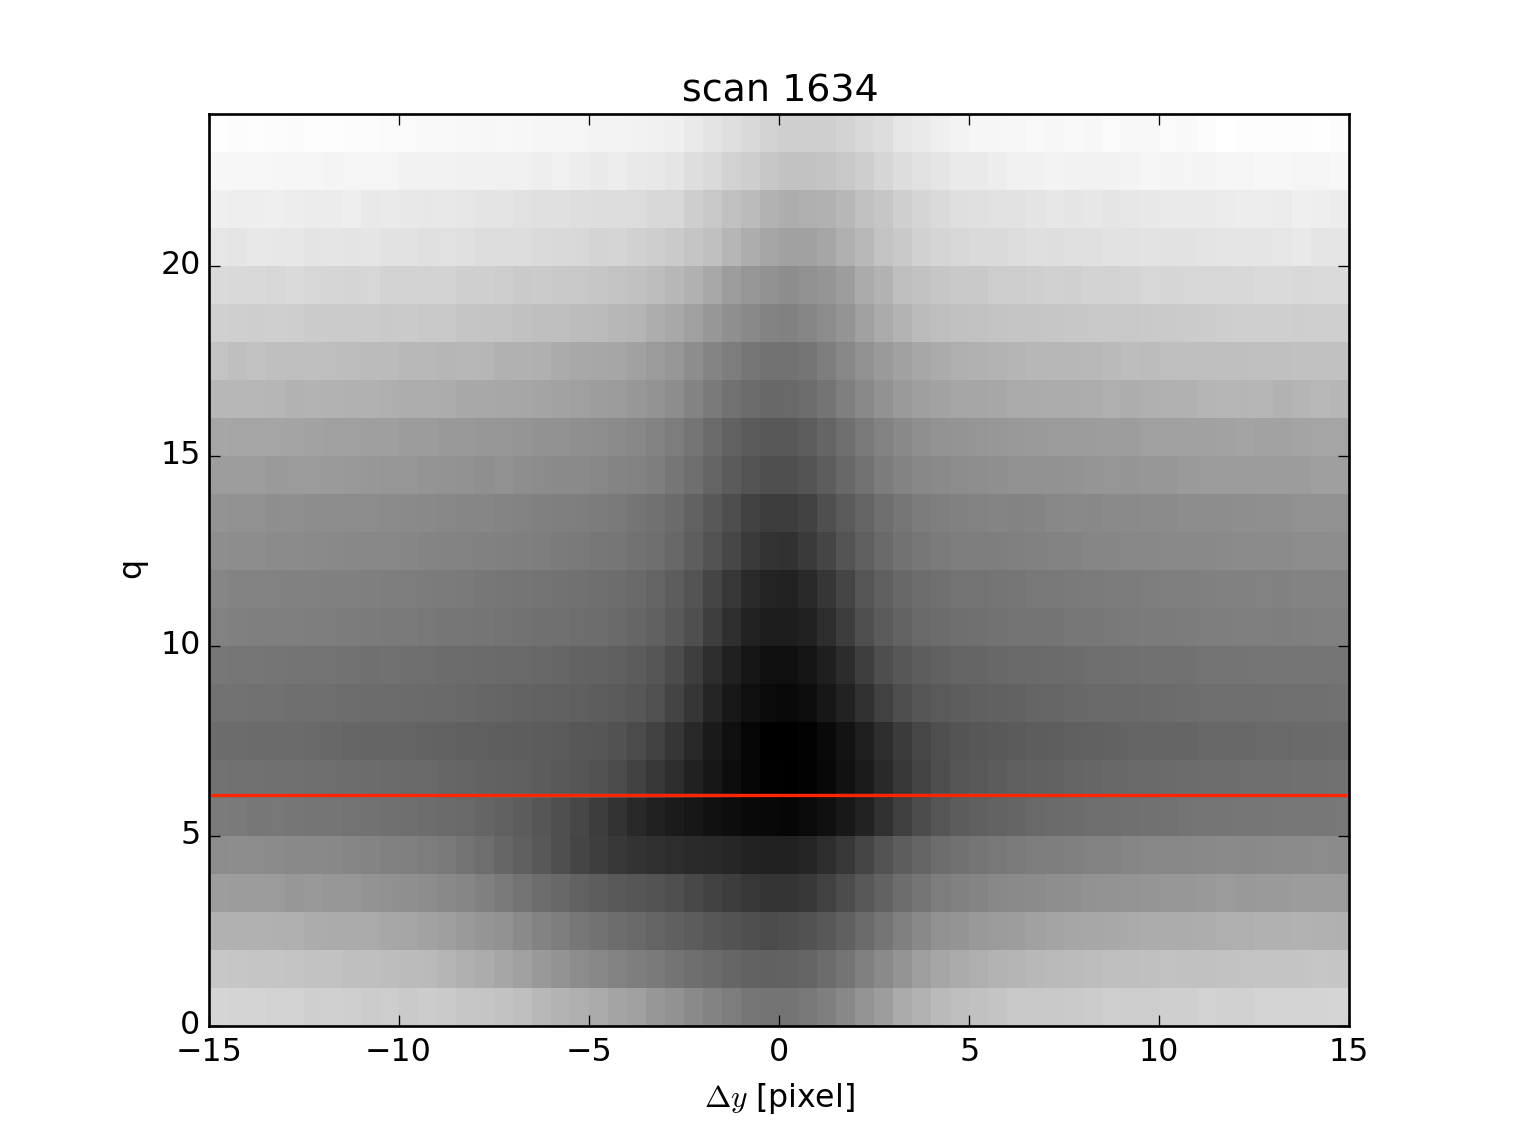
\includegraphics[width=0.49\textwidth]{figures/q-y_tot}
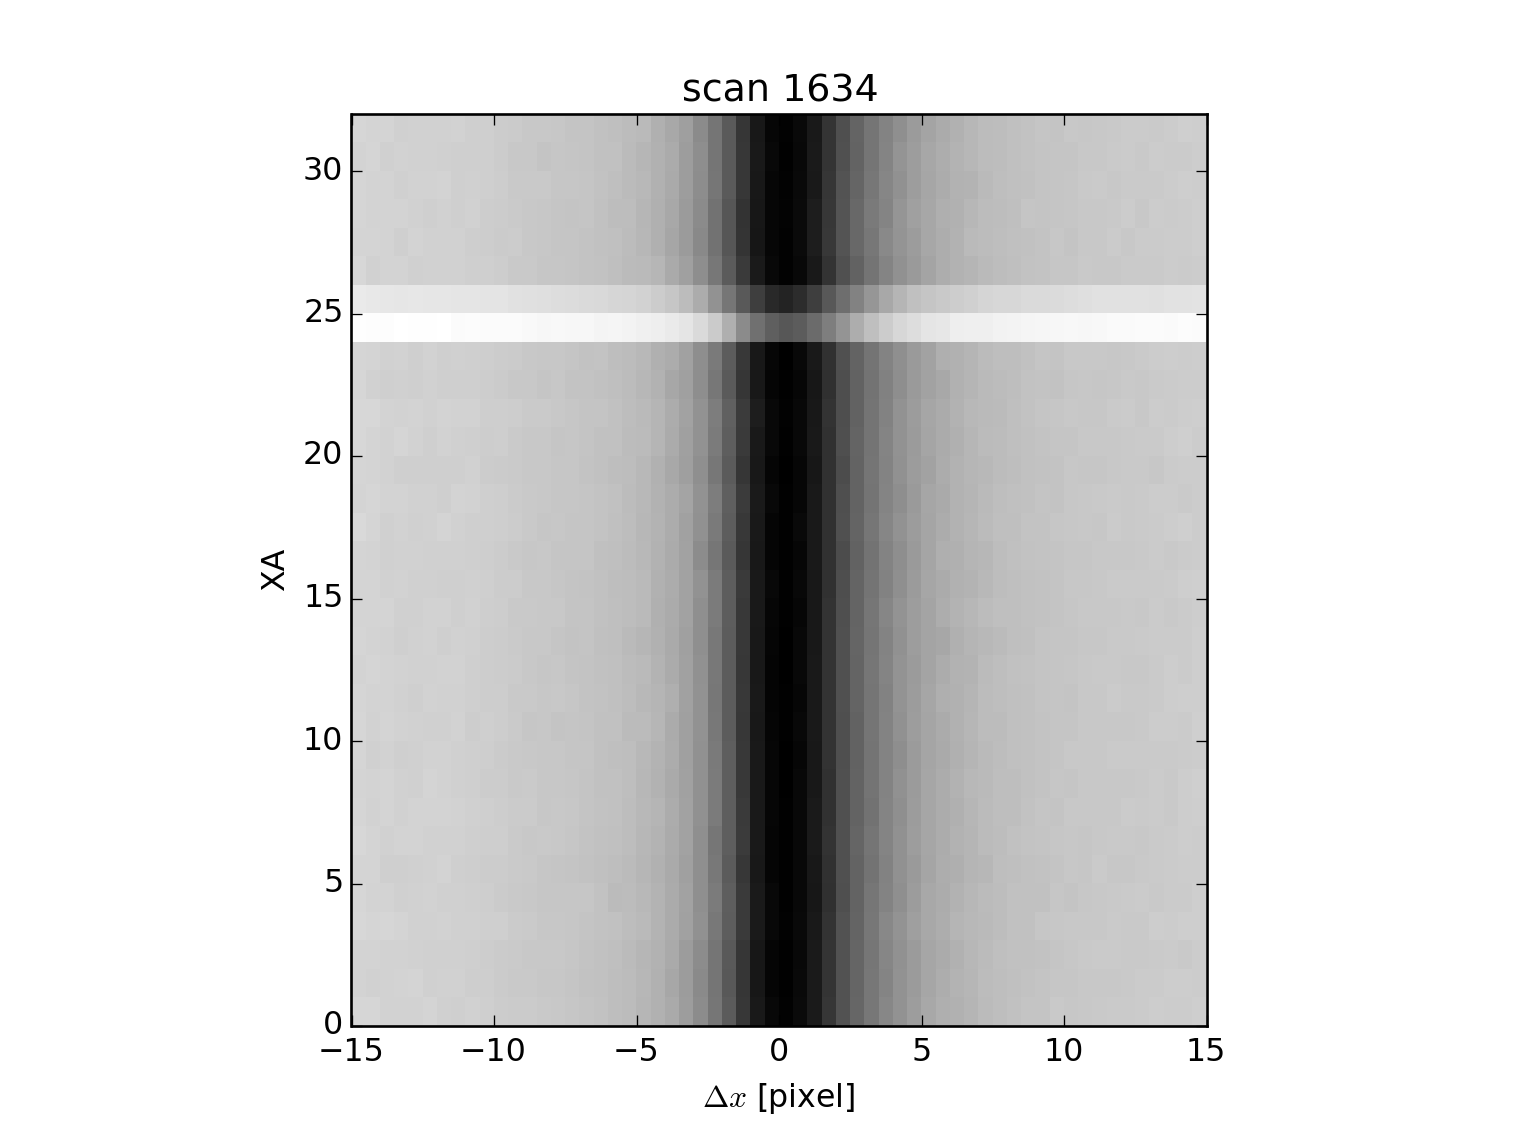
\includegraphics[width=0.49\textwidth]{figures/xa-x_tot}
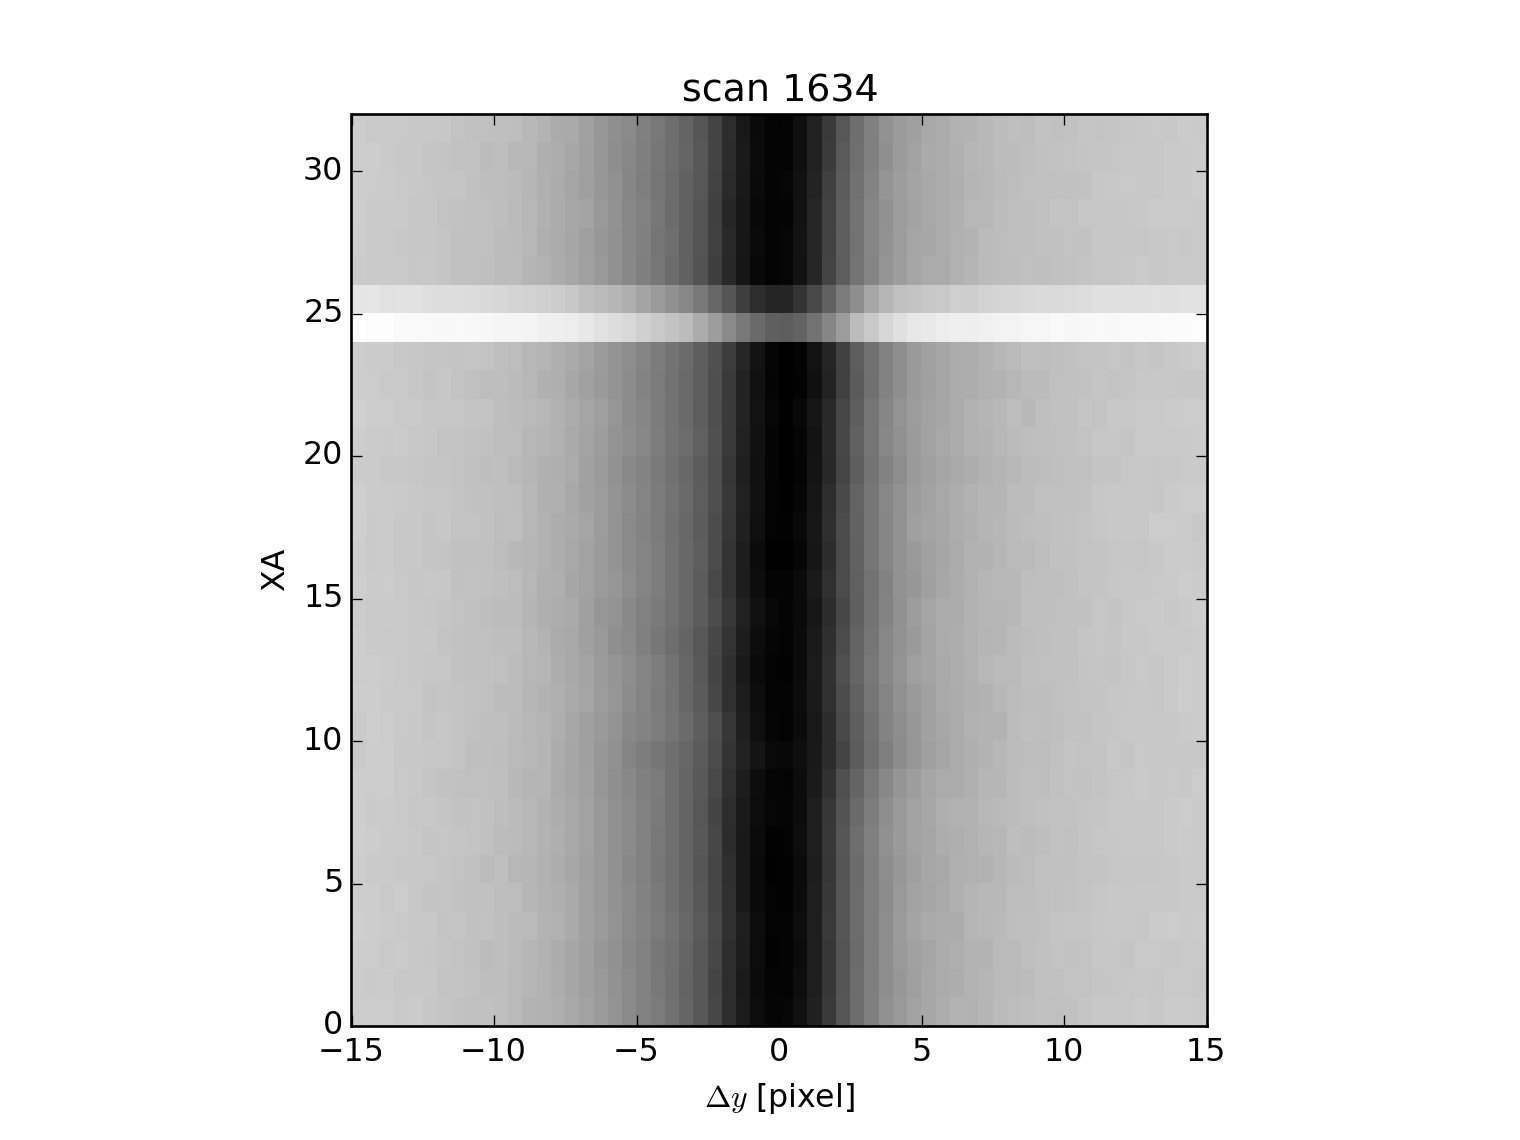
\includegraphics[width=0.49\textwidth]{figures/xa-y_tot}
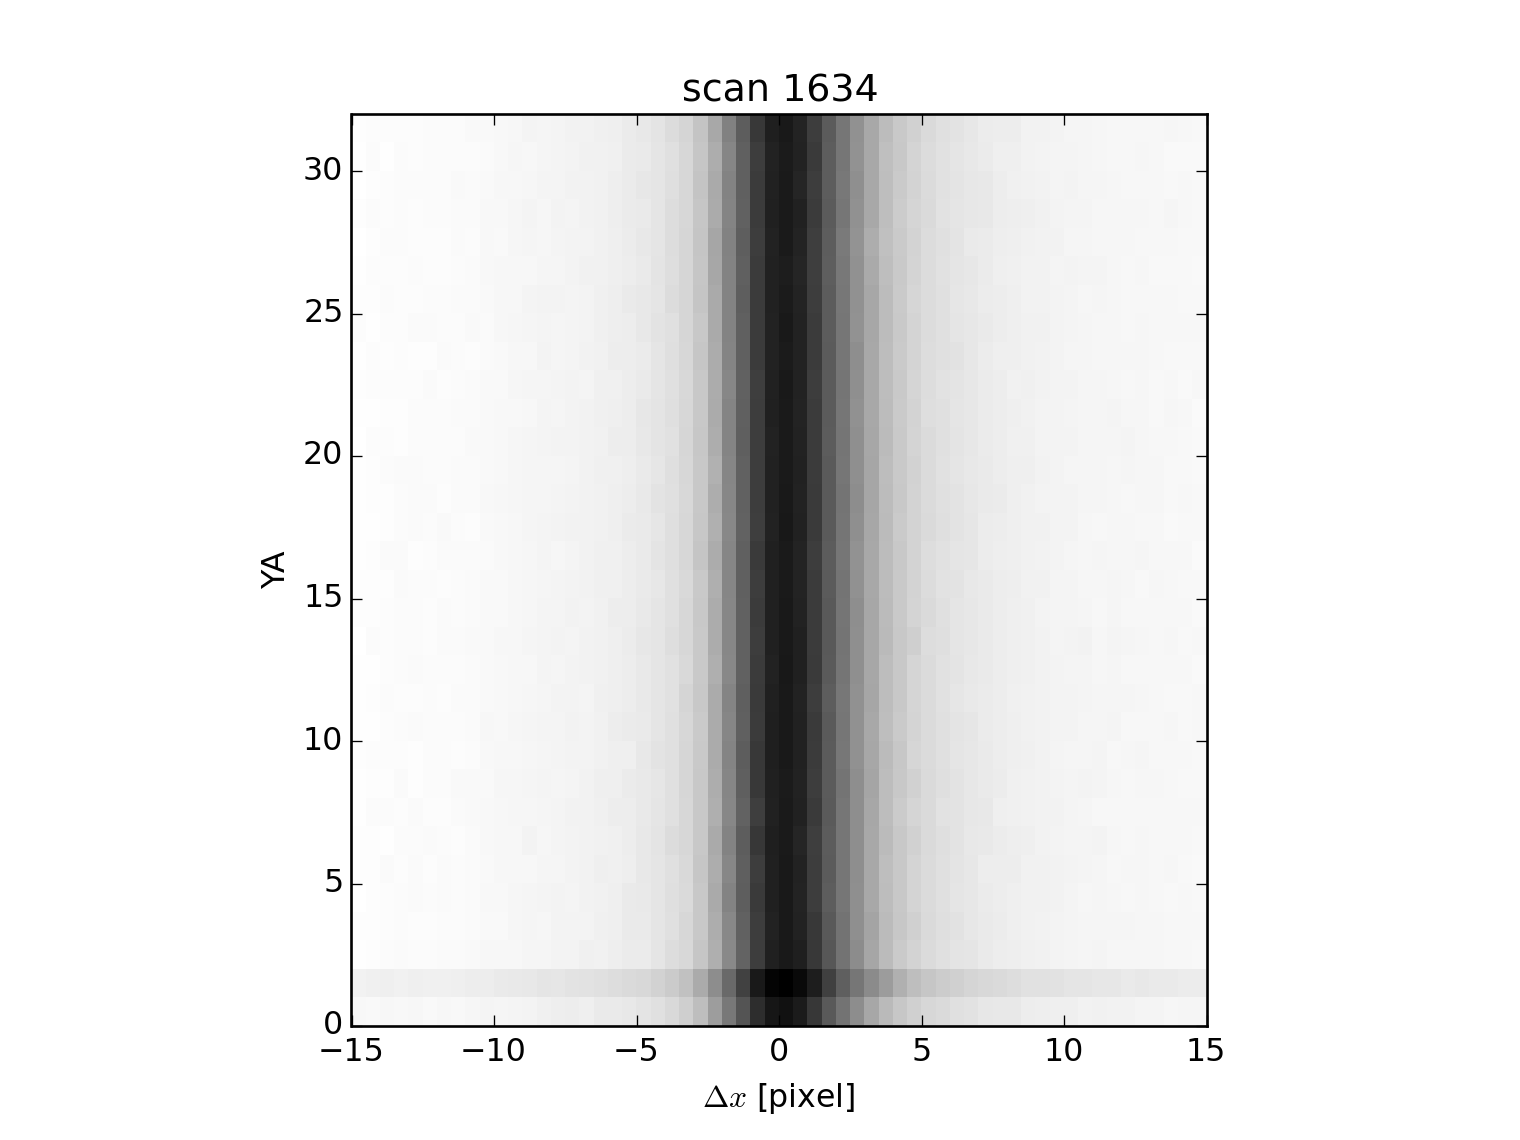
\includegraphics[width=0.49\textwidth]{figures/ya-x_tot}
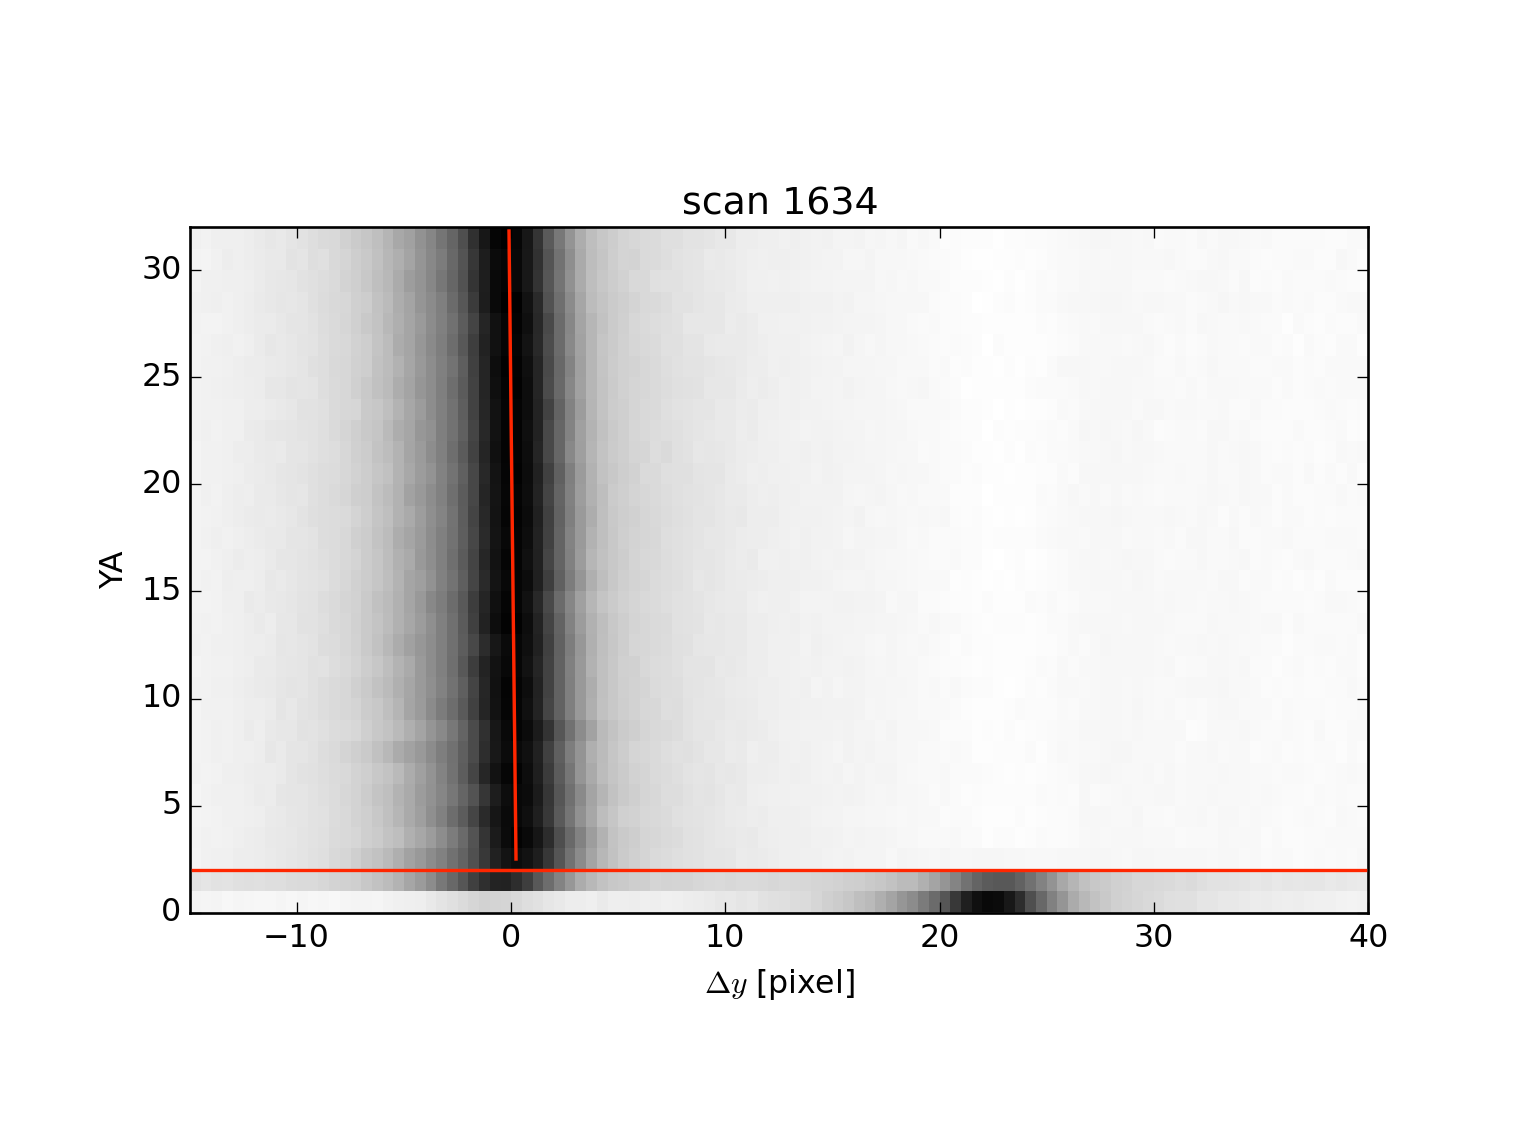
\includegraphics[width=0.49\textwidth]{figures/ya-y_tot}
\end{center}
\caption{%
  \label{meta}
  Overall offsets of photons as function of pulse height $Q$,  wiggle (the phase of the TAC)  $X_A$,  stim spread slope $Y_A$.
  Photons belew the horizontal red lines are removed from the photon list.
  }
\end{figure}

\section{Pointing calibration}
\label{pc}
As mentioned in Section \ref{data}, the \galex\ photons are tagged with time, position on the detector and other housekeeping information($Q$, $X_A$ and $Y_A$).
To use these photons such as constructing sky-maps, the pointing of the spacecraft is required as an input of the 
\project{gPhoton} to project the photons onto the sky.
Due to the nontrivial dithering pattern of \galex, the pointing recorded on the flight is not perfect, especially in the \scanmode, in which the spacecraft traversed the galactic plane rapidly. 
In this paper, we are going to use the photons together with the stars catalog to calibrate the pointing of the spacecraft.
The top plot in Fig.~\ref{slice} shows an one-second snapshot of the photons on the sky.
The stars from Tycho 2 catalog \citep{tycho2} in the same region are also plotted. 
It is obvious that there is an significant overall offset between the stars (cross-hair) and photons (points),  which is due to the imperfection of the pointing.
To characterize the offsets of the pointing of the spacecraft, the cross-correlation of photons and star catalog are calculated.
The cross-correlation $\xi(\vec{r})$ is defined as the count of photon-star pairs as a function of displacement $\vec{r}$.
As shown in the bottom plot of Fig.~\ref{slice}, the offsets of the pointing are determined by the centroid of the cross-correlation function. 
The shape of the correlation function is determined by the point spreading function (PSF).
There is also a secondary peak in the cross-correlation function due to the photons with $Y_A<2$, which has been explained in Section \ref{data} and can be removed by cutting the photon list.
After photons are binned in one-second slots, the offsets of pointing can be measured as a function of time as shown in Fig.~\ref{pointing}.

\begin{figure}[p]
\begin{center}
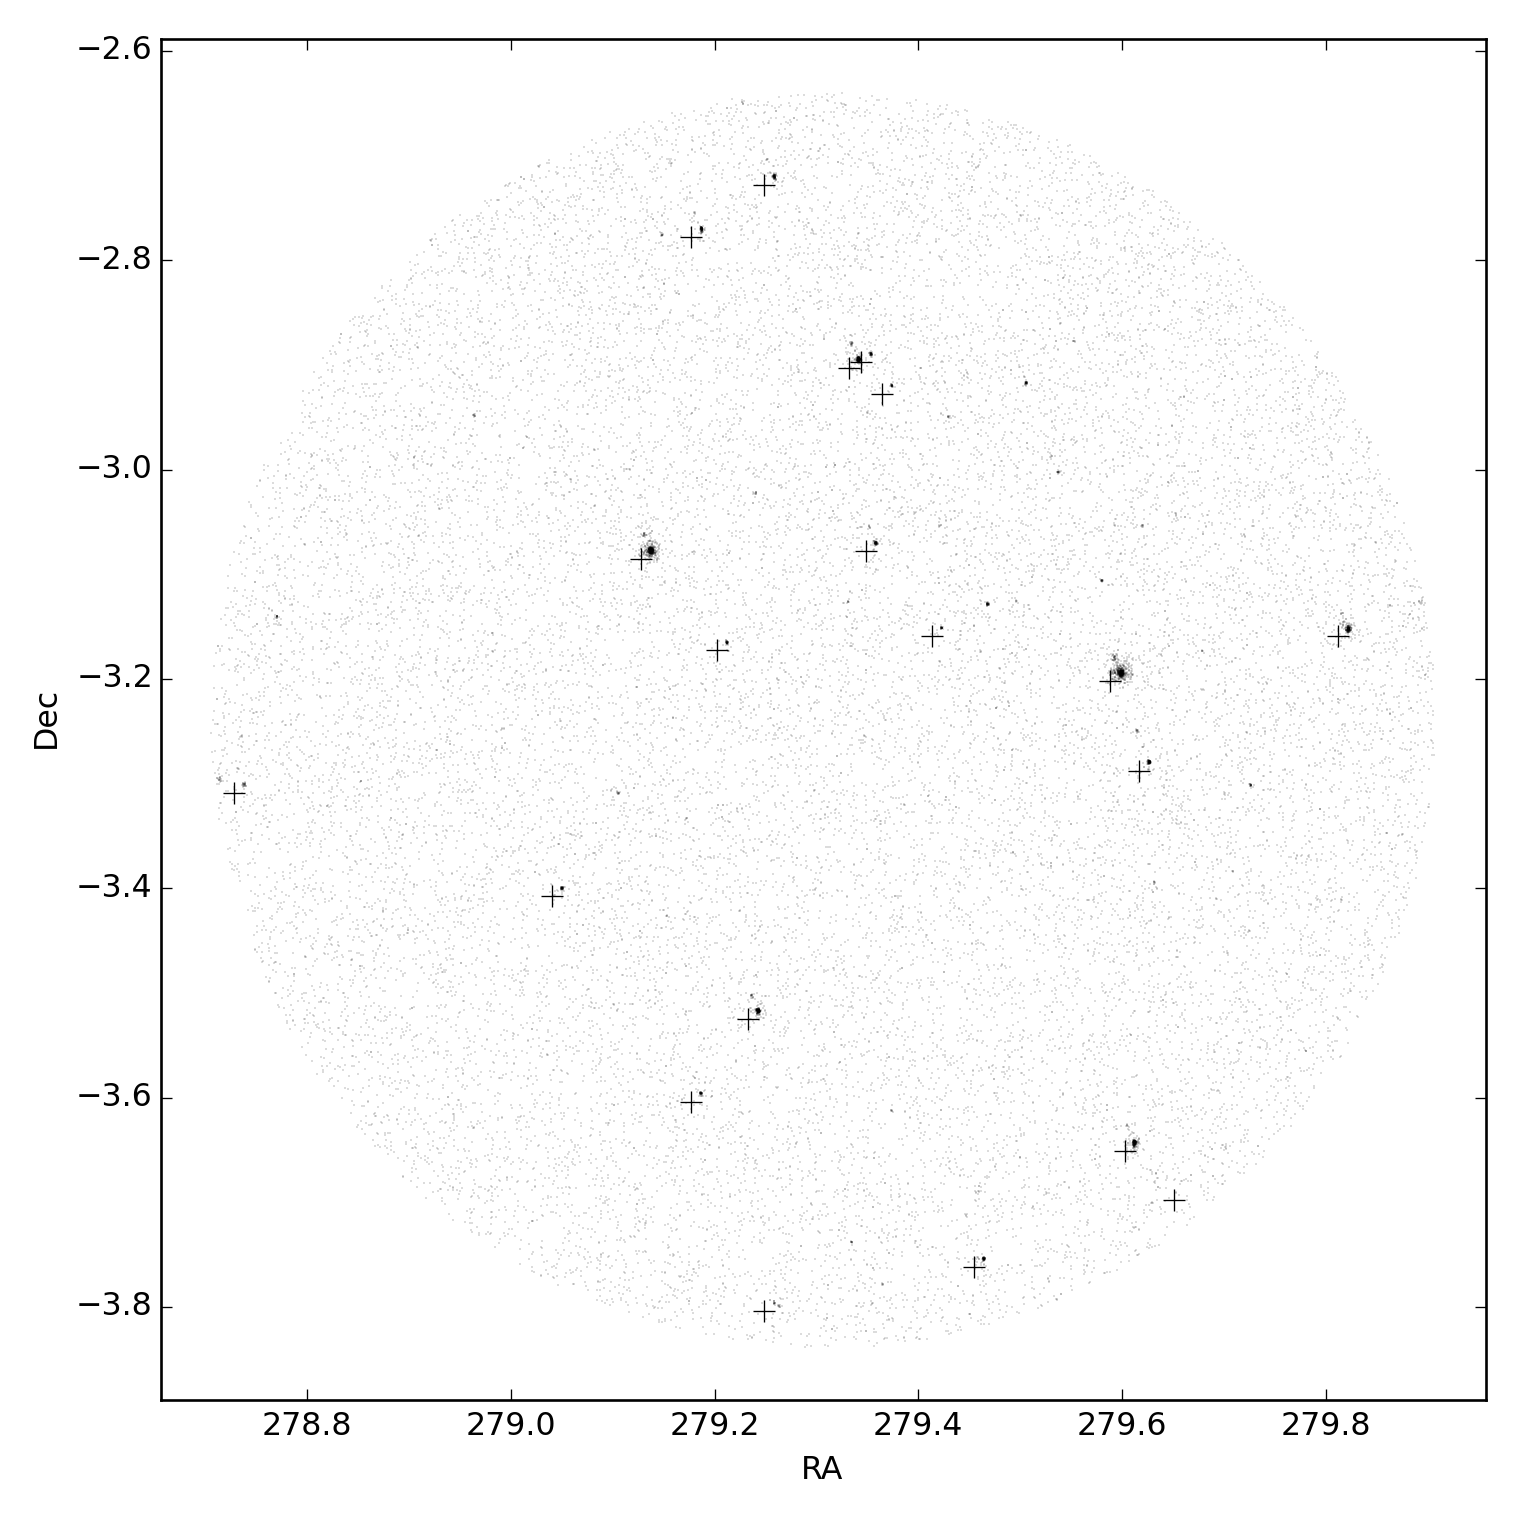
\includegraphics[width=0.535\textwidth]{figures/photons600}
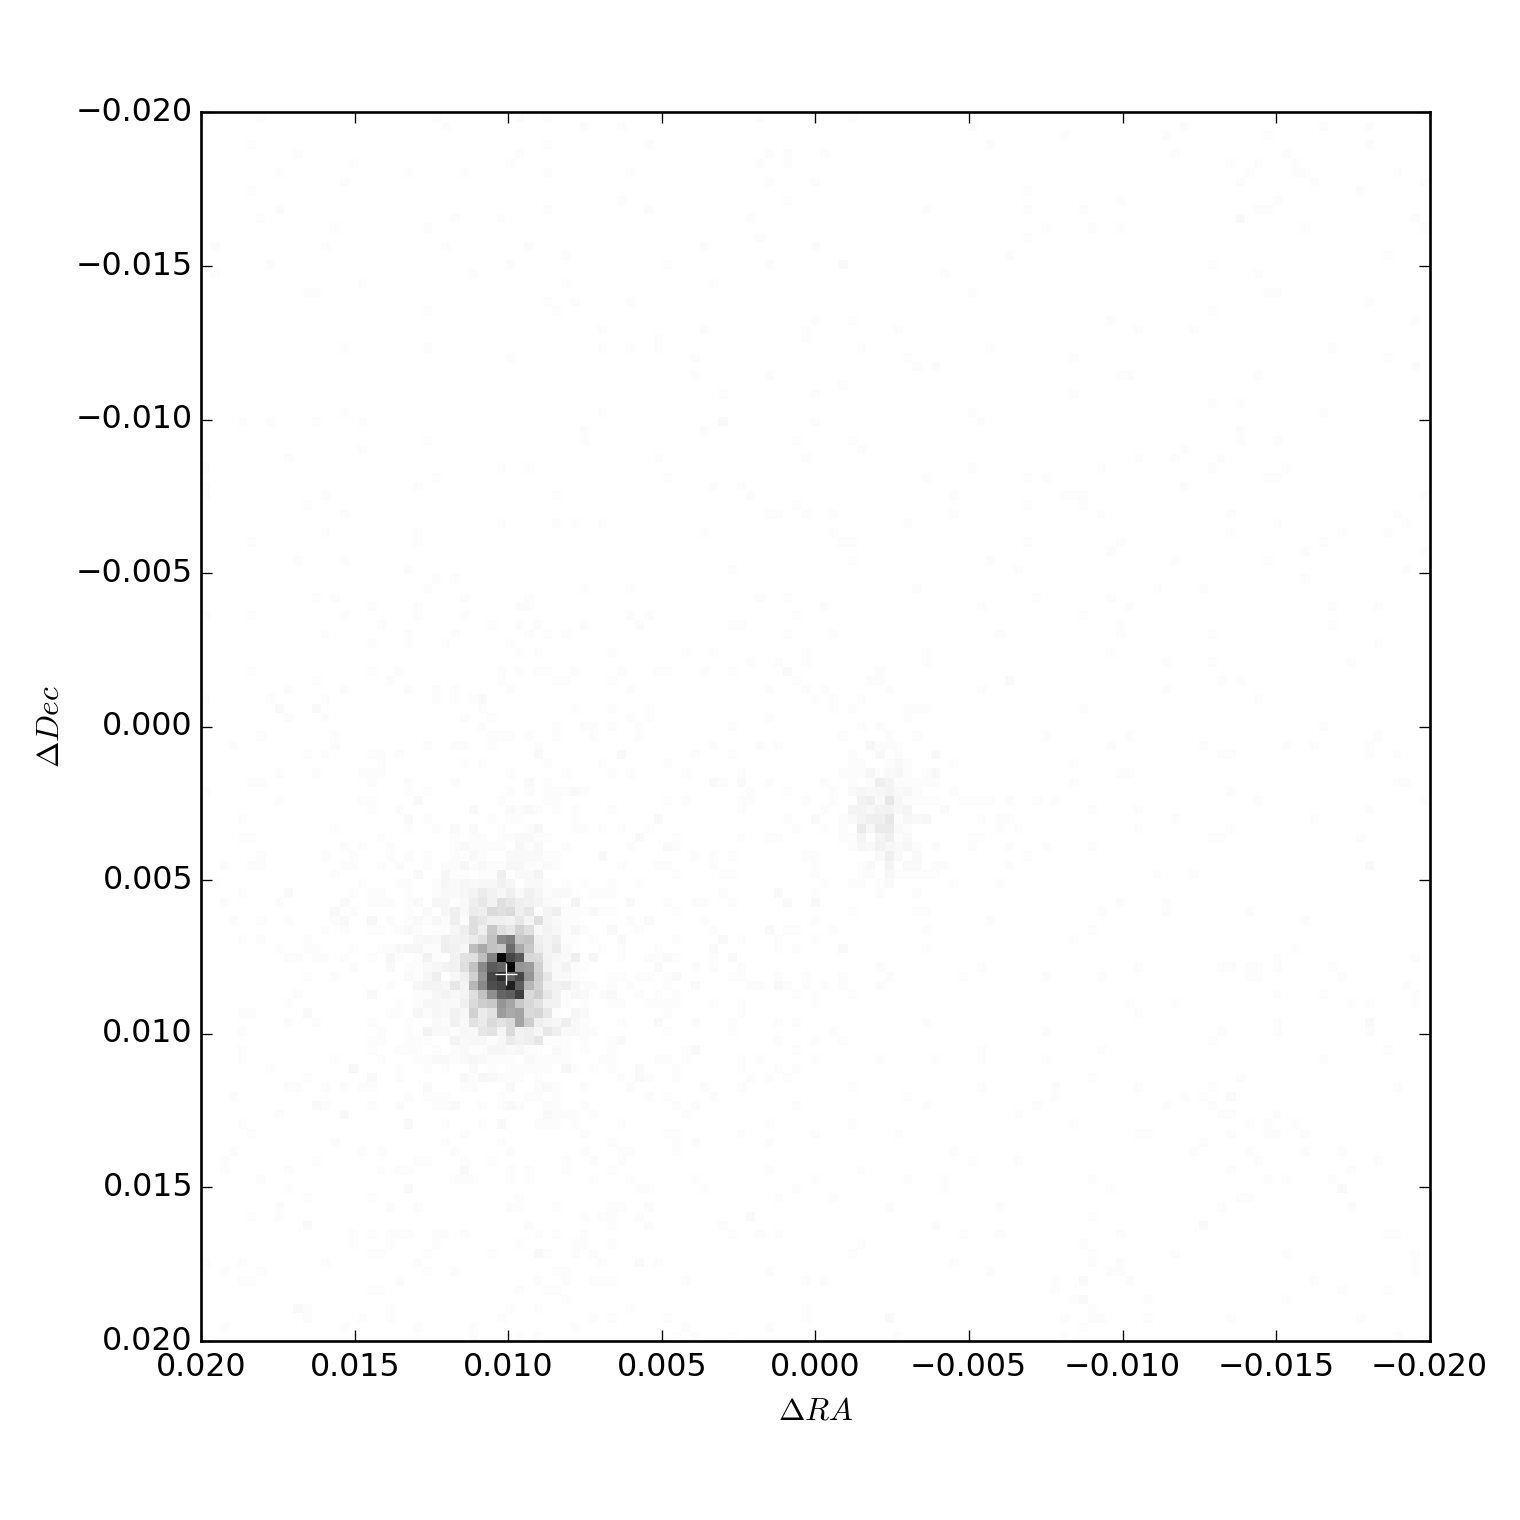
\includegraphics[width=0.58\textwidth]{figures/co600}
\end{center}
\caption{%
  \label{slice}
  Cross-correlation of photons and star catalog.
  \emph{Top:}  An one-second snapshot of the photons on the sky. The points are the location of the photons. The crosses indicate the location of the stars from the input catalog. It is obvious that there is a small offset between photons and the stars.
  \emph{Bottom:} The cross-correlation of photons and stars. 
  Each black points in the plot shows the offset between a pair of photon and star. 
  The white cross indicates the centroid of the cross-correlation fucntion, which is the overall offsets between photons and stars---the offset of the pointing.
  }
\end{figure}

\begin{figure}[p]
\begin{center}
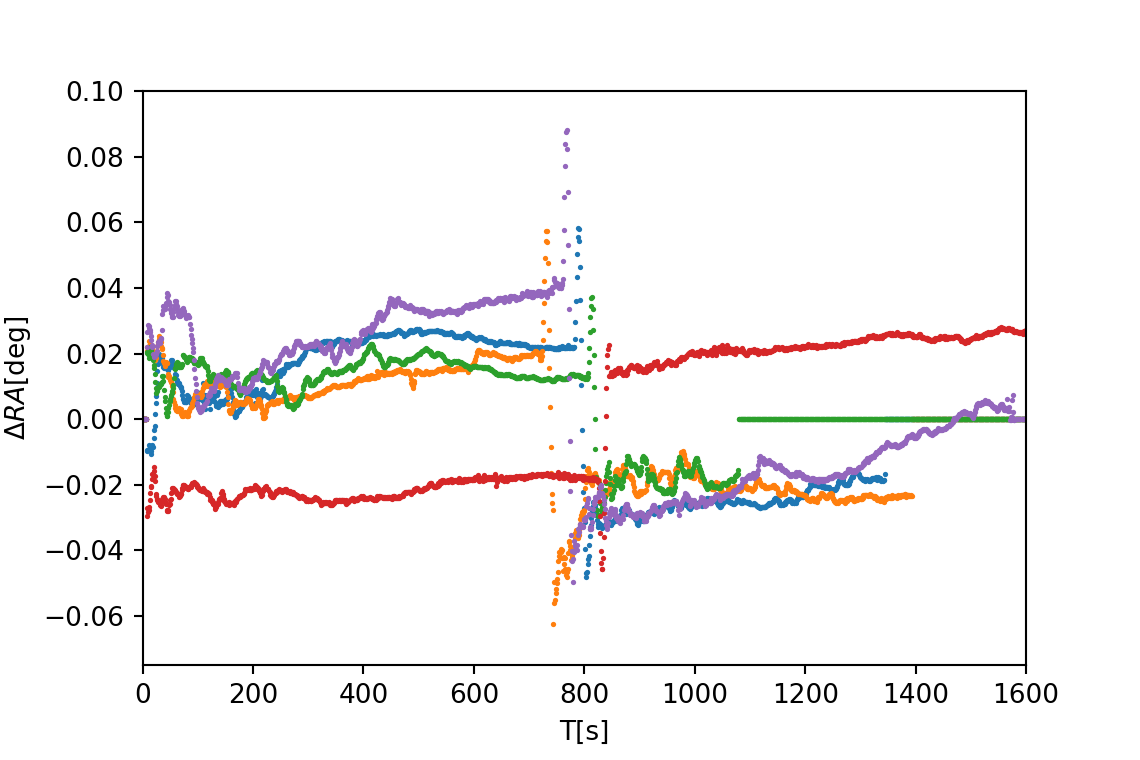
\includegraphics[width=0.6\textwidth]{figures/all-ra}
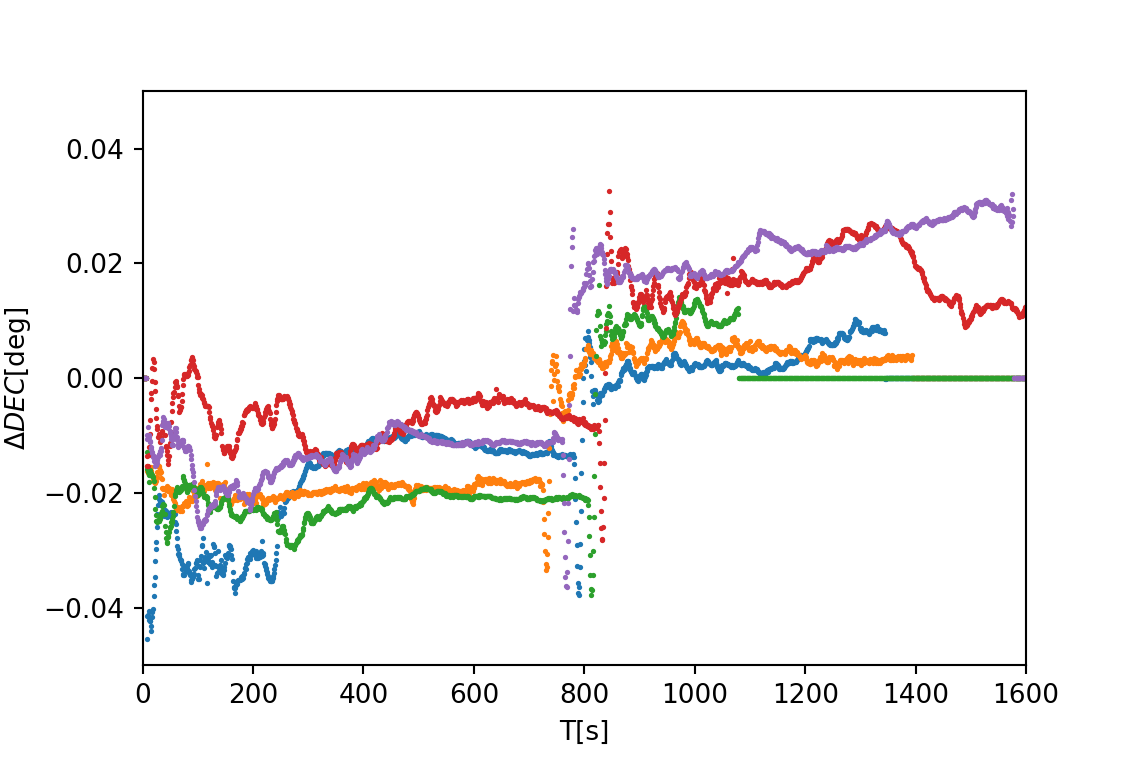
\includegraphics[width=0.6\textwidth]{figures/all-dec}
\end{center}
\caption{%
  \label{pointing}
  Pointing offsets as a function of time.
  \emph{Top:}  Pointing offsets in RA as a function of time.
  \emph{Bottom:} Pointing offsets in Dec as a function of time.
  The dramtical changes around 800s is due to the spacecraft turning over in the middle of the scan. 
  }
\end{figure}

\section{Distortion map}
\label{dm}
Except for the overall offset due to the pointing, there is also local error in photon position caused by the detector. 
According to \cite{galex_cal}, the photon position on \galex\ detector was measured by the arrival time difference of pulses from either side of the delay line anode, while the time difference consists of an integer number of coarse clock step and a fine position (phase of the coarse clock).
The fine position is measured as voltage value by time-to-amplitude converter (TAC).
Due to the electronic nonlinearity of TAC, each photon event can have a small local error in position and this effect is recorded as $X_A$ value in the photon list.
In addition to the nonlinearity of TAC, the variations in gain also affect the position of the photon events.
The gain effect is recorded as pulse height $Q$ in the photon list.
To calibrate these local effects on the detector, in this paper, a distortion map is constructed by a similar method in Section \ref{pc}.  
The detector is divided into 50 by 50 pixels. 
Within each pixel, the stars are projected onto the detector with the pointing measured in section \ref{pc}.
Then the photons and stars are cross-correlated and the centroid of the correlation function is measured as the distortion in that pixel location.
In Fig.~\ref{distortion_xa}, the photons are binned into three subset by the $X_A$ value and the distortion-map of each subset photons is constructed.
The amplitude of the distortion is about 0.03 pixels, which is approximately few arcsec on the sky.
There is significant difference between distortion-map constructed with different subset of photons.
The difference shows a periodic pattern over the detector, which is expected to account for the phases of the coarse clock.   
Similarly Fig.~\ref{distortion_q} shows the distortion-map constructed with photons of different $Q$ values.

\begin{figure}[p]
\begin{center}
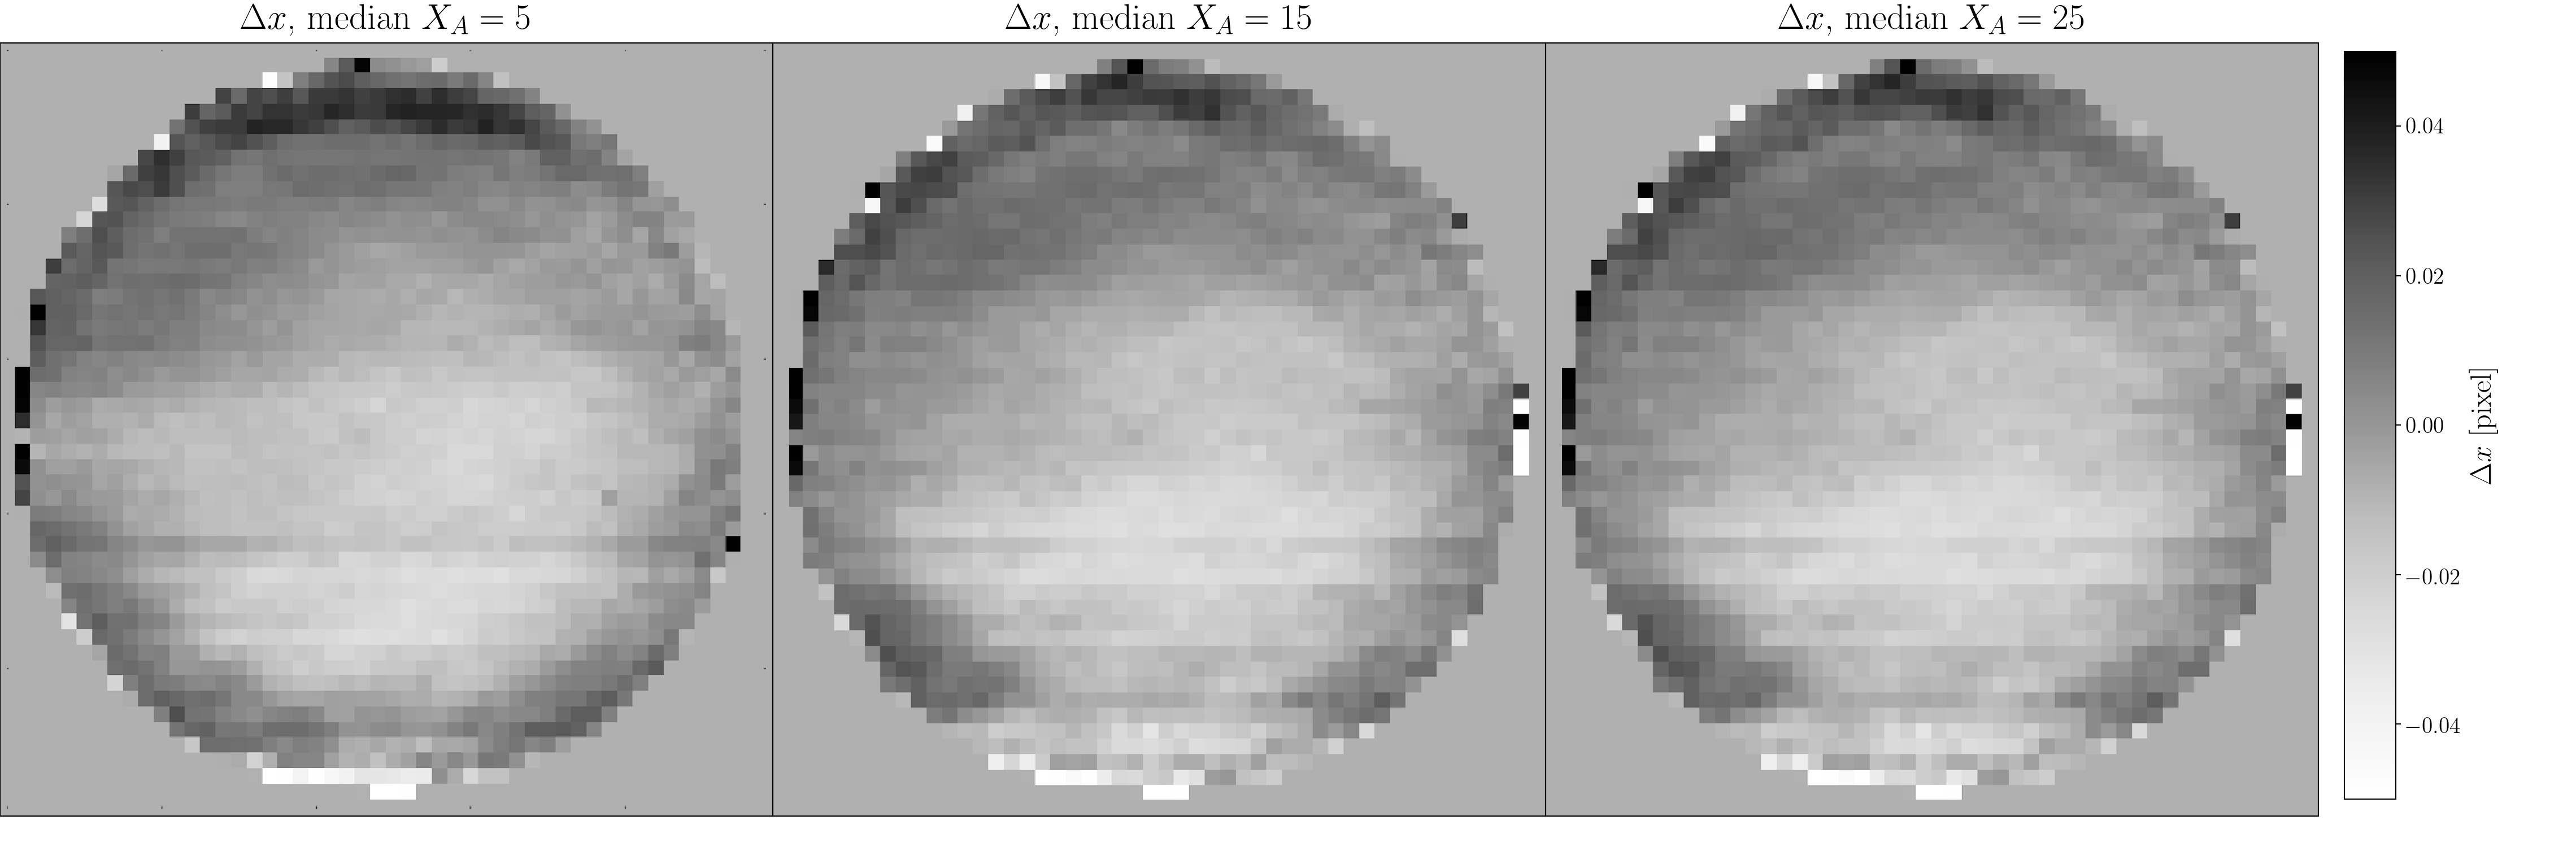
\includegraphics[width=0.95\textwidth]{figures/xa-x}
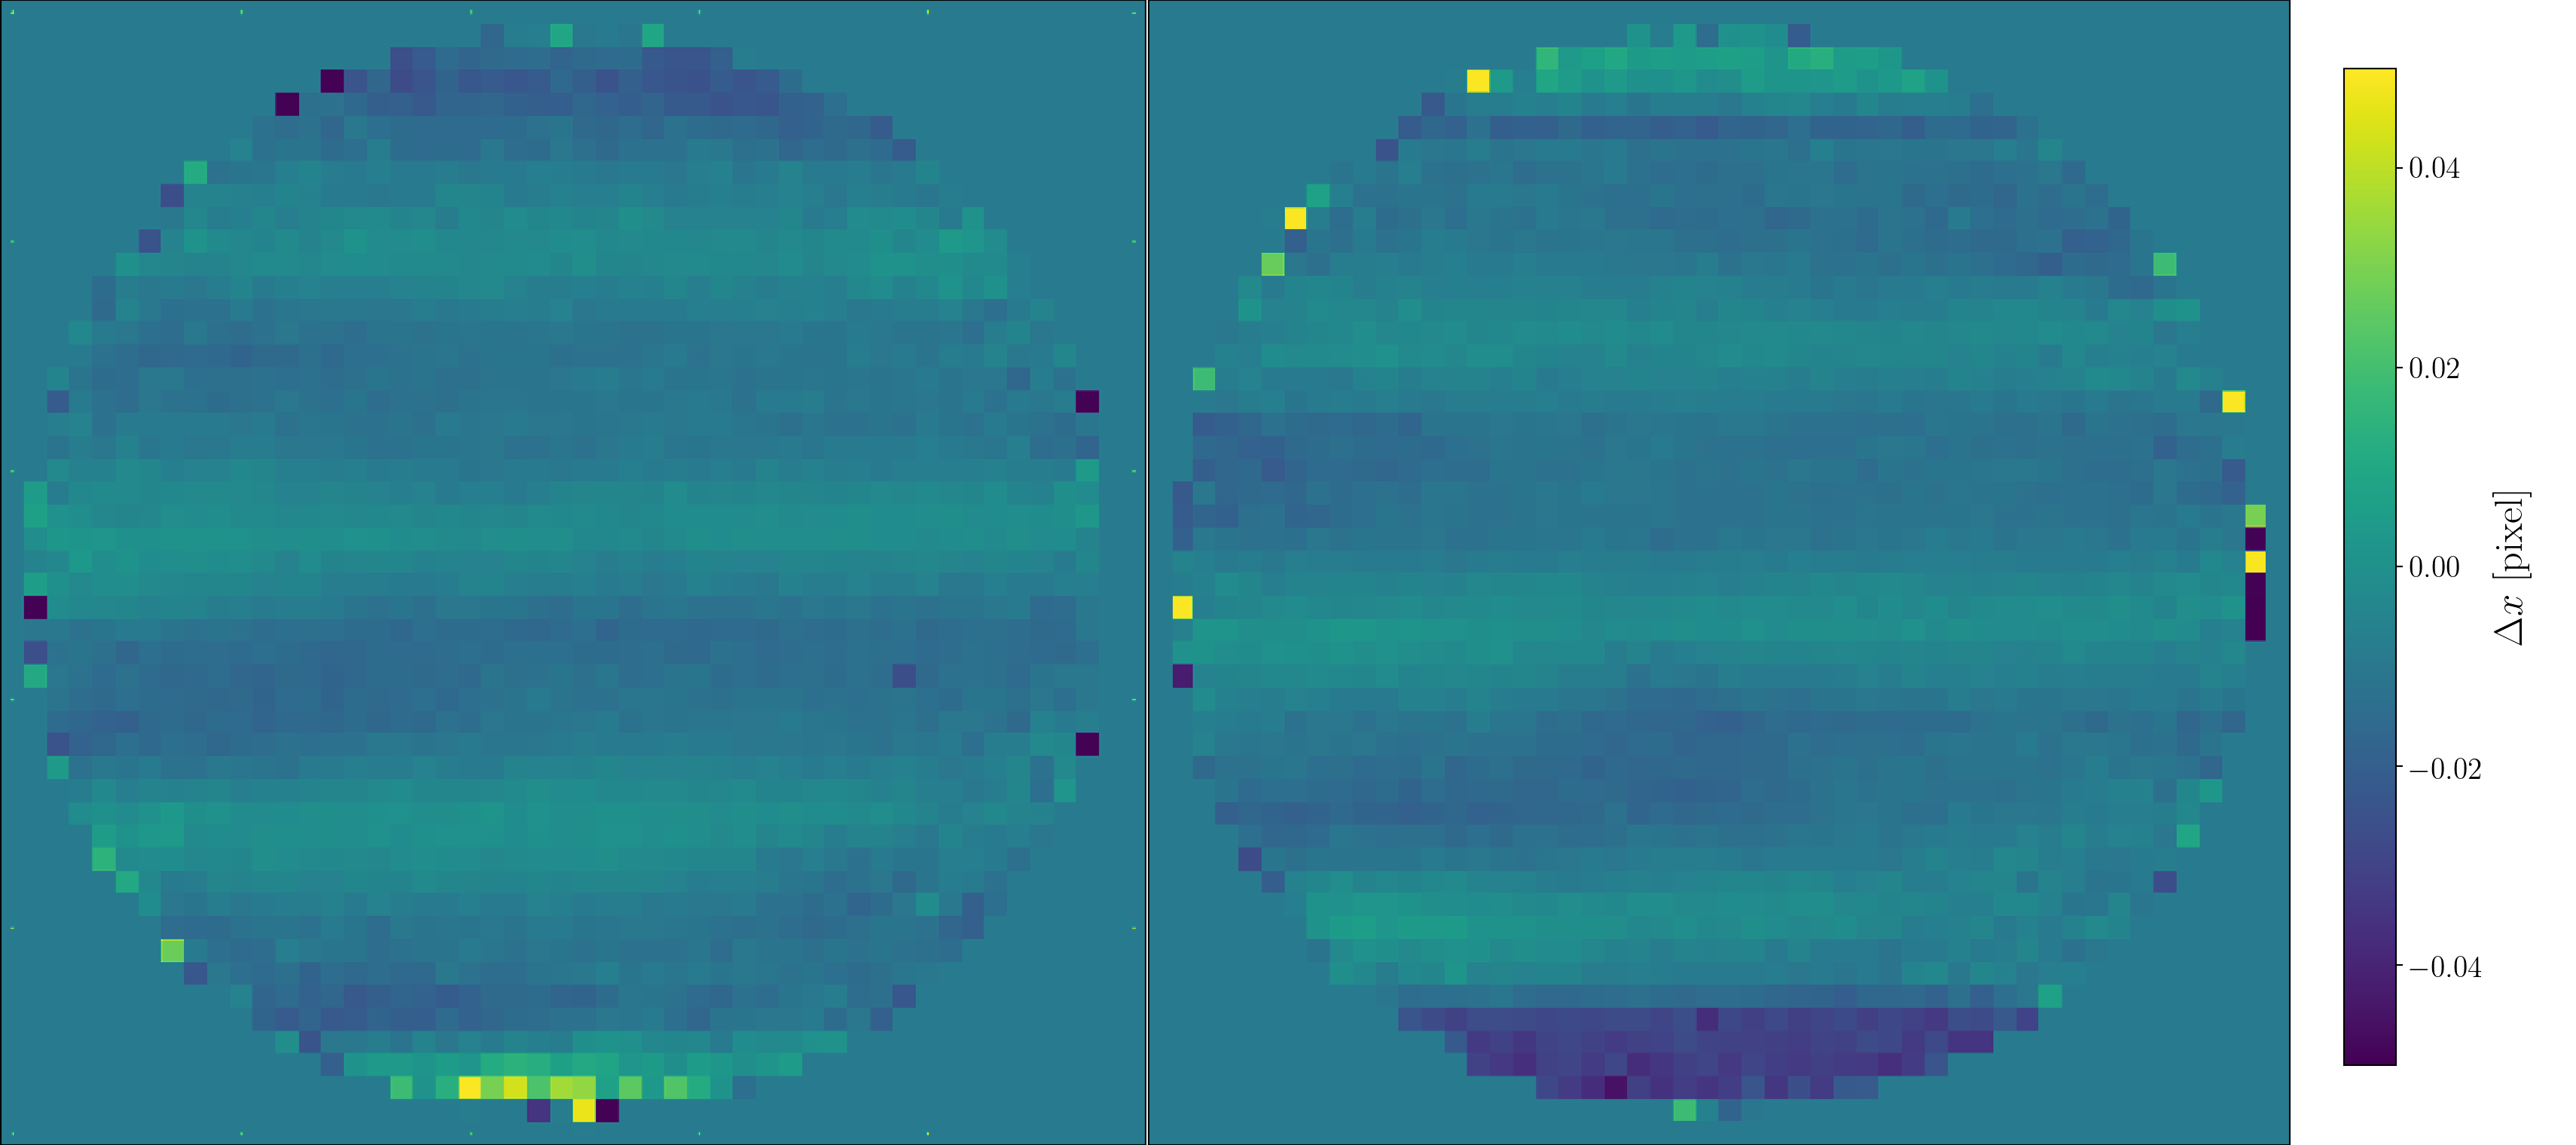
\includegraphics[width=0.6\textwidth]{figures/dif-xa-x}
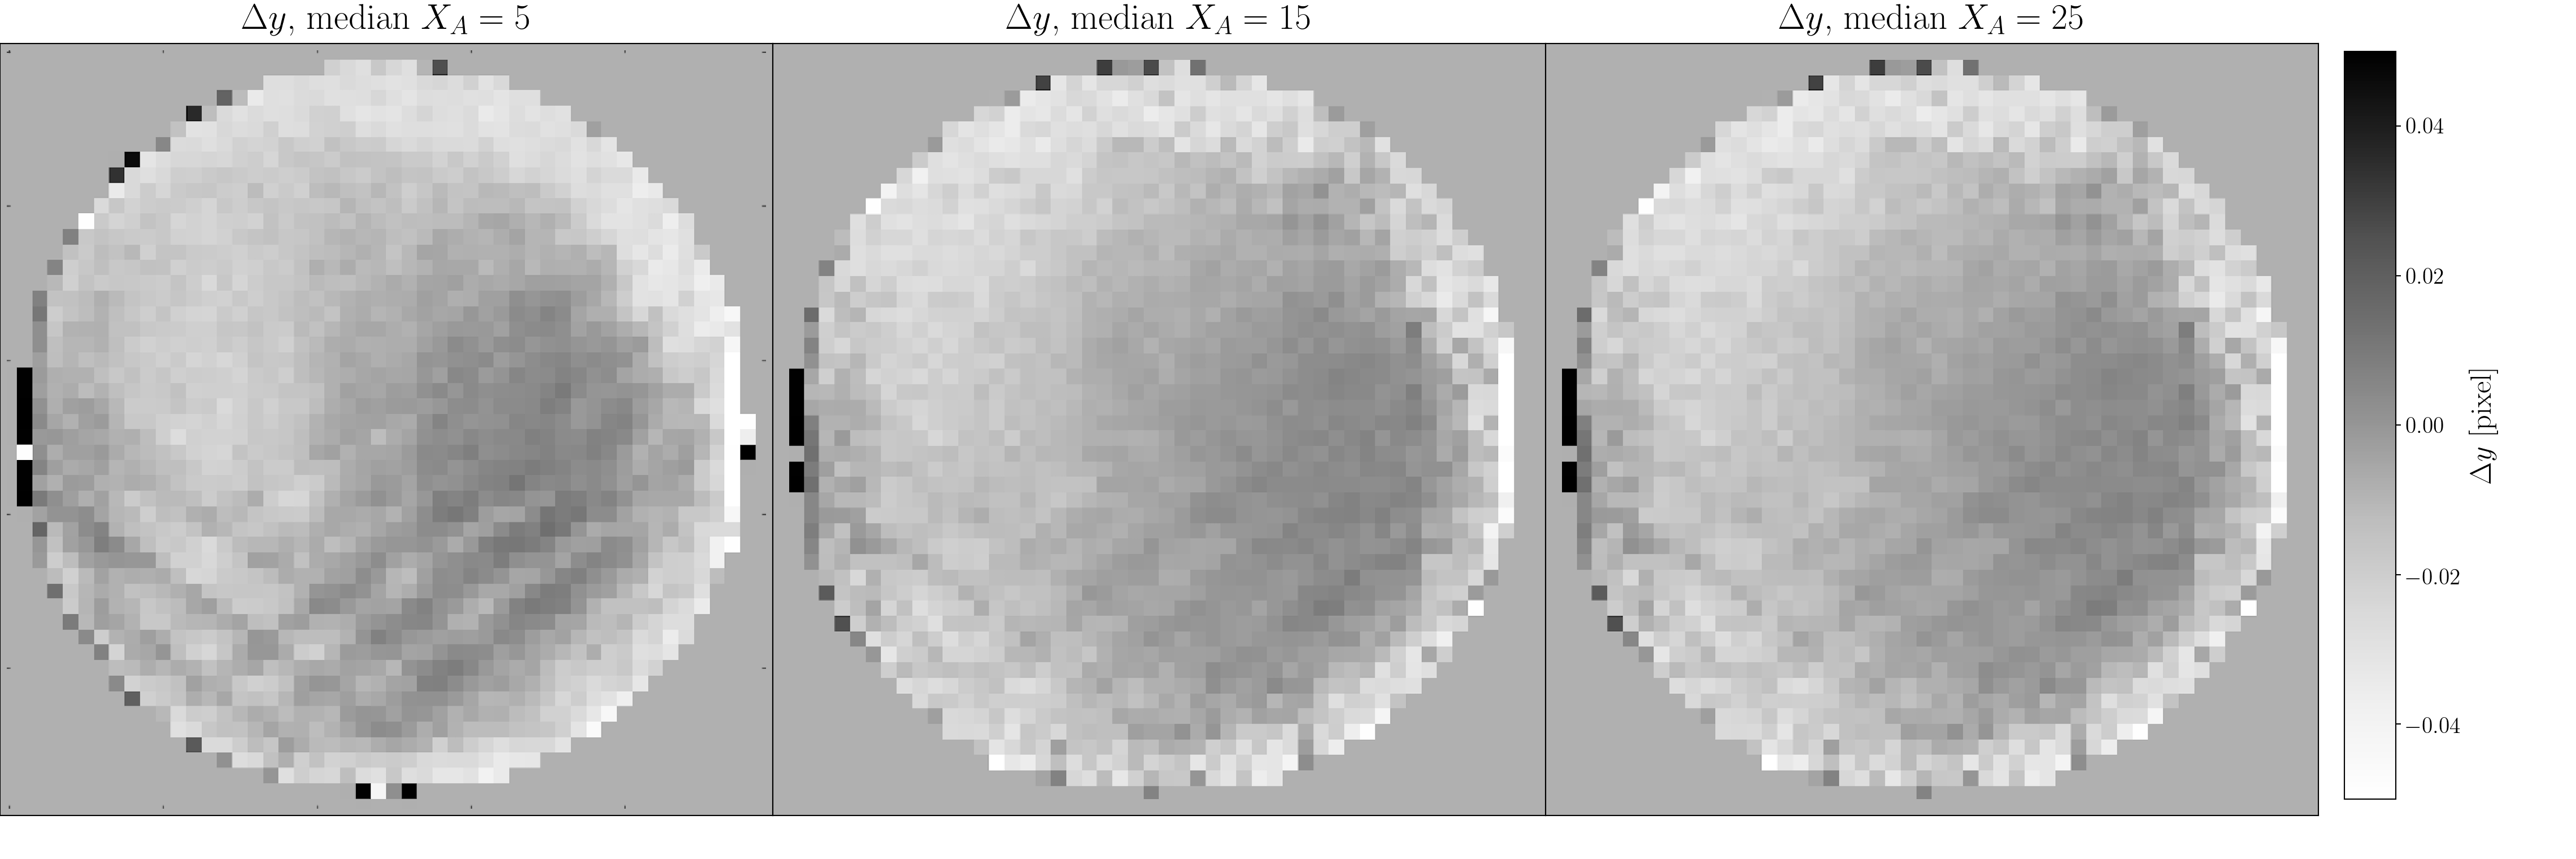
\includegraphics[width=0.95\textwidth]{figures/xa-y}
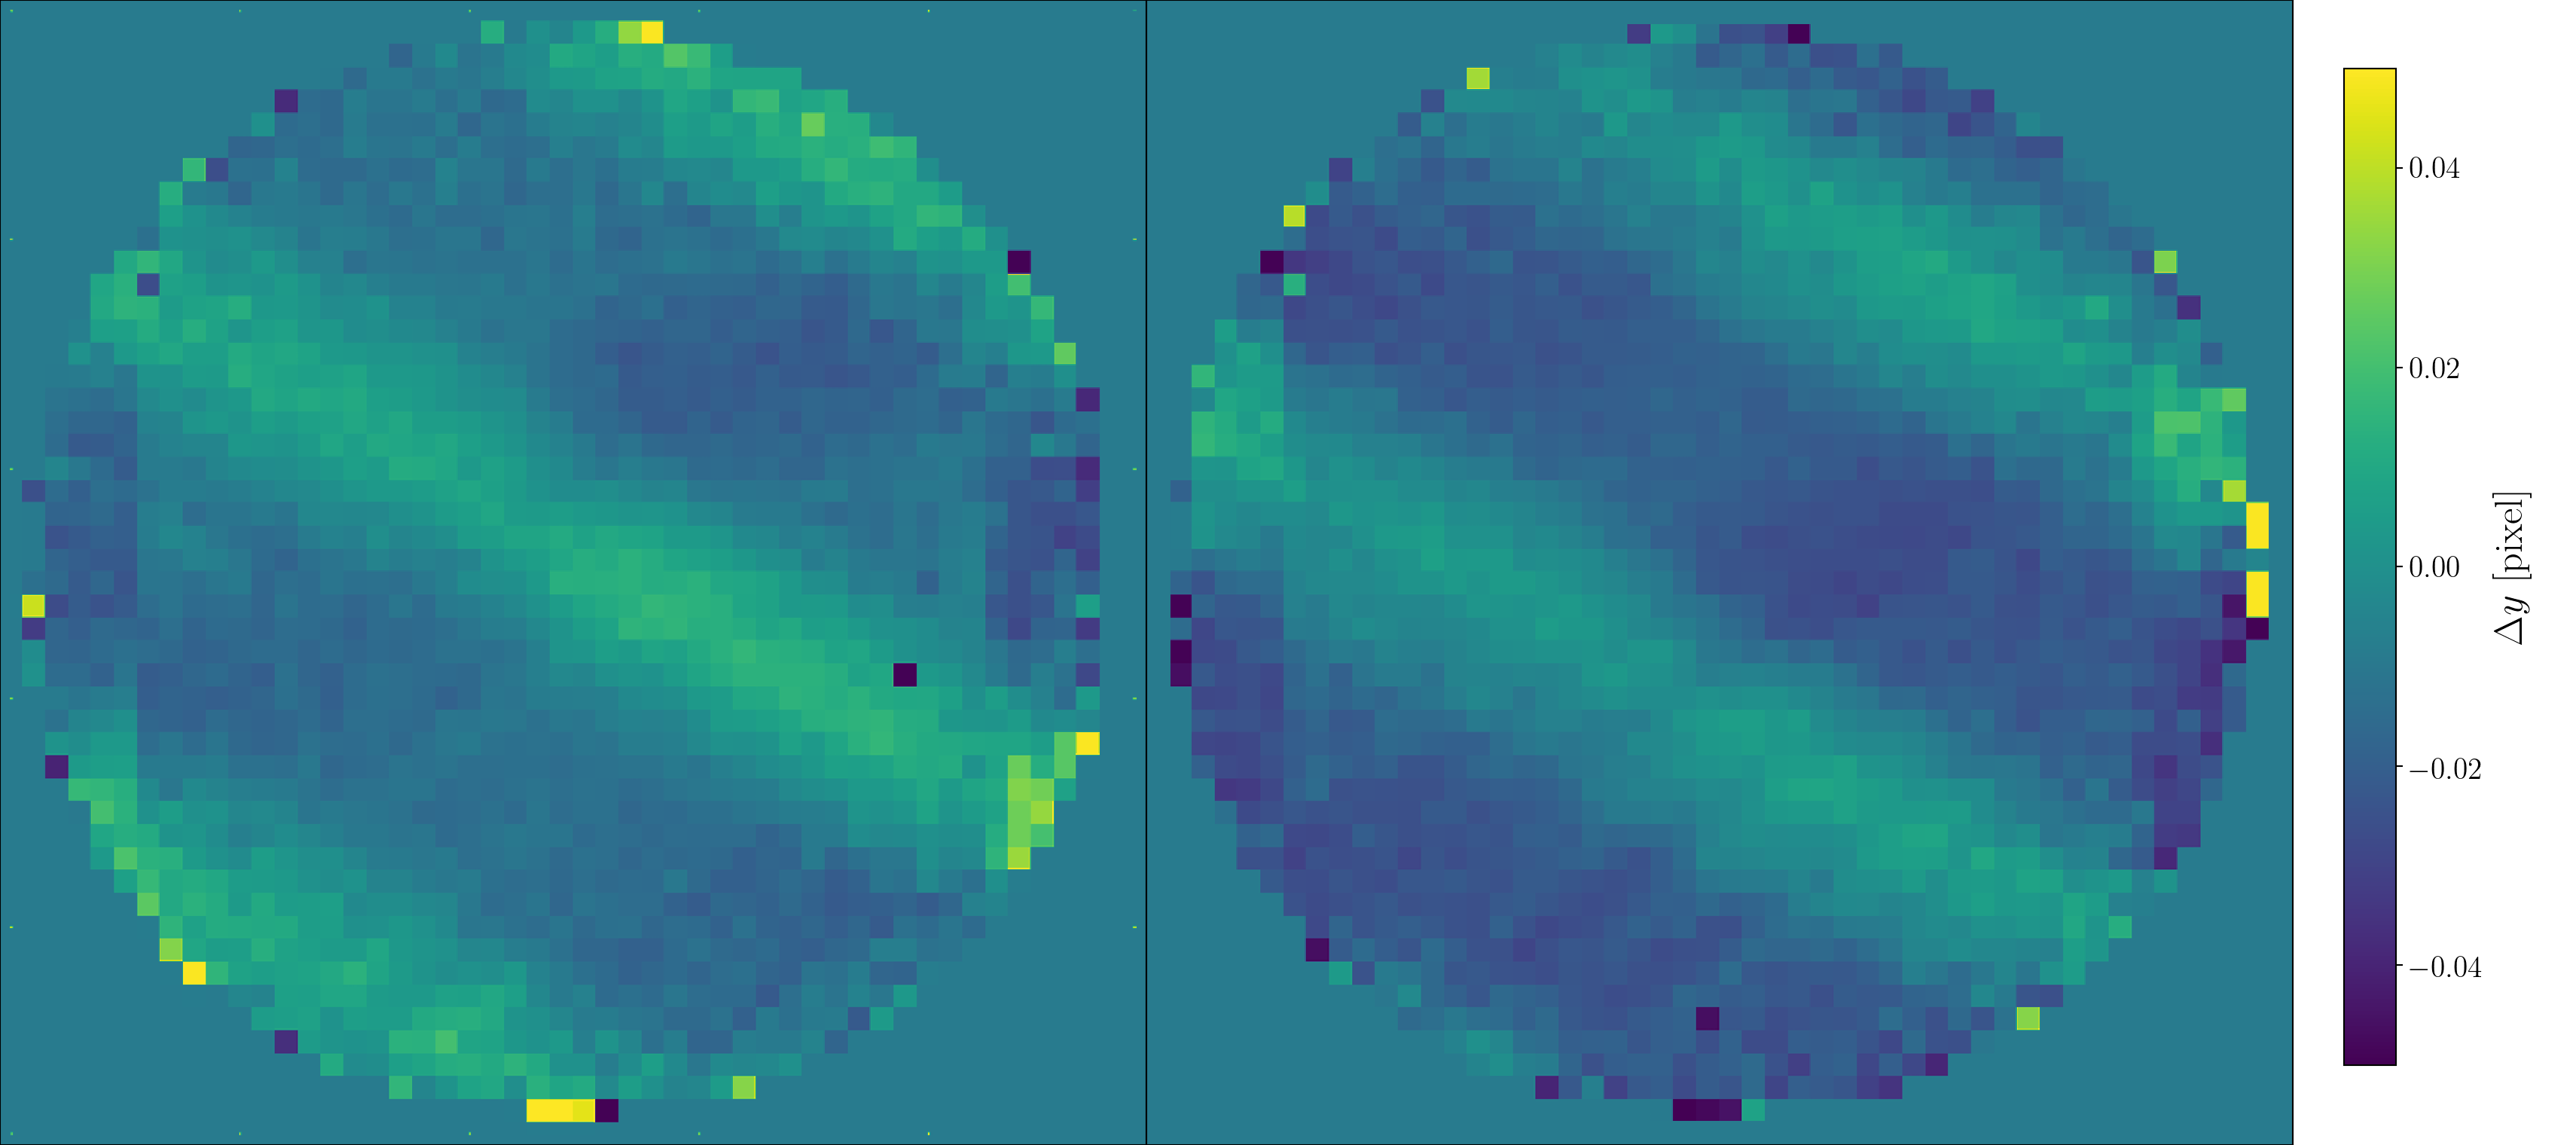
\includegraphics[width=0.6\textwidth]{figures/dif-xa-y}

\end{center}
\caption{%
  \label{distortion_xa}
  Distortion-maps of photons with different $X_A$.
  \emph{First row:} Distortion-map in x direction.
  From left to right, the $X_A$ value of photons increases.
  \emph{Second row:} Difference between distortion-maps in the first row.
  \emph{Third row:} Distortion-map in y direction.
  From left to right, the $X_A$ value of photons increases.
  \emph{Forth row:} Difference between distortion-maps in the third row.
  There is a periodic pattern in difference over the detector, which is expected to account for the phases of the coarse clock.
  }
\end{figure}

\begin{figure}[p]
\begin{center}
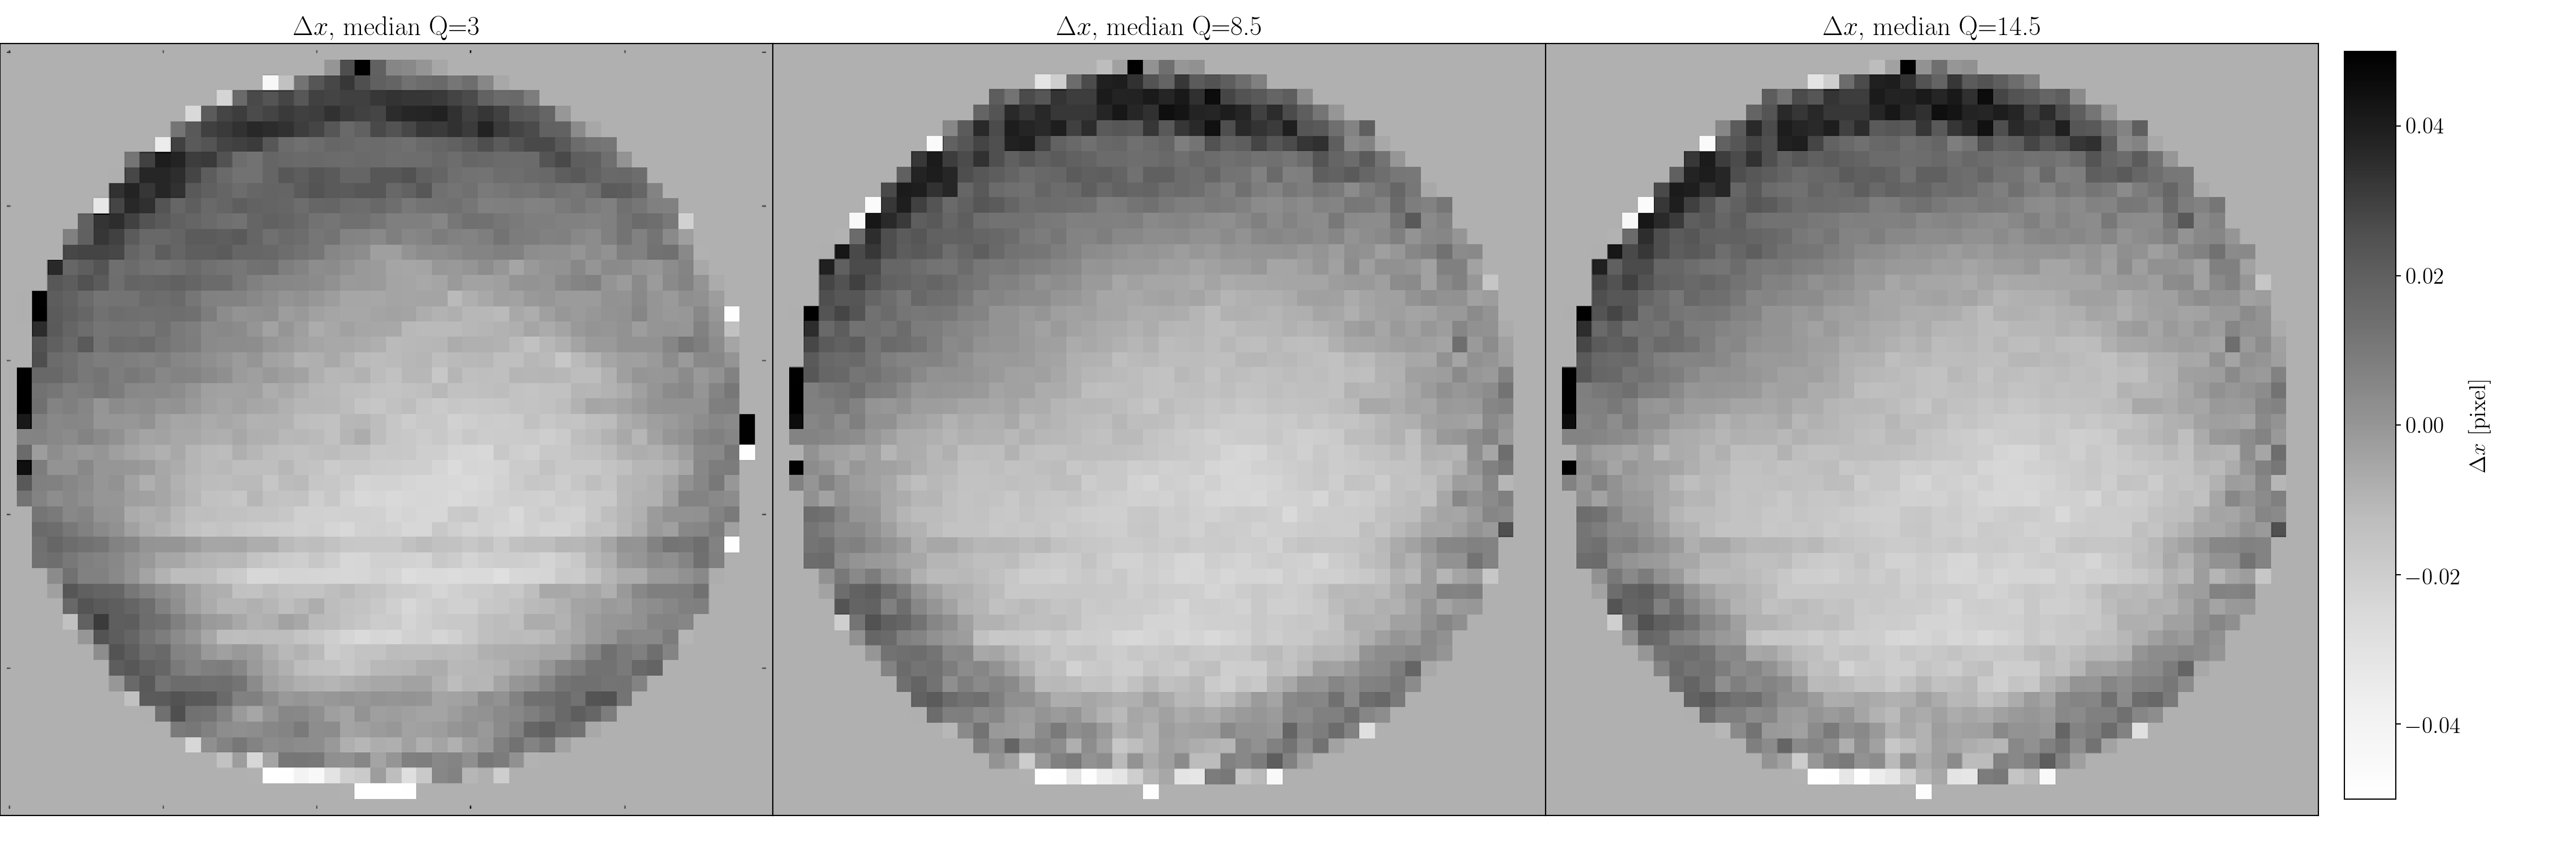
\includegraphics[width=0.95\textwidth]{figures/q-x}
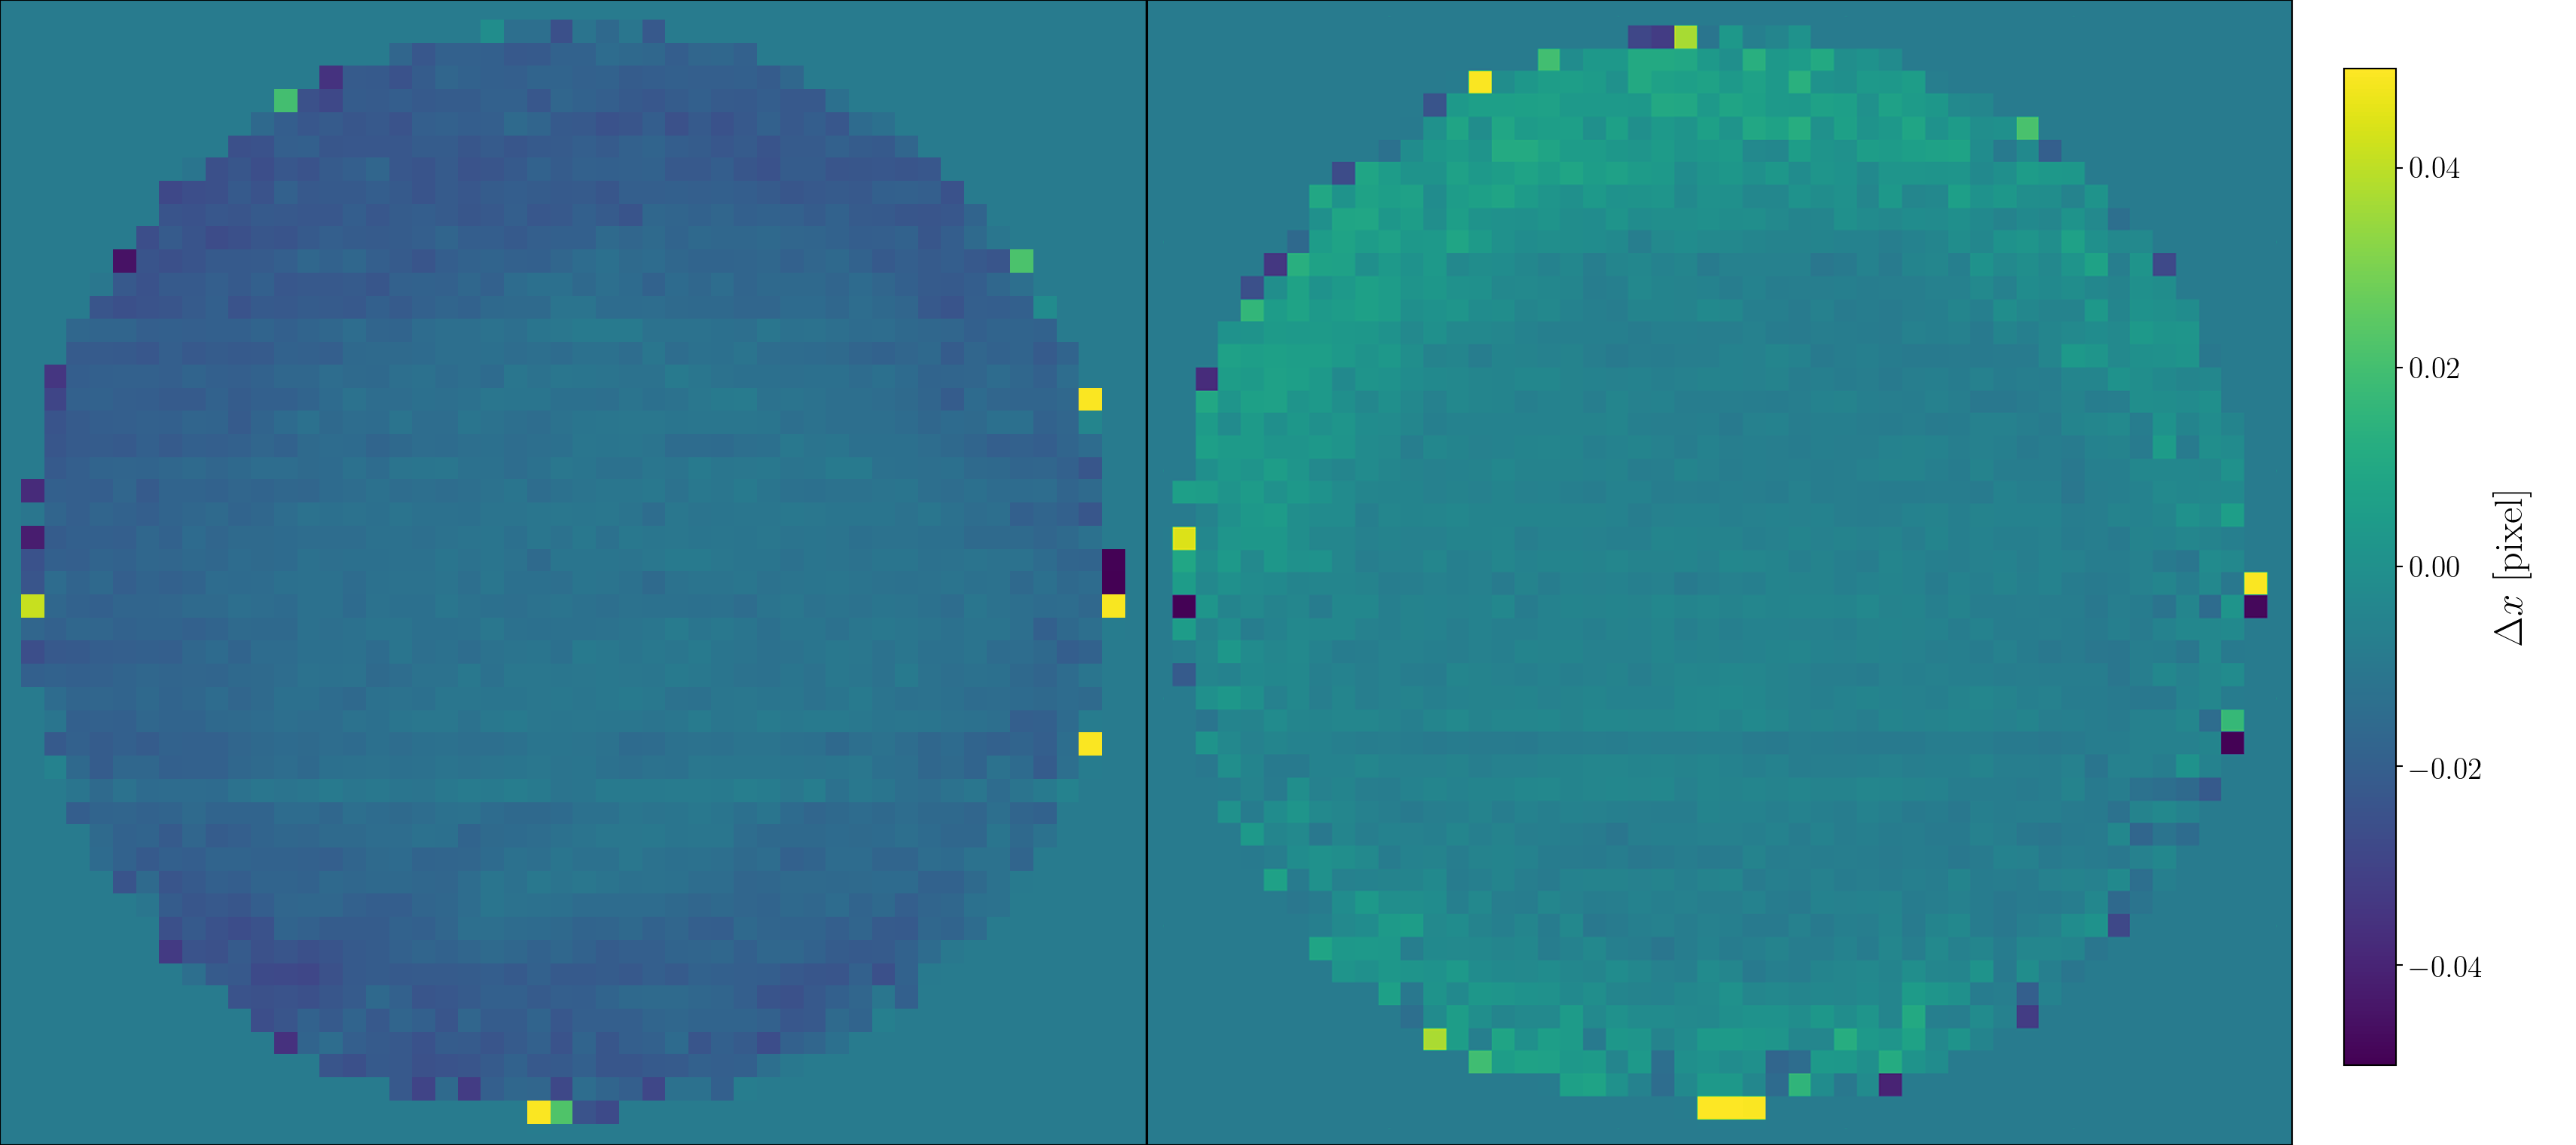
\includegraphics[width=0.6\textwidth]{figures/dif-q-x}
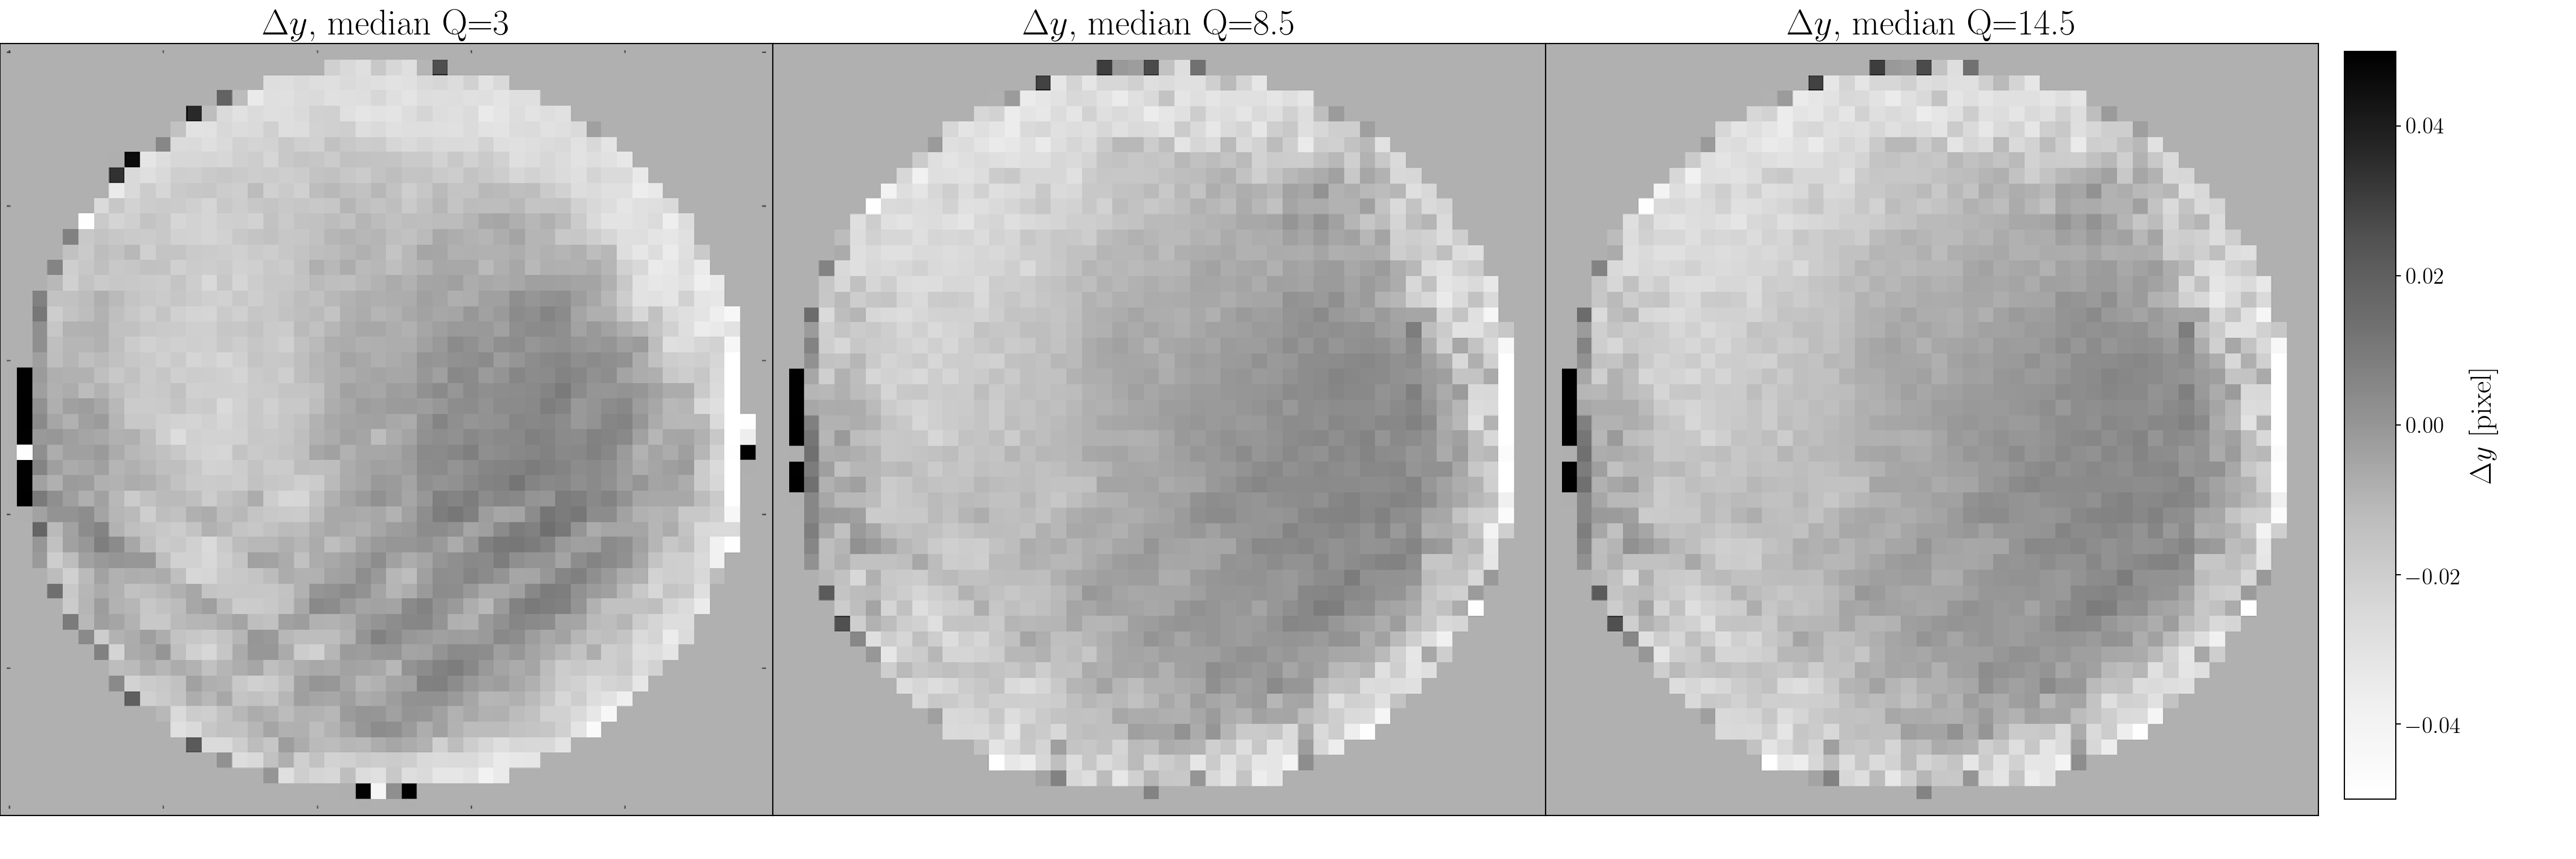
\includegraphics[width=0.95\textwidth]{figures/q-y}
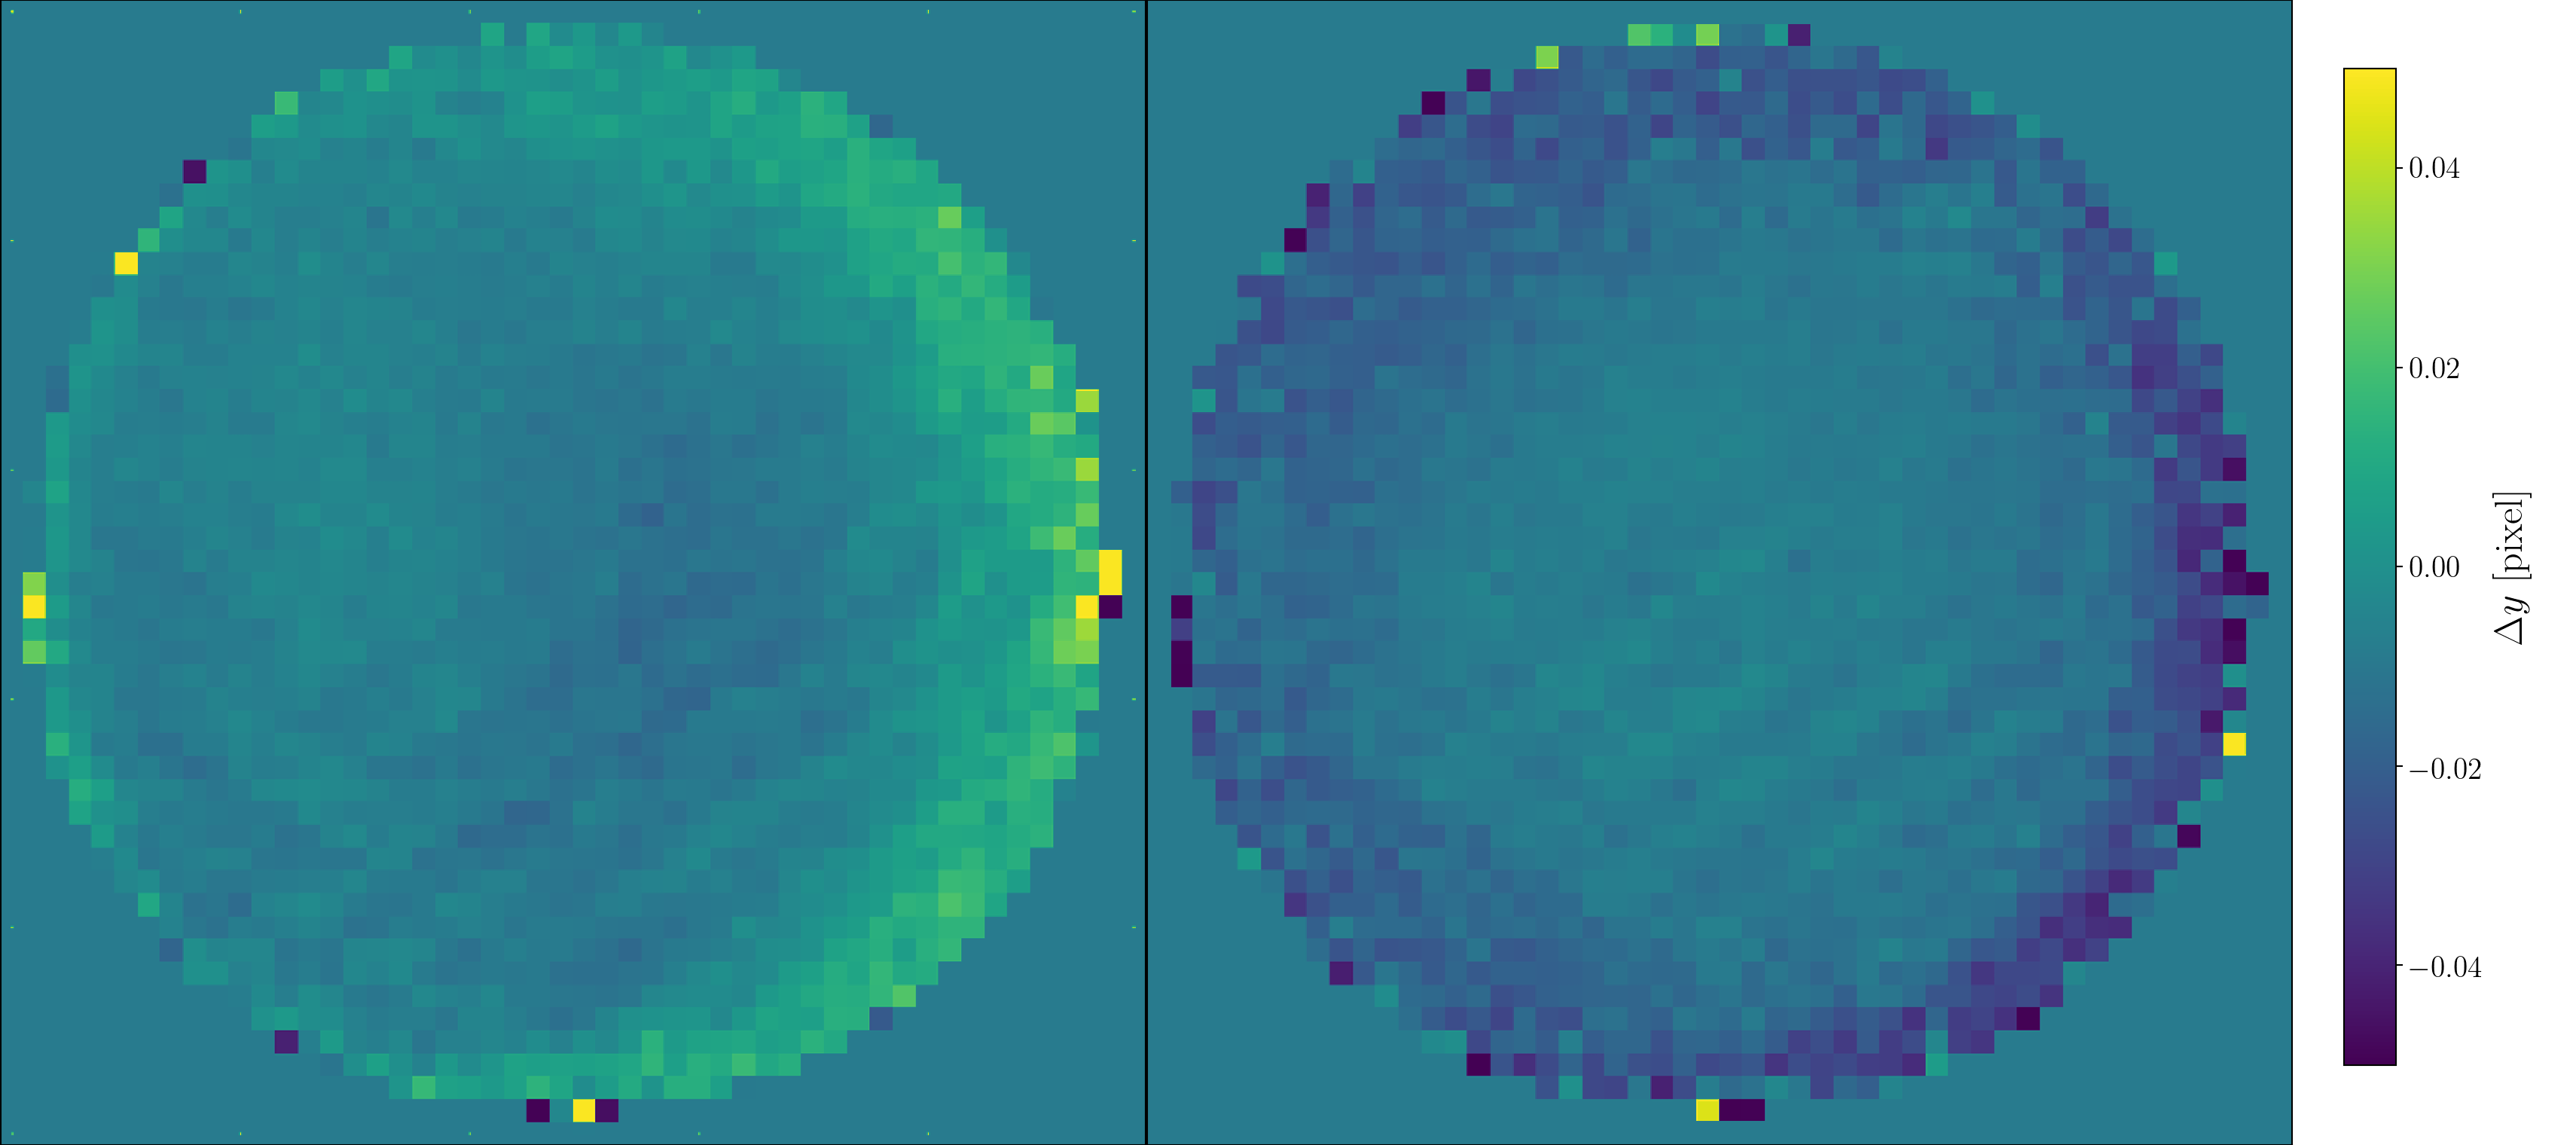
\includegraphics[width=0.6\textwidth]{figures/dif-q-y}

\end{center}
\caption{%
  \label{distortion_q}
  Distortion-maps of photons with different Q.
  \emph{First row:} Distortion-maps in x direction. 
  From left to right, the Q value of photons increases.
  \emph{Second row:} Difference between distortion-maps in the first row.
  \emph{Third row:} Distortion-map in y direction.
  From left to right, the Q value of photons increases.
  \emph{Forth row:} Difference between distortion-maps in the third row.
  }
\end{figure}


\section{Sensitivity map}
\label{sm}
To precisely construct the intensity map, the effective exposure time needs to be measured. 
Since the response function of the detector is not uniform, the sensitivity map is required to scale the effective exposure time for different pixels.
The original pipeline sensitivity map is not appropriate to be used in the calibration due to the following reasons:
\begin{enumerate}
\item The pipeline sensitivity map was constructed using ground measurements of the system throughput, which may not capture the finer details of the instrument response.
\item The \cause\ observation was conducted in the very late stage of the mission, so the response of detector could have changed during the telescope lifetime.
\item In this paper, the photons with $Q<=5$ are cut as described in section \ref{data}. 
However the photon Q value distribution over the detector is not uniform.
Fig.~\ref{qcut} shows the ratio of the remaining photons after the cut.
There are more photons cut around the edge than in the center of the detector, which changed the effective response correspondingly.
\end{enumerate}

Thanks to the observation strategy in \scanmode, each source samples a cord across the entire detector. 
If every star is assumed to be constant in brightness, the count of photons in pixel $(x,y)$ from star $i$, $C_{i,x,y}$ can be modelled as:
\begin{eqnarray}
C_{i,x,y} &=& I_{i}f_{x,y}T_{i,x,y}
\end{eqnarray}
where $I_{i}$ is the brightness of star $i$. 
$f_{x,y}$ is the sensitivity of pixel $(x,y)$.
$T_{i,x,y}$ is the exposure time of star $i$ at pixel $(x,y)$.

Starting from the original pipeline sensitivity map $f_{x,y}^{0}$, the sensitivity map is updated iteratively by the following equations:
\begin{eqnarray}
I_{i}^{n} &=& \frac{\sum_{x,y}C_{i,x,y}}{\sum_{x,y} f_{x,y}^{n} T_{i,x,y}} \\
f_{x,y}^{n+1} &=& \frac{\sum_{i}C_{i,x,y}}{\sum_{i} I_{i}^{n} T_{i,x,y}}
\end{eqnarray}

Fig.~\ref{flat} shows the comparison between the pipeline sensitivity map and the measured sensitivity map.
T

\begin{figure}[p]
\begin{center}
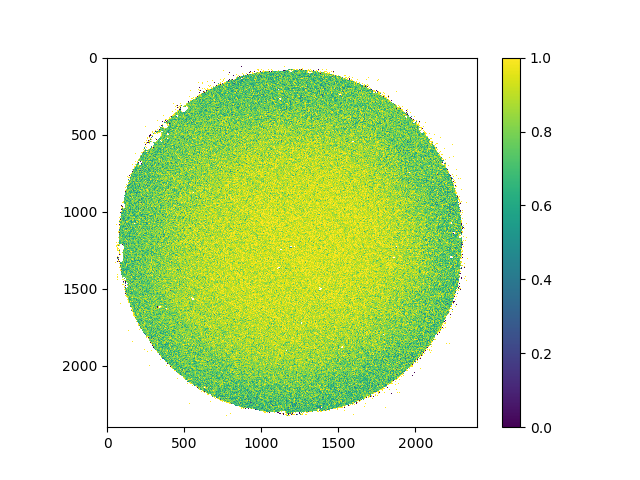
\includegraphics[width=0.8\textwidth]{figures/q50}
\end{center}
\caption{
  \label{qcut}
  The ratio of the remaining photons to the total after cutting the photons with $Q<=5$.
  There are more photons cut around the edge than in the center of the detector, which leads to a very different effective sensitivity map from the original pipeline.
}
\end{figure}

\begin{figure}[p]
\begin{center}
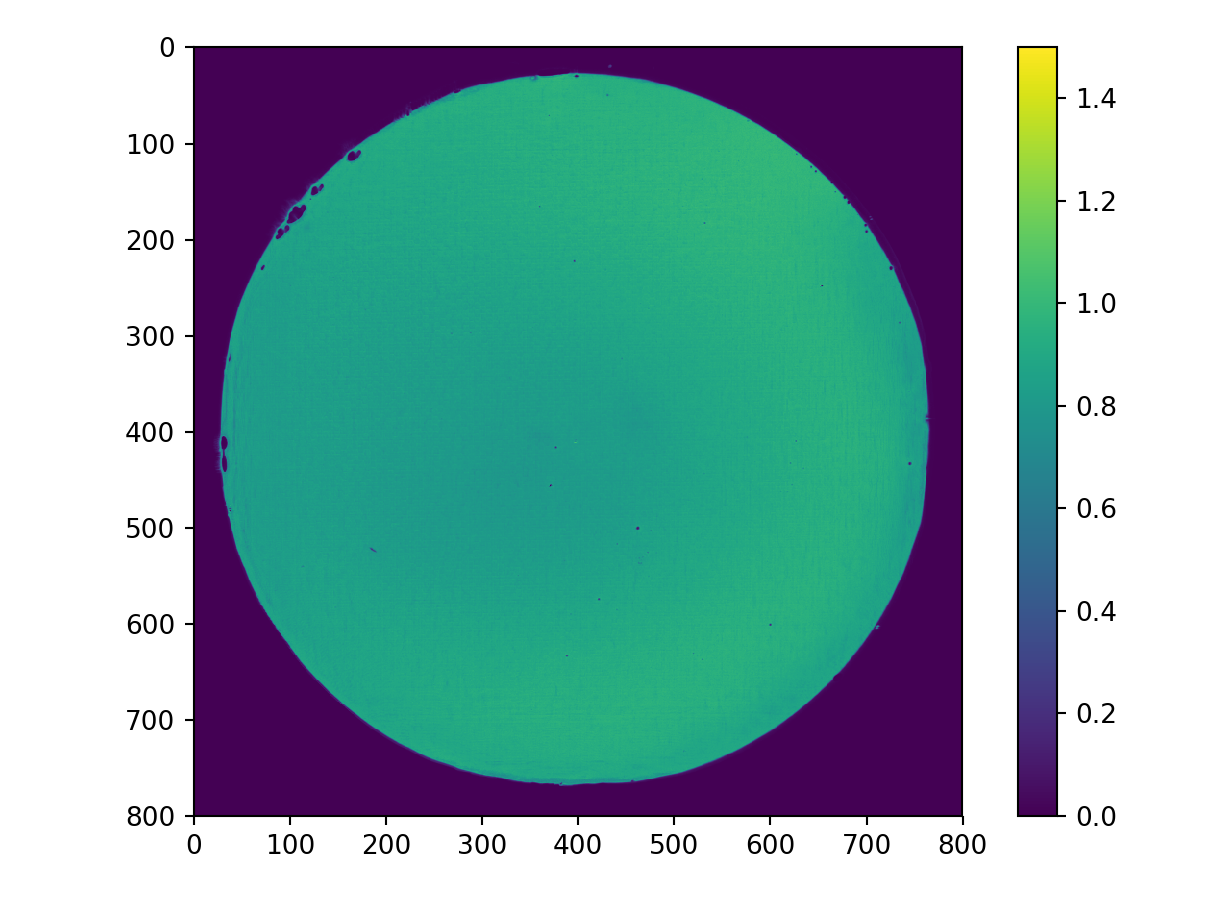
\includegraphics[width=0.48\textwidth]{figures/flato}
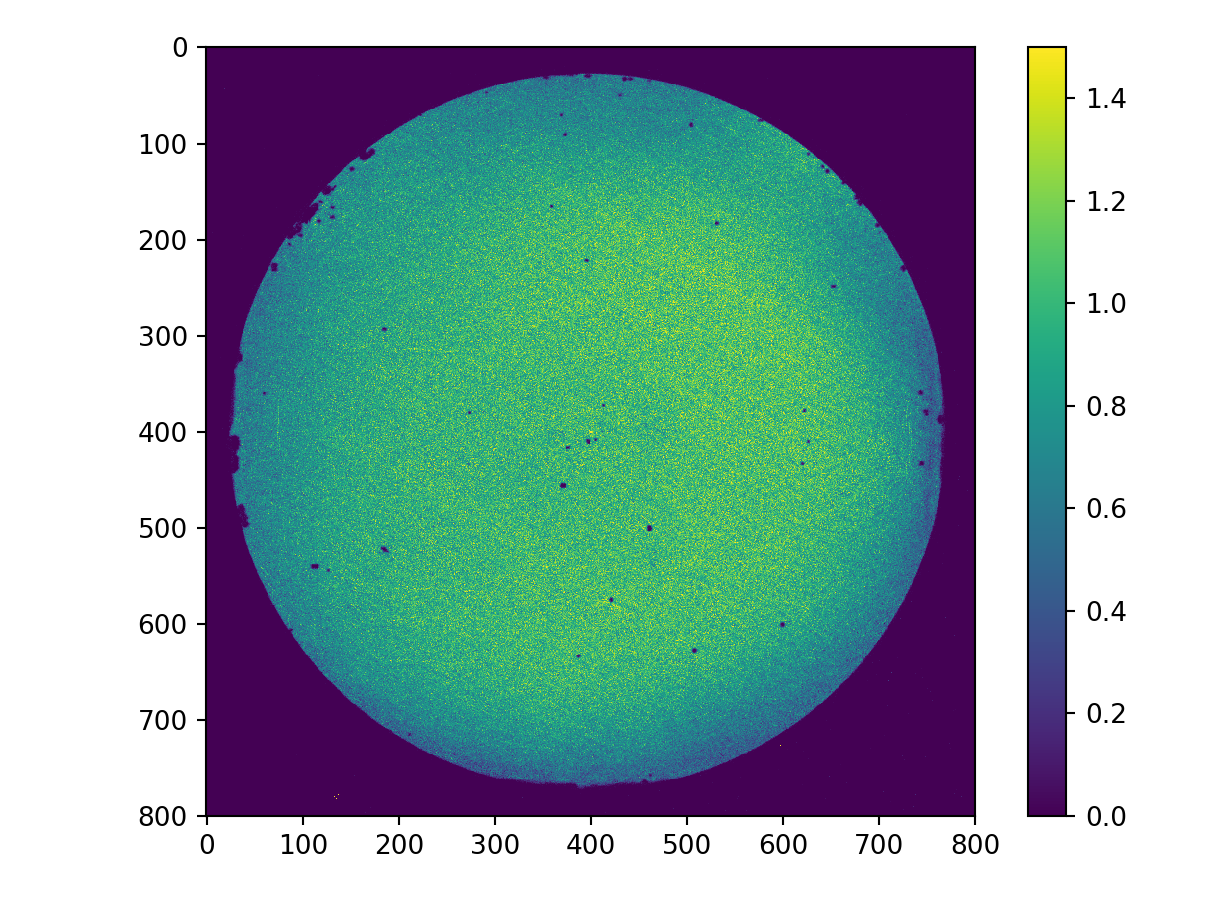
\includegraphics[width=0.48\textwidth]{figures/flat}
\end{center}
\caption{
  \label{flat}
  Comparison between measured and pipeline sensitivity map.
  \emph{Left:} Pipeline sensitivity map;
  \emph{Right:} The converged sensitivity map.
  The measured sensitivity map reproduced some of the bad spots in the original map, while has an overall lower response on the edge, which is due to the cut of the photon list.
}
\end{figure}

\begin{figure}[p]
\begin{center}
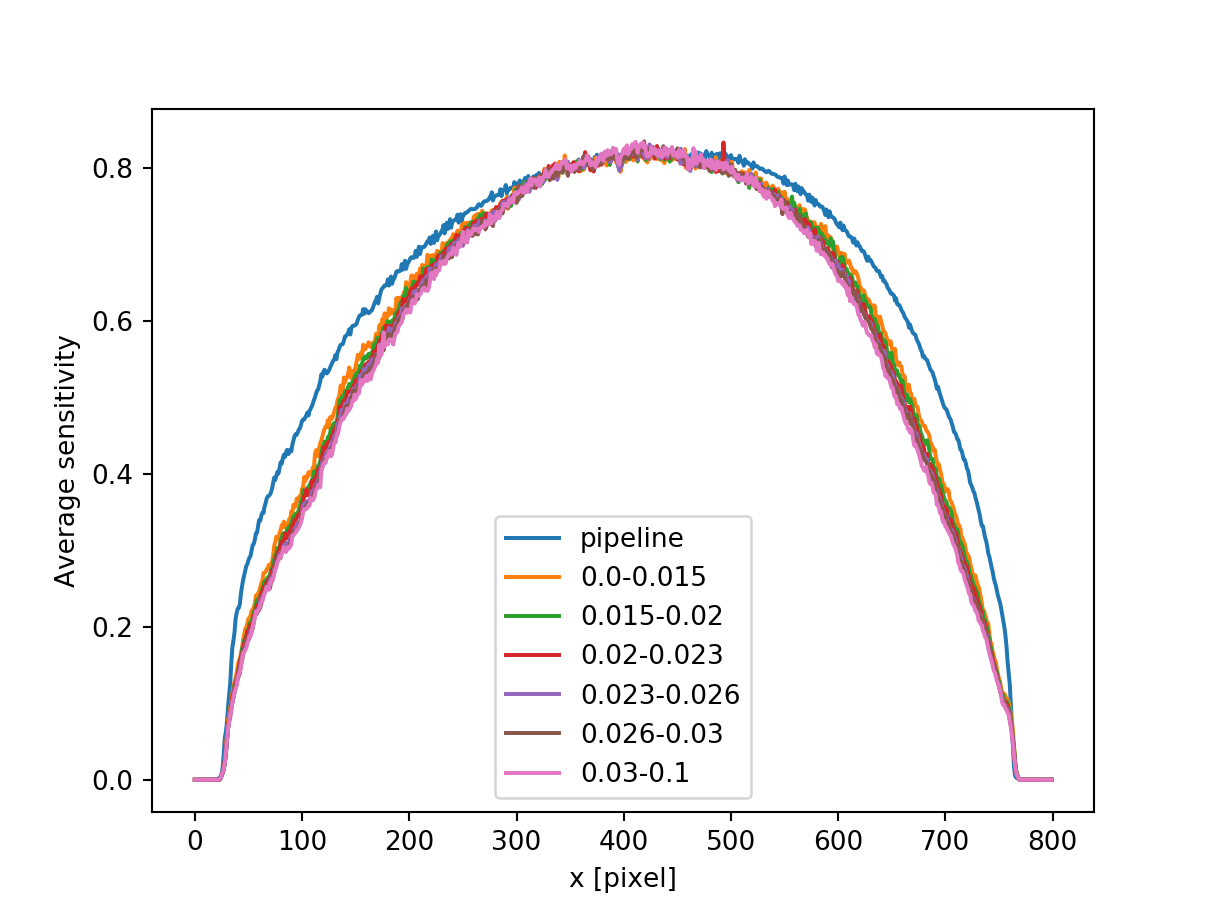
\includegraphics[width=0.48\textwidth]{figures/profile_x}
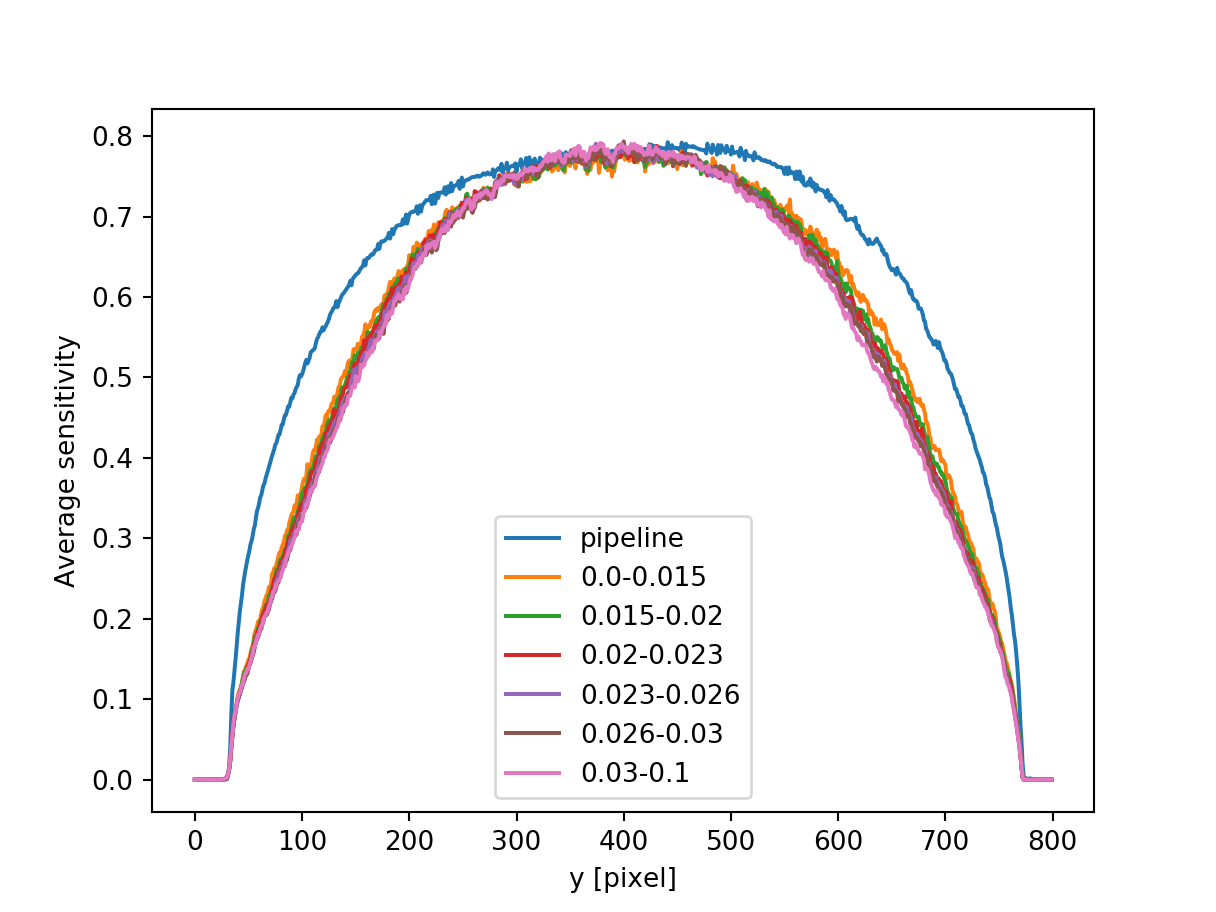
\includegraphics[width=0.48\textwidth]{figures/profile_y}
\end{center}
\caption{
  \label{flat-field}
  \emph{Left:} Profile plots of sensitivity maps in x direction;
  \emph{Right:} Profile plots of sensitivity maps in y direction.
  6 sensitivty maps are constructed by photons from regions with different photon countrate, which are compared with the pipeline sensitivity map.
}
\end{figure}


\section{Galactic plane maps}
\label{maps}
After the aspect solution, distortion map and sensitivity map are calibrated.
The corrected photon data are projected and binned into images as count maps with gnomonic projection.
To scale the effect of relative exposure time, the exposure map is constructed as:
\begin{eqnarray}
Exp(X,Y) &=& \int^{t}f(X(t), Y(t))(1-dead(t))(1-cut(t))dt
\end{eqnarray}
where $f(X(t), Y(t))$ is the sensitivity map measured in Section \ref{sm} and shifted to align with the image.
$dead(t)$ is the electronic dead time of the detector.
$cut(t)$ is the fraction of the photons that have been cut by $Q$ and $Y_A$ described in Section \ref{data}.
With the count maps and exposure maps, the intensity map is defined as the ratio of them.
Fig.~\ref{flowchart} shows the flowchart of our pipeline.

The full resolution (2 arcsec per pixel) maps are constructed   as $1 \times 2$ deg tiles with 1 deg overlap on each side of the image.
Then the maps are projected into low resolution (nside=2048) \project{Healpix} map.
Fig.~\ref{map0} shows the full Galactic plane divided into 4 equal-sized slices.
In Fig.~\ref{map1}, we also present zoom-in images in four interesting regions where Nebula structures reside.
To qualitatively illustrate the calibration performance in image level, Fig.~\ref{map2} shows the side-by-side comparison between the images generated from the original pipeline calibration and the calibration from this paper.
There are doubling artefact of individual sources and image-level smearing in the original pipeline images (left), which is caused by the imperfect aspect solution.
In comparison, there is no obvious artefact in the images from this paper.

To illustrate the coverage of this data set, Fig.~\ref{map3} shows the all sky Mollweide projection NUV intensity map constructed from from the \asc\ data, the \msc\ data and the \cause\ data (this paper).
The \cause\ data fill most of the sky around the Galactic Plane that have never been observed in the \galex\ main mission.
In Fig.~\ref{map4}, we present the Galactic Plane images from different surveys. 
The structure of Galactic Plane varies dramatically in different wavelength.
\begin{figure}[p]
\begin{center}
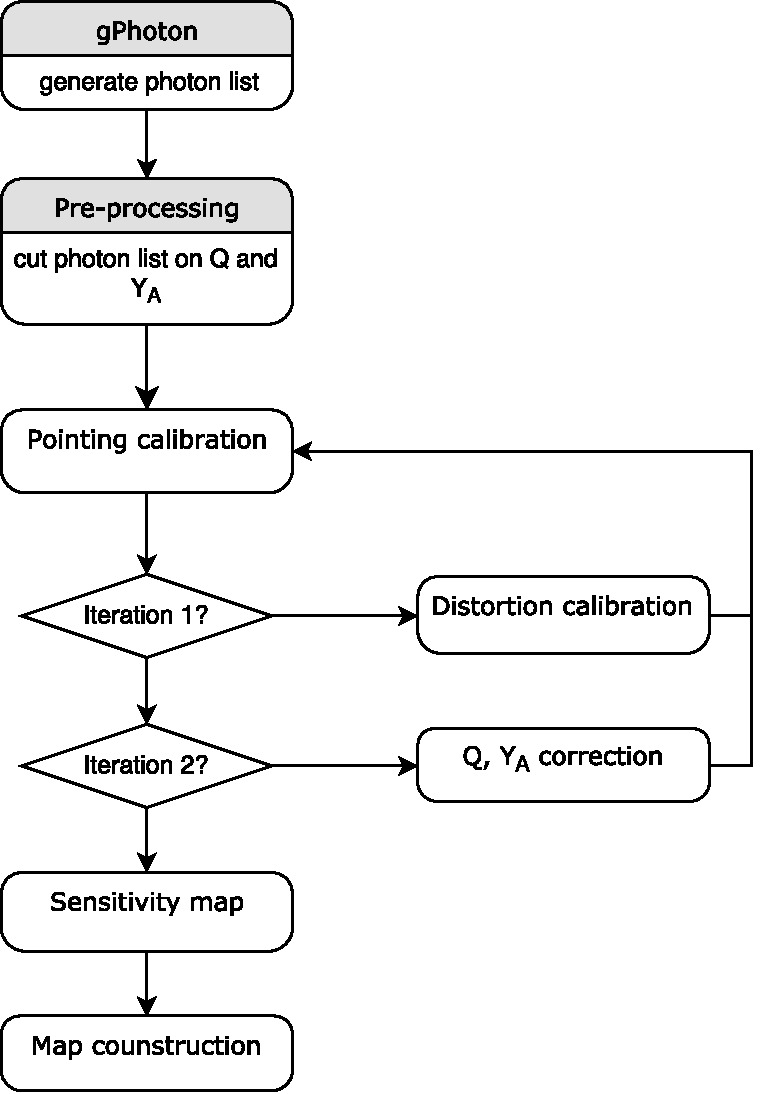
\includegraphics[width=0.6\textwidth]{figures/flowchart}
\end{center}
\caption{
  \label{flowchart}
  The flowchart of the pipeline.
}
\end{figure}


\begin{figure}[p]
\begin{center}
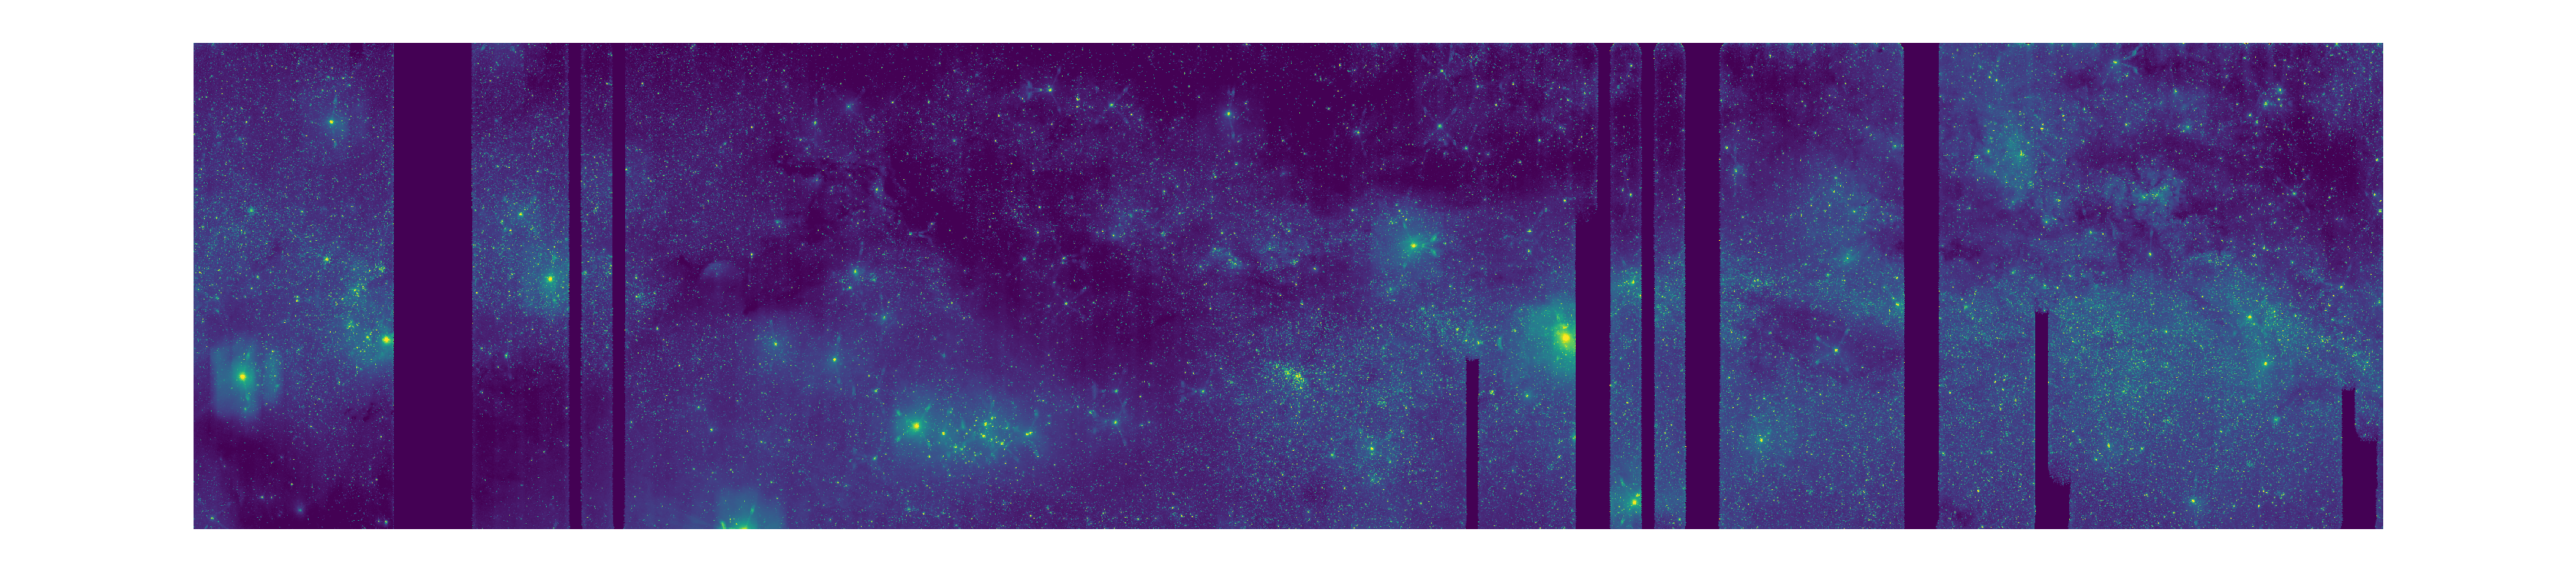
\includegraphics[width=1.\textwidth]{figures/cartview1}
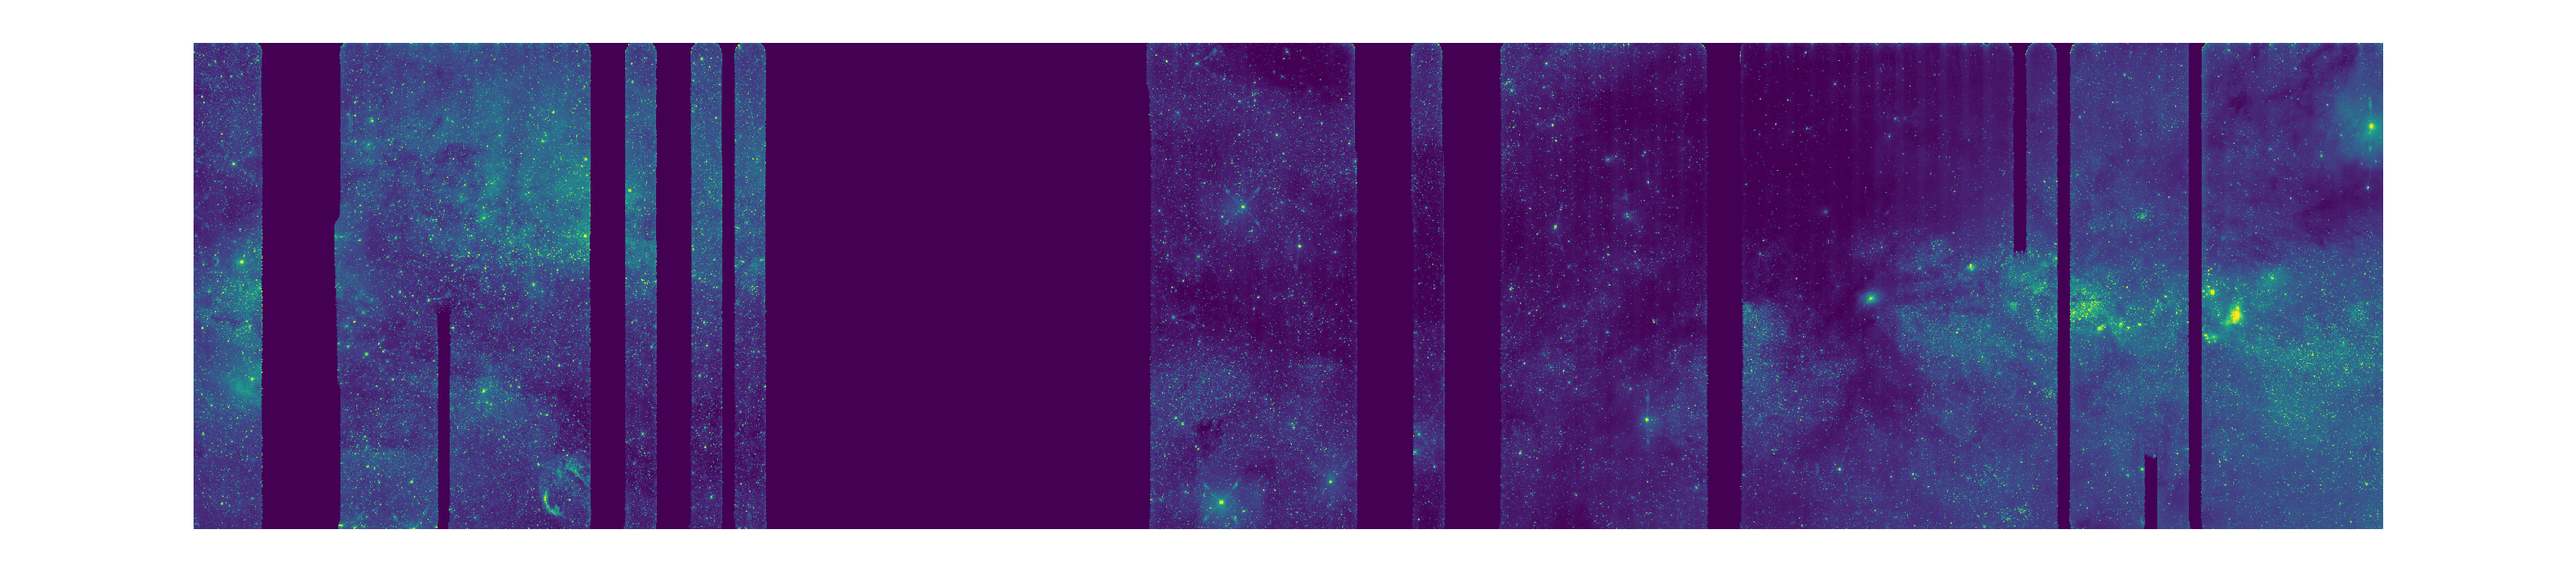
\includegraphics[width=1.\textwidth]{figures/cartview2}
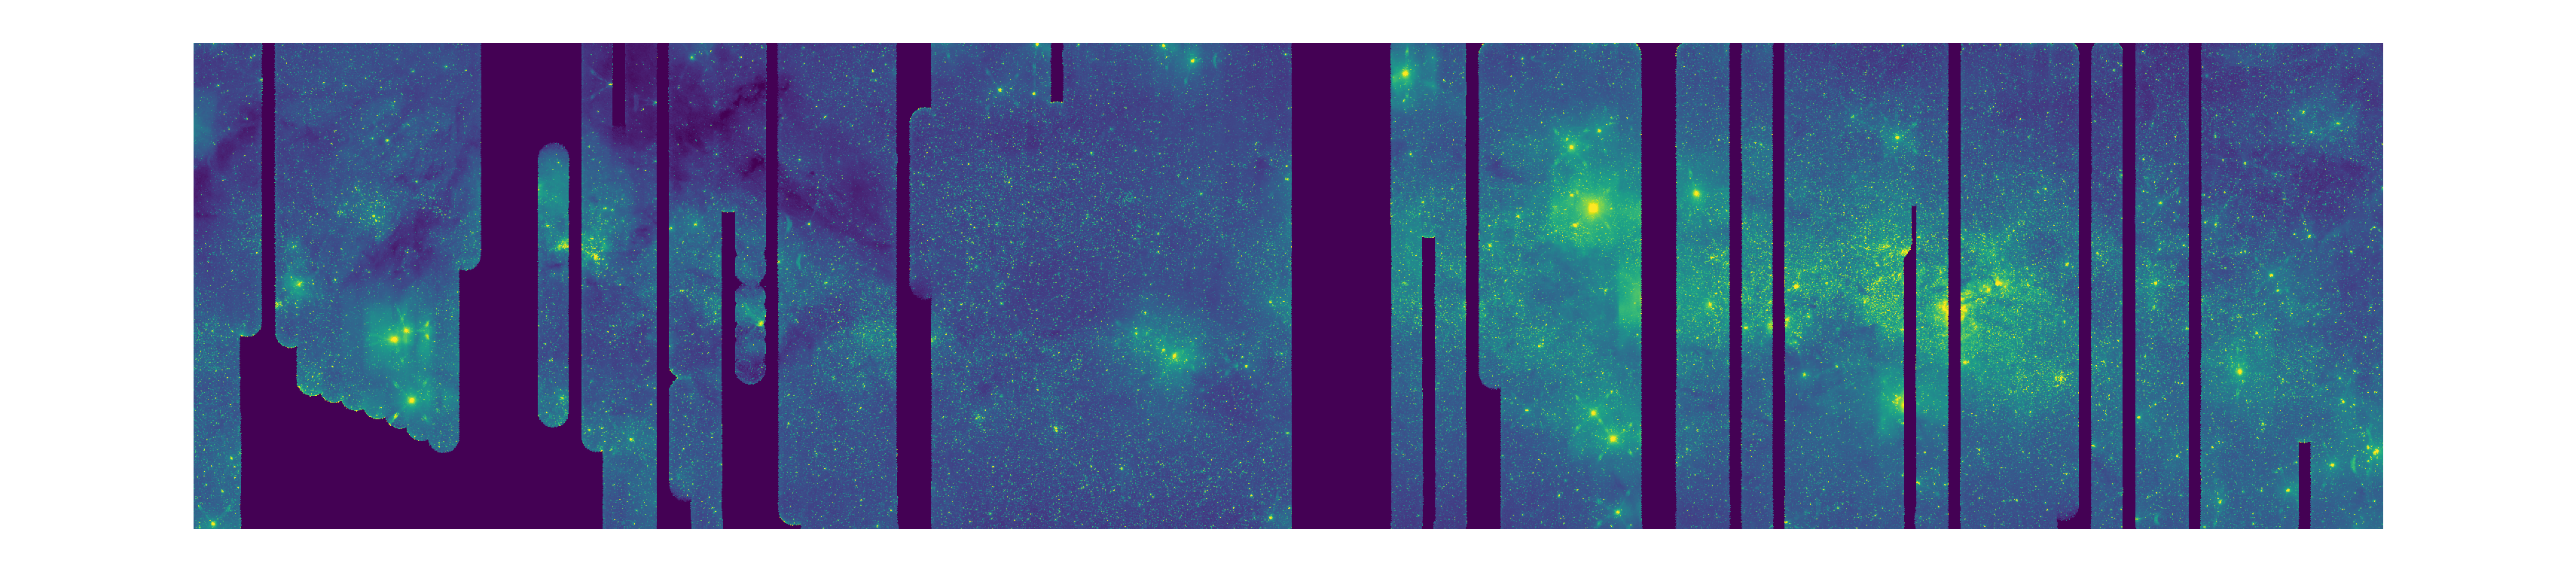
\includegraphics[width=1.\textwidth]{figures/cartview3}
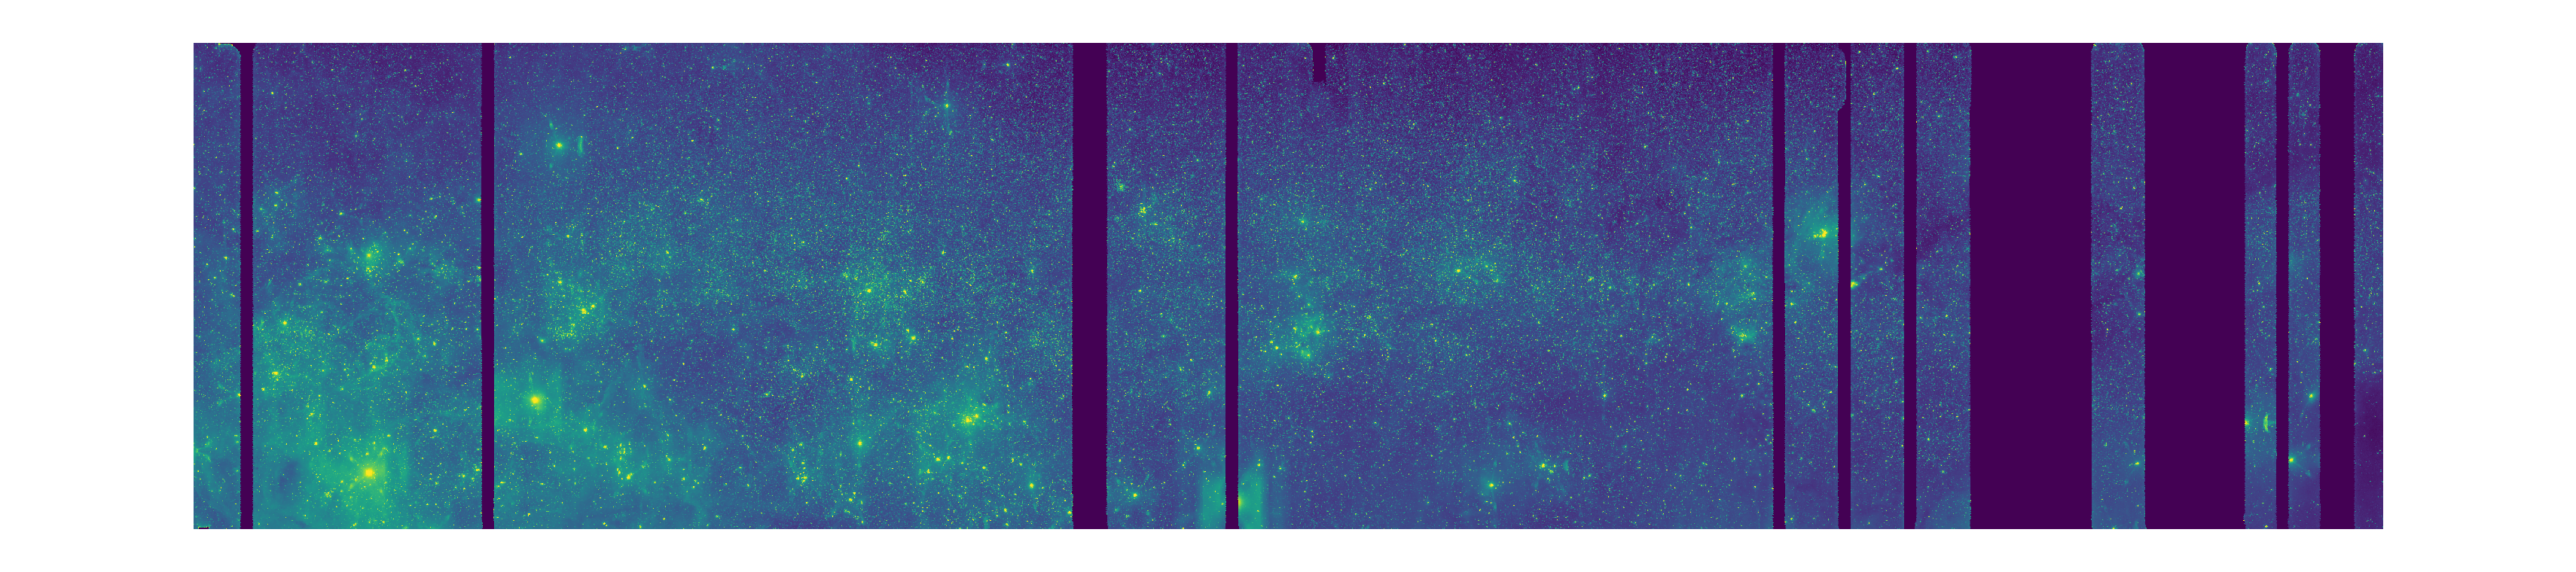
\includegraphics[width=1.\textwidth]{figures/cartview4}
\end{center}
\caption{
  \label{map0}
  Four equal-sized slice of the Galactic Plane($-10<=gb<=10$).
  From top to bottom, the ranges of Galactic longitude are: 90-180 deg, 0-90 deg, 270-360 deg and 180-270 deg.
}
\end{figure}

\begin{figure}[p]
\begin{center}
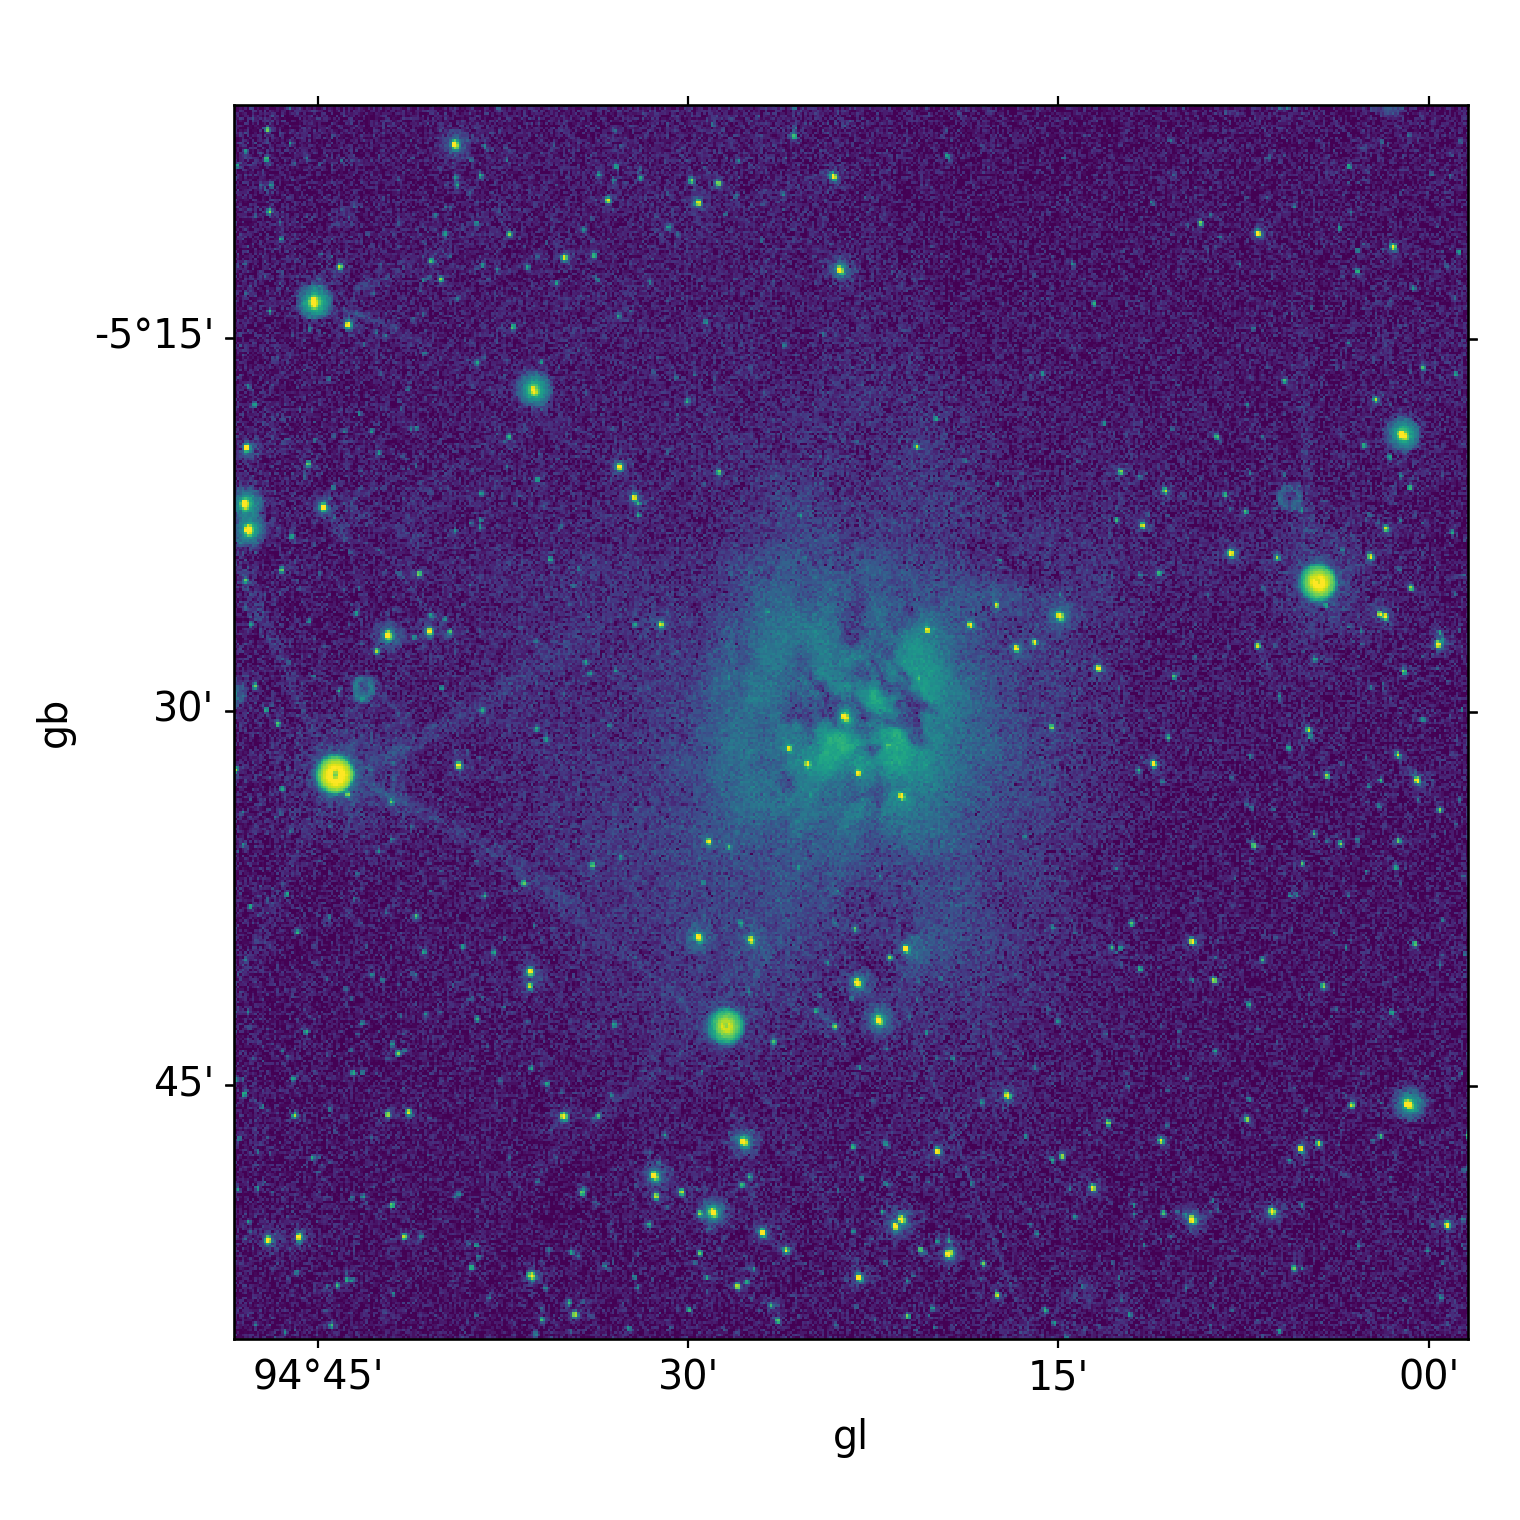
\includegraphics[width=0.49\textwidth]{figures/cocoon}
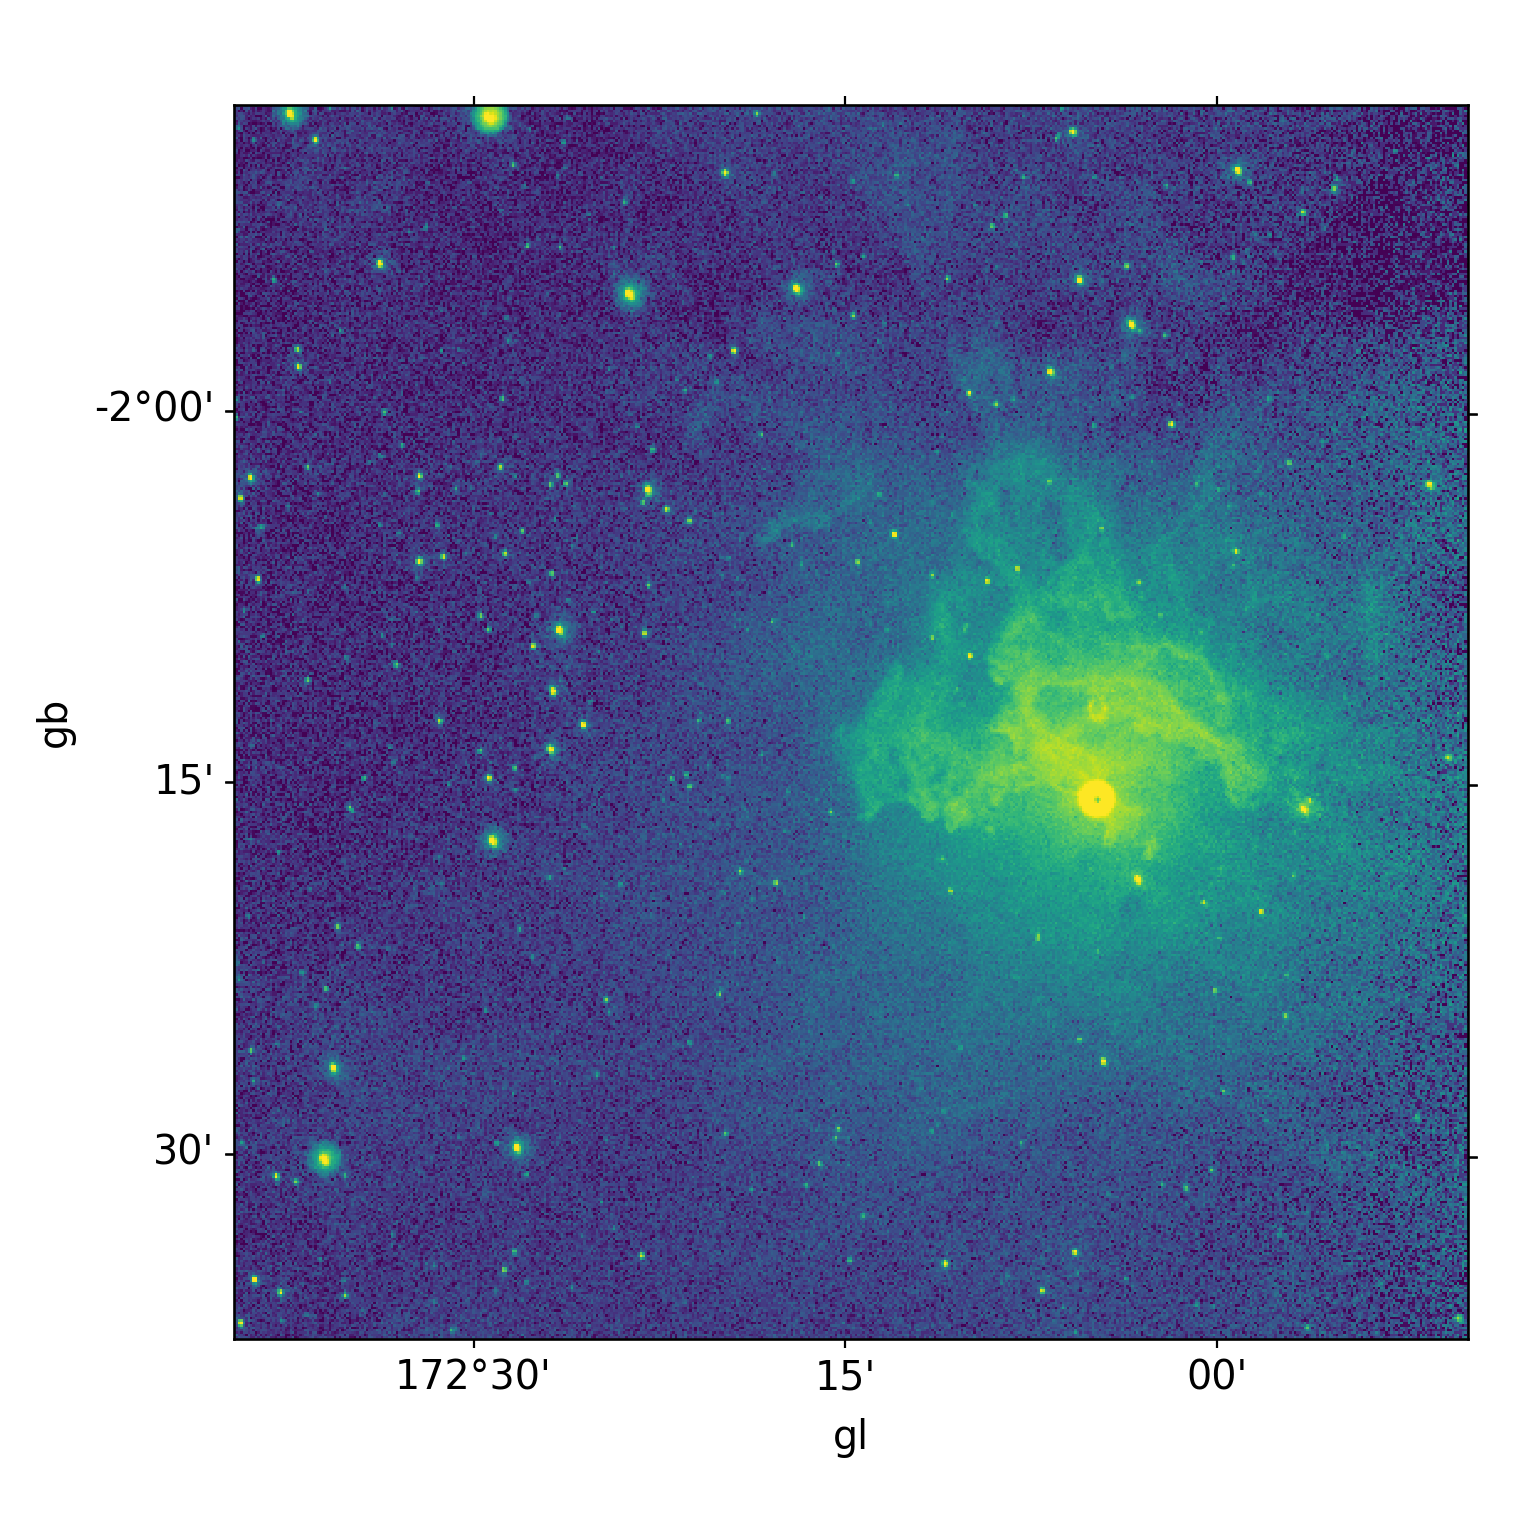
\includegraphics[width=0.49\textwidth]{figures/FlamingStar}
\includegraphics[width=0.49\textwidth]{figures/Vela}
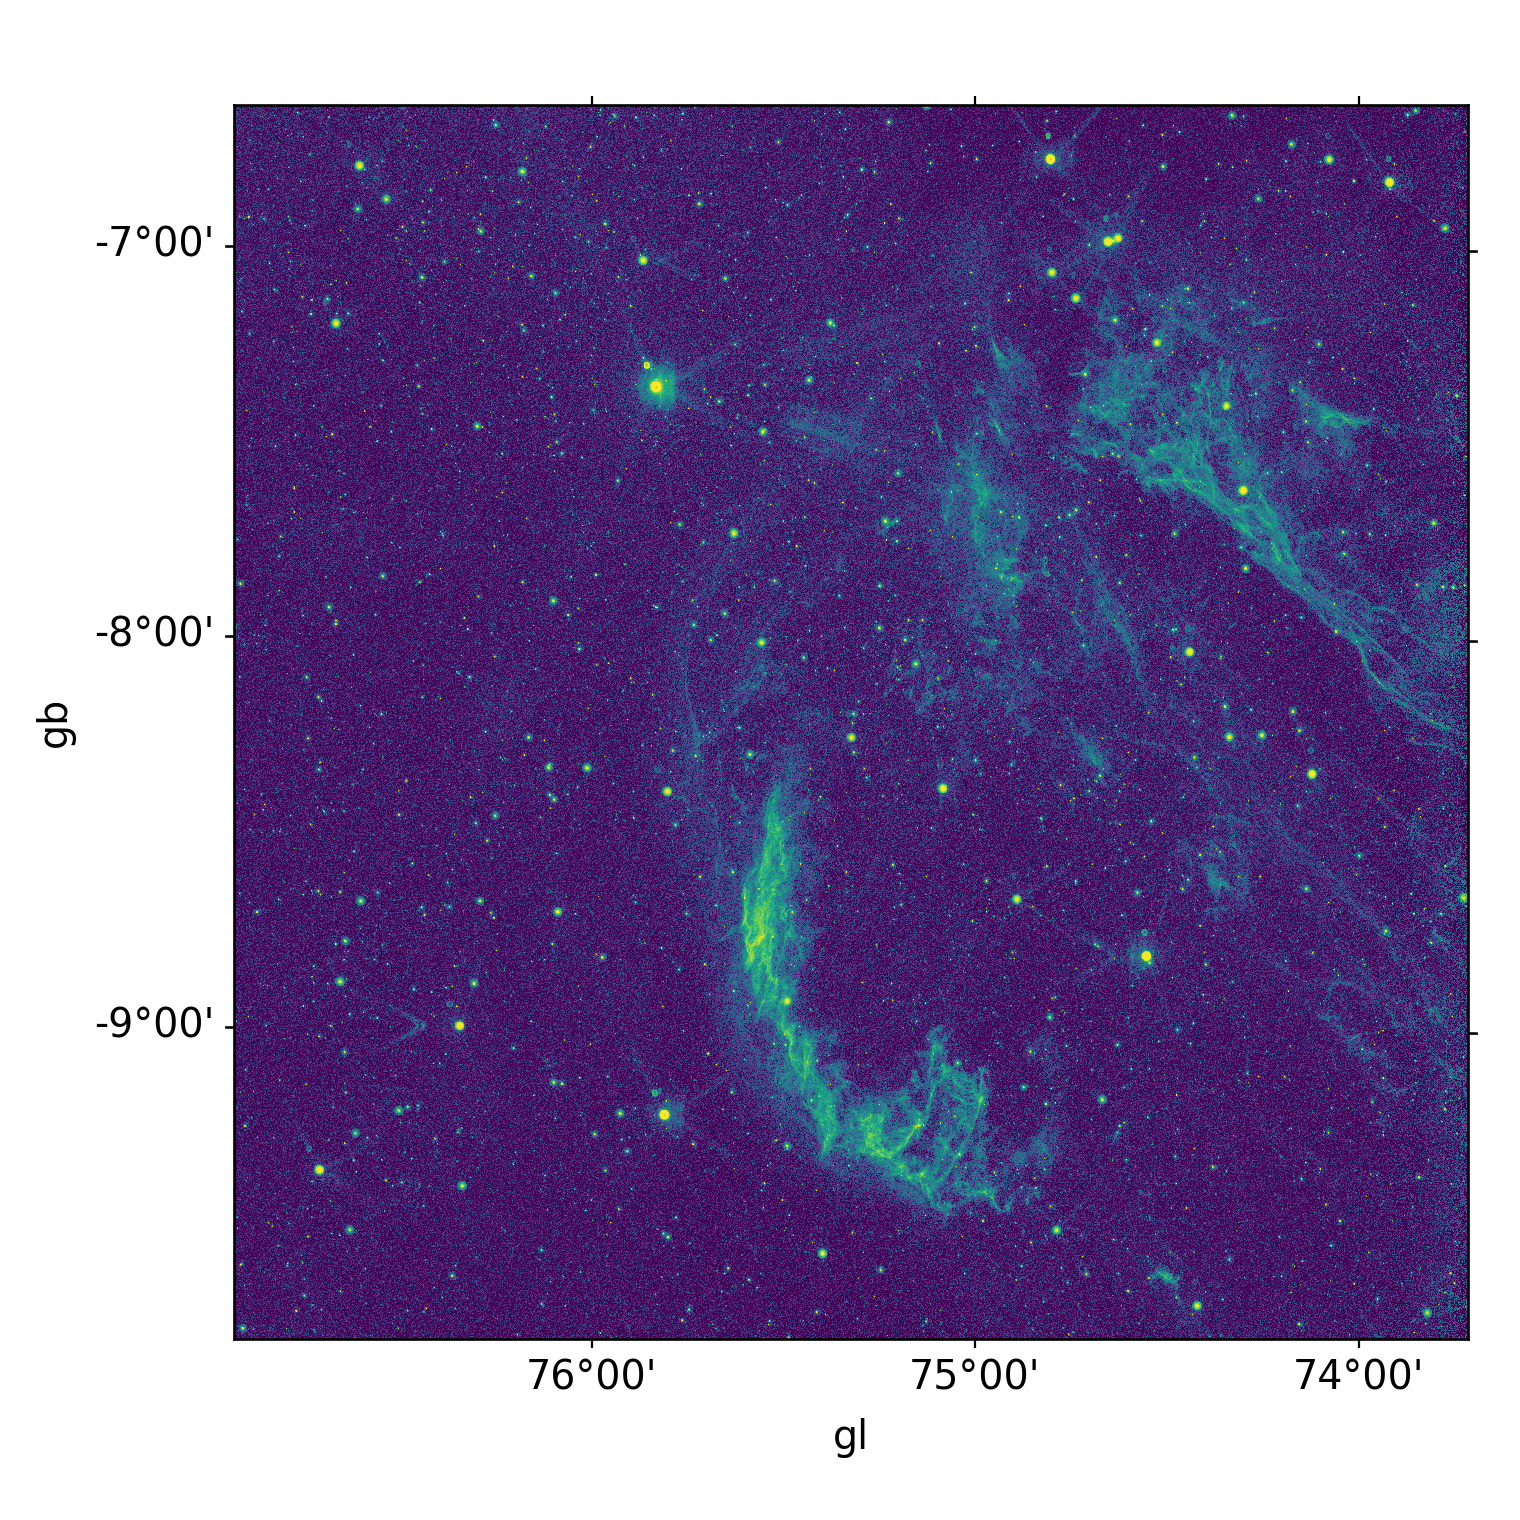
\includegraphics[width=0.49\textwidth]{figures/cygnusloop}
\end{center}
\caption{
  \label{map1}
   \emph{Top-left:}  the Cocoon Nebula;
   \emph{Top-right:} the Flaming Star Nebula;
   \emph{Bottom-left:} the Vela Supernova Remnant;
   \emph{Bottom-right:} the Cygnus Loop Nebula.
}
\end{figure}

\begin{figure}[p]
\begin{center}
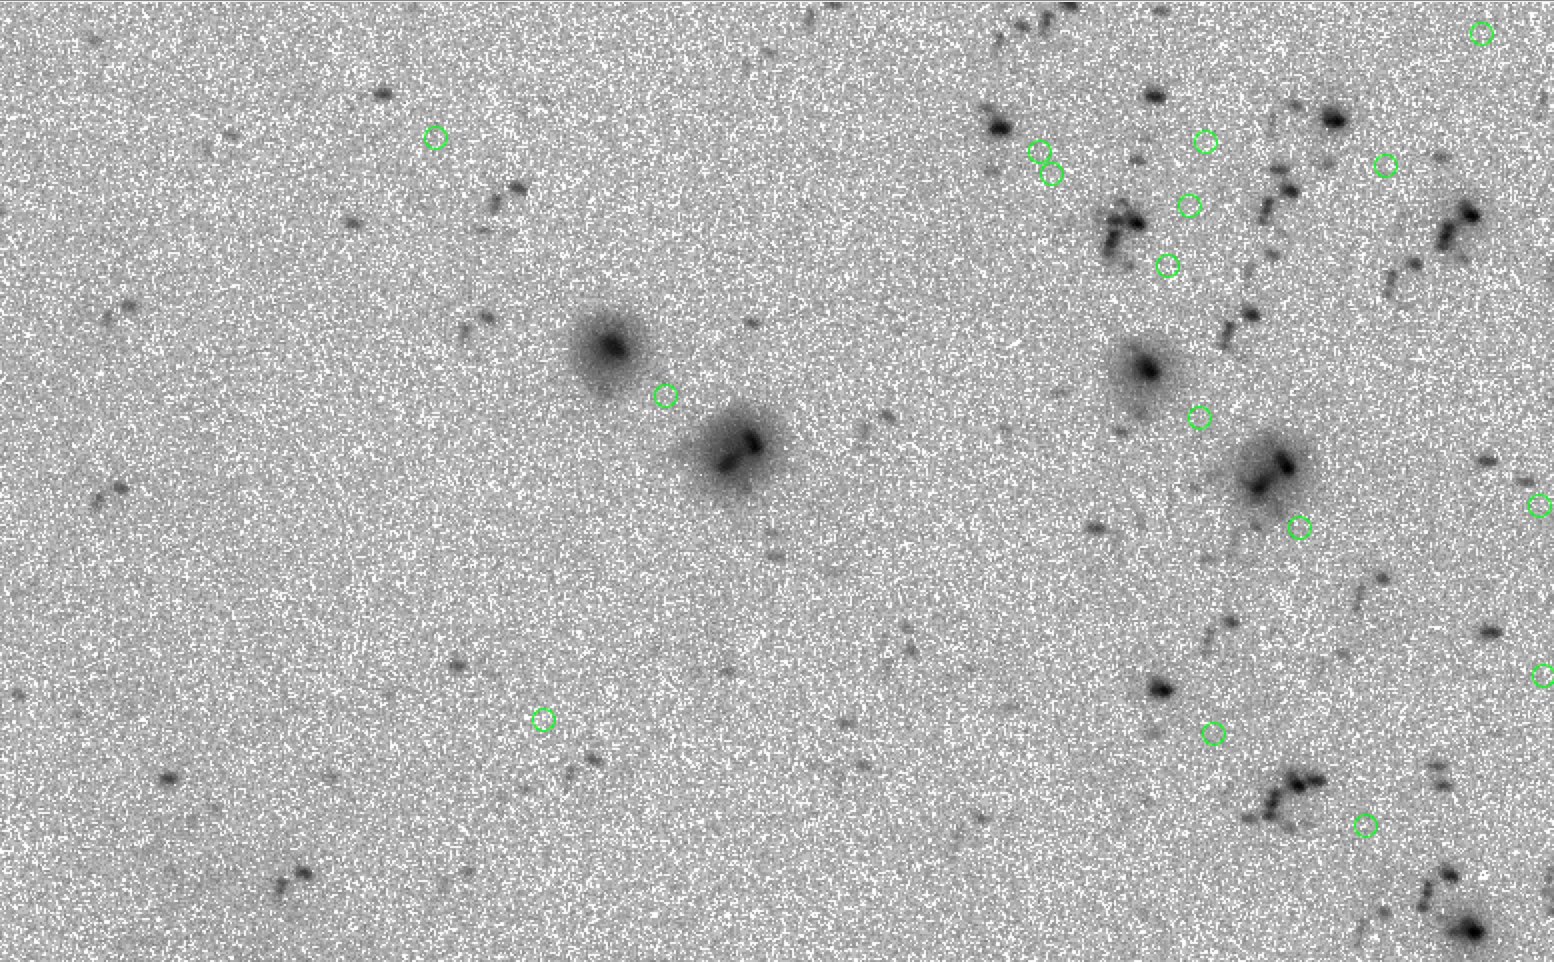
\includegraphics[width=0.49\textwidth]{figures/pip0}
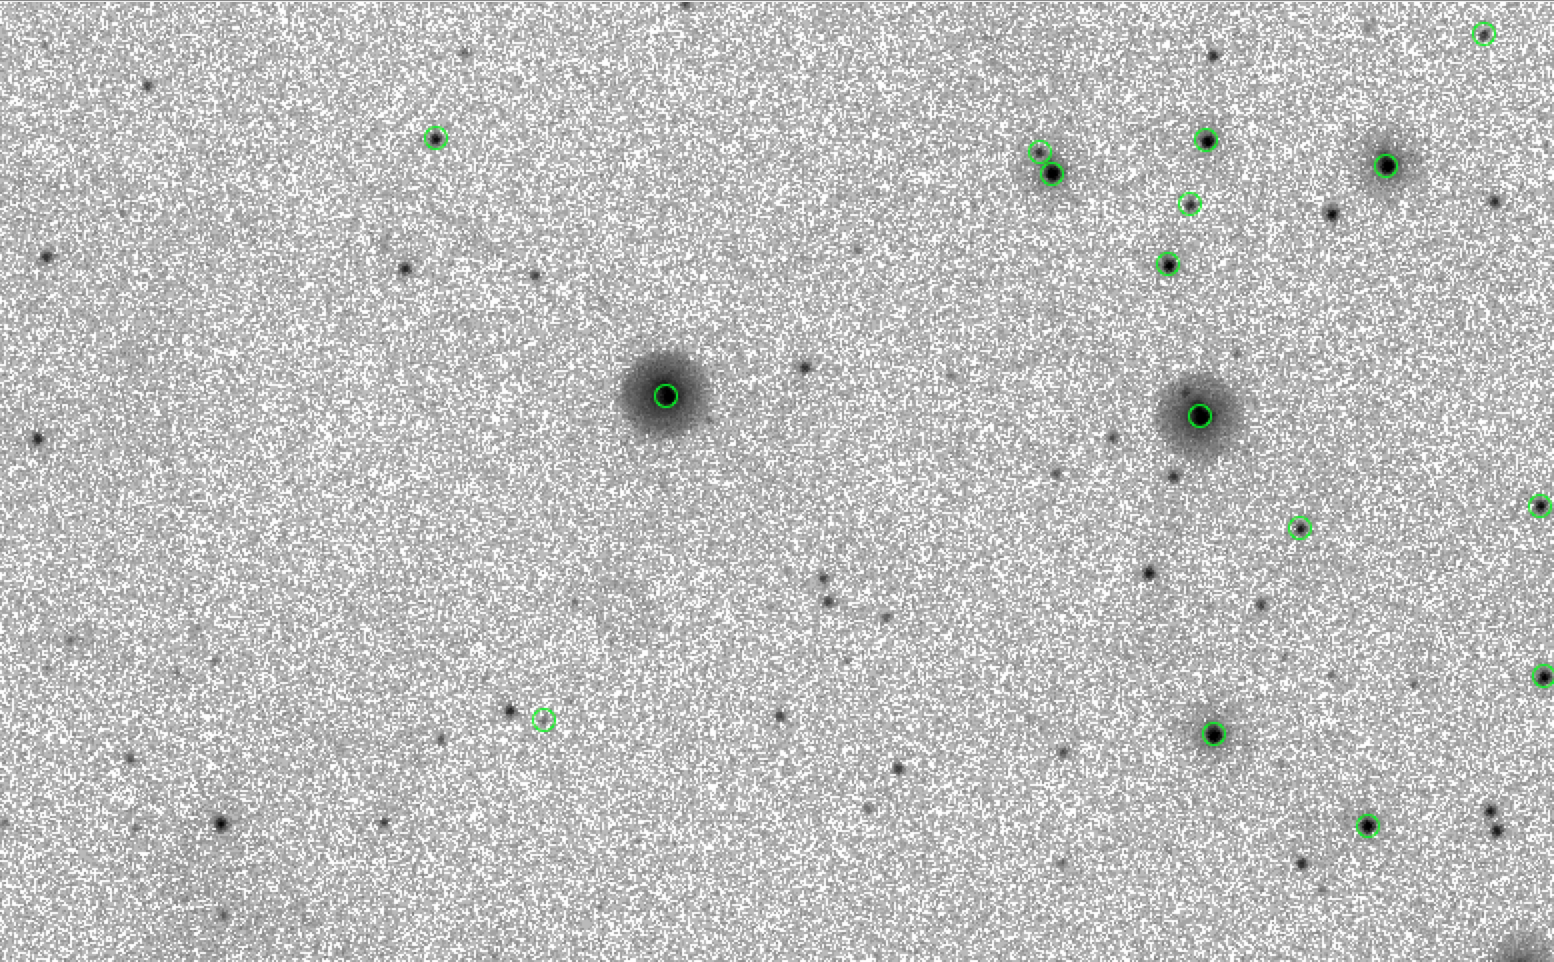
\includegraphics[width=0.49\textwidth]{figures/cal0}
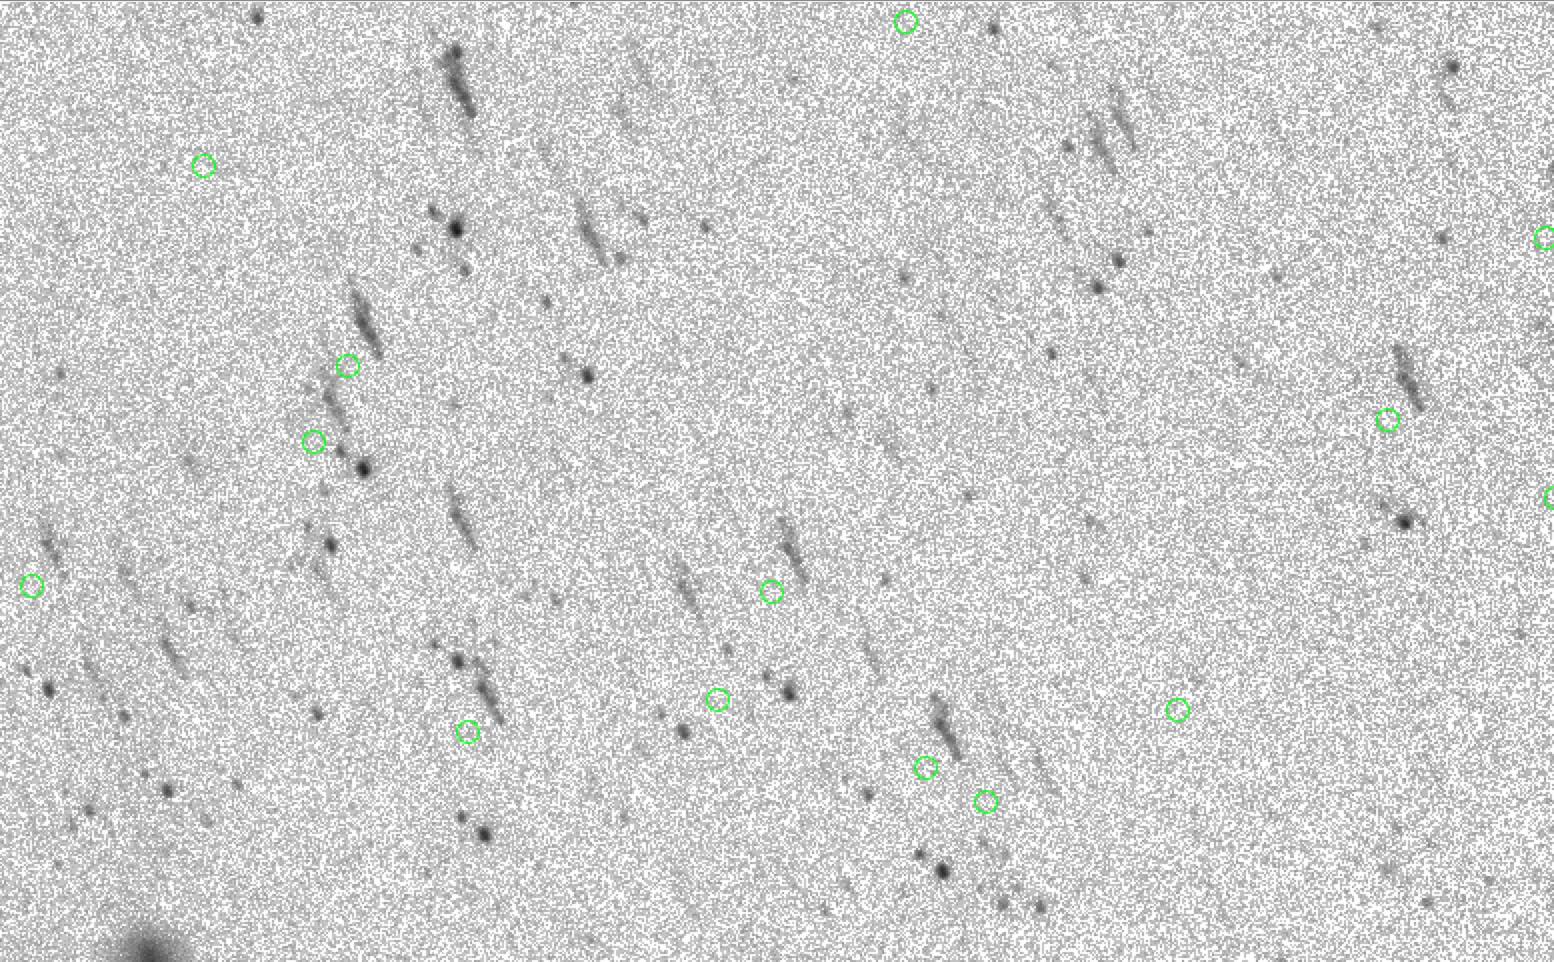
\includegraphics[width=0.49\textwidth]{figures/pip1}
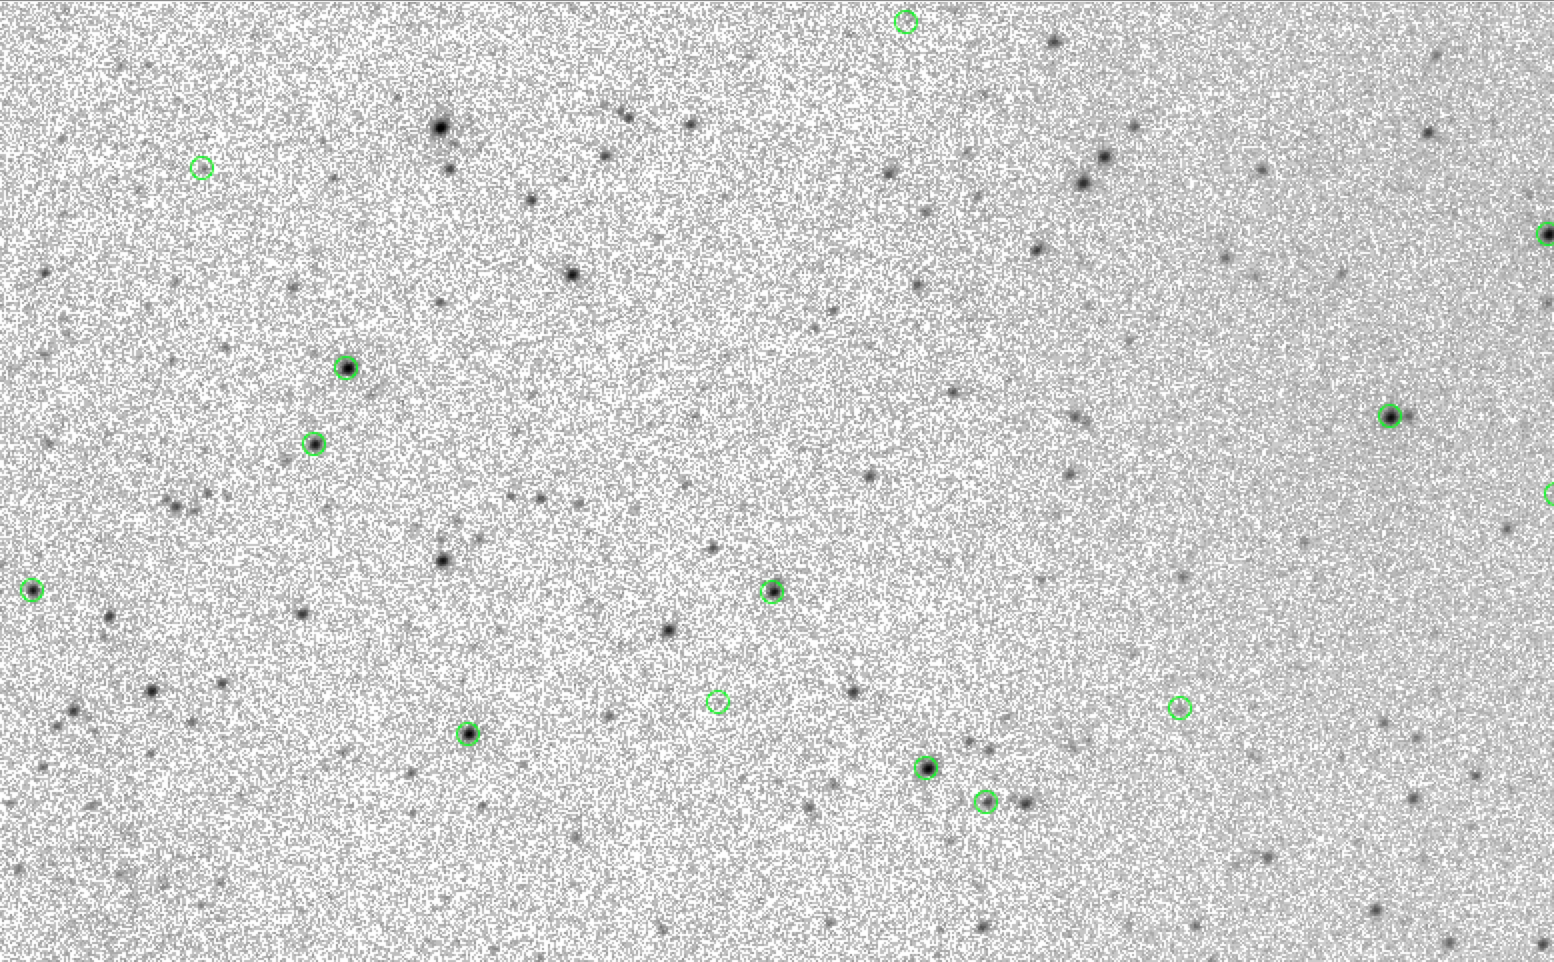
\includegraphics[width=0.49\textwidth]{figures/cal1}
\end{center}
\caption{
  \label{map2}
  Side-by-side comparison with the images generated by the original calibration from the telescope.
  \emph{Left:} images from the orignal pipeline;
  \emph{Right}: images from our pipeline.
  The stars from Tycho 2 catalog are marked by the green circle.
}
\end{figure}

\begin{figure}[p]
\begin{center}
\includegraphics[width=1.\textwidth]{figures/overlap}
\end{center}
\caption{
  \label{map3}
  All sky Mollweide projection in Galactic coordinates of the NUV intensity maps.
  The \asc\ data are plot in grey scale.
  The \msc\ data are plot in RdBu scale.
  The \scanmode\ data are in Viridis scale. 
}
\end{figure}

\begin{figure}[p]
\begin{center}
\includegraphics[width=0.99\textwidth]{figures/multi1}
\end{center}
\caption{
  \label{map4}
  The Galactic Plane in multi-wavelength. From top to bottom, the data are from:
  \project{Planck} 100 $GHz$; \project{Wise} 3.4 $\mu m$; H-alpha; \cause.
}
\end{figure}

\section{Discussion}
\label{ds}
improvements:
\begin{enumerate}
\item apply q and ya correction instead of cutting the photon list
\item measure different sensitivity maps for stars and background.
\end{enumerate}

In this paper the photons with $Q<=5$ or $Y_A<2$ are removed.


\clearpage
\bibliography{gs}
\clearpage

\end{document}
